\documentclass[sigconf,review,anonymous]{acmart}
\acmConference[ISSTA 2022]{ACM SIGSOFT International Symposium on Software Testing and Analysis}{18-22 July, 2022}{Daejeon, South Korea}
%% Conference information
%% Supplied to authors by publisher for camera-ready submission;
%% use defaults for review submission.
%% \acmConference[PL'17]{ACM SIGPLAN Conference on Programming Languages}{January 01--03, 2017}{New York, NY, USA}
%% \acmConference[ESEC/FSE 2020]{The 28th ACM Joint European Software Engineering Conference and Symposium on the Foundations of Software Engineering}{8 - 13 November, 2020}{Sacramento, California, United States}
%% \acmYear{2017}
%% \acmISBN{} % \acmISBN{978-x-xxxx-xxxx-x/YY/MM}
%% \acmDOI{} % \acmDOI{10.1145/nnnnnnn.nnnnnnn}
%% \startPage{1}

%% Copyright information
%% Supplied to authors (based on authors' rights management selection;
%% see authors.acm.org) by publisher for camera-ready submission;
%% use 'none' for review submission.
%% \setcopyright{none}
%\setcopyright{acmcopyright}
%\setcopyright{acmlicensed}
%\setcopyright{rightsretained}
%\copyrightyear{2017}           %% If different from \acmYear

%% Bibliography style
\bibliographystyle{ACM-Reference-Format}
%% Citation style
%\citestyle{acmauthoryear}  %% For author/year citations
\citestyle{acmnumeric}     %% For numeric citations % PLDI: default citation style is numeric
%\setcitestyle{nosort}      %% With 'acmnumeric', to disable automatic
                            %% sorting of references within a single citation;
                            %% e.g., \cite{Smith99,Carpenter05,Baker12}
                            %% rendered as [14,5,2] rather than [2,5,14].
%\setcitesyle{nocompress}   %% With 'acmnumeric', to disable automatic
                            %% compression of sequential references within a
                            %% single citation;
                            %% e.g., \cite{Baker12,Baker14,Baker16}
                            %% rendered as [2,3,4] rather than [2-4].

%% Use macros

%%% macros.tex
%%% Import packages, define utility commands and define macros
%%% Version 1.2.0

%%%----------
%%% Imports

%%% Text Formatting
\usepackage{microtype}
\usepackage{xspace}
\usepackage{xcolor}
\usepackage{graphicx}
\usepackage[normalem]{ulem} % normalem do not replace \emph to underline
\usepackage{amsmath}
\usepackage{enumitem}
\usepackage{adjustbox}

%%% Reference, Citation and Link
\usepackage{hyperref}
%\usepackage{url}
\usepackage{breakurl}
%\usepackage{cite}

%%% Tables
\usepackage{booktabs}
\usepackage{multirow}
\usepackage{makecell}
\usepackage{ragged2e}

%%% Plots
\usepackage{caption}
%\usepackage{subcaption}
%\usepackage{subfloat}
%\usepackage{wrapfig}
\usepackage{subfig}

% Code
\usepackage{algorithm}
\usepackage{algpseudocode} 
\usepackage{listings}

% Tikz Figs
\usepackage{tikz}
%\usepackage{pgf-umlsd} % for flow diagram
\usetikzlibrary{calc}
\usetikzlibrary{shapes.geometric}
\usetikzlibrary{decorations.pathreplacing}
\usetikzlibrary{positioning}
%\usetikzlibrary{shapes}

%%% Miscellaneous
%\usepackage{flushend} % balance the end of double column document
\usepackage{datetime} % for getting current date time

%%% defs-logic.tex
%%% Utility Commands for Logic Symbols
%%% Version 1.1.0

%%% Basic Logic
% True & False
\newcommand{\ltrue}{\top} % ⊤
\newcommand{\lfalse}{\bot} % ⊥

% Operators
% \land ∧
% \lor ∨
% \lnot ¬
\newcommand{\limply}{\rightarrow} % →
\newcommand{\liff}{\leftrightarrow} % ↔
\newcommand{\lcofactor}{\downarrow} % ↓

\newcommand{\llimply}{\Rightarrow} % ⇒
\newcommand{\lliff}{\Leftrightarrow} % ⇔
\newcommand{\lsat}{\vDash} % ⊨
\newcommand{\lnsat}{\nvDash} % ⊭

% Quantifiers
\newcommand{\lqall}[1]{\forall #1.~} % ∀x.
\newcommand{\lqexist}[1]{\exists #1.~} % ∃x.
\newcommand{\lqallOnly}[1]{\forall #1 } % ∀x
\newcommand{\lqexistOnly}[1]{\exists #1 } % ∃x

% Big Operators
\newcommand{\lAnd}[1]{\bigwedge_{\substack{#1}}} % ⋀
\newcommand{\lOr}[1]{\bigvee_{\substack{#1}}} % ⋁

%%% Set
\newcommand{\set}[1]{\{#1\}} % {x, y, z}
\newcommand{\Set}[1]{\left\{#1\right\}} % \left{ x, y, z \right}
\newcommand{\tuple}[1]{\langle#1\rangle} % <a, b, c>
\newcommand{\Tuple}[1]{\left\langle#1\right\rangle} % \left< a, b, c \right>

\newcommand{\sunion}{\cup} % ∪
\newcommand{\sinter}{\cap} % ∩
 % for logic symbols
%%% defs-code.tex
%%% Utility Commands for Code Listings
%%% Version 1.0.2

%%%==========
%%% COPIED FROM vkuncak/doc/vmcai09/defs.tex
\definecolor{gray}{RGB}{211,211,211}
\newcommand{\jbasicstyle}{\small\sffamily} % Style of code
\newcommand{\textcode}[1]{{#1}}
\newcommand{\jnumberstyle}{\scriptsize}
\newcommand{\Hilight}{\makebox[0pt][l]{\color{gray}\rule[-3pt]{0.80\linewidth}{9pt}}}

\colorlet{punct}{red!60!black}
\definecolor{background}{HTML}{EEEEEE}
\definecolor{delim}{RGB}{20,105,176}
\colorlet{numb}{magenta!60!black}

\makeatletter
\newenvironment{btHighlight}[1][]
{\begingroup\tikzset{bt@Highlight@par/.style={#1}}\begin{lrbox}{\@tempboxa}}
{\end{lrbox}\bt@HL@box[bt@Highlight@par]{\@tempboxa}\endgroup}

\newcommand\btHL[1][]{%
  \begin{btHighlight}[#1]\bgroup\aftergroup\bt@HL@endenv%
}
\def\bt@HL@endenv{%
  \end{btHighlight}%
  \egroup
}
\newcommand{\bt@HL@box}[2][]{%
  \tikz[#1]{%
    \pgfpathrectangle{\pgfpoint{1pt}{0pt}}{\pgfpoint{\wd #2}{\ht #2}}%
    \pgfusepath{use as bounding box}%
    \node[anchor=base west, fill=orange!30,outer sep=0pt,inner xsep=1pt, inner ysep=0pt, rounded corners=1pt, minimum height=\ht\strutbox,#1]{\raisebox{1pt}{\strut}\strut\usebox{#2}};
  }%
}

\newenvironment{btHighlightLine}[1][]
{\begingroup\tikzset{bt@HighlightLine@par/.style={#1}}\begin{lrbox}{\@tempboxa}}
{\end{lrbox}\bt@HLLine@box[bt@HighlightLine@par]{\@tempboxa}\endgroup}

\newcommand\btHLLine[1][]{%
  \begin{btHighlightLine}[#1]\bgroup\aftergroup\bt@HLLine@endenv%
}
\def\bt@HLLine@endenv{%
  \end{btHighlightLine}%
  \egroup
}
\newcommand{\bt@HLLine@box}[2][]{%
  \tikz[#1]{%
    \pgfpathrectangle{\pgfpoint{0pt}{-1pt}}{\pgfpoint{\wd #2}{\ht #2}}%
    \pgfusepath{use as bounding box}%
    \node[anchor=base west, fill=orange!30,outer sep=0pt,inner xsep=0pt, inner ysep=0pt, minimum height=\ht\strutbox+3pt, minimum width=4.1cm,#1] (line-bg) {};
    \node[right = 0 of line-bg.west, outer sep=0pt, inner xsep=0pt, inner ysep=0pt]{\raisebox{0pt}{\strut}\strut\usebox{#2}};
  }%
}
\makeatother

% Disable tikz's error message complaining redefining dollor-sign.  WARNING: this may indeed cause problems but hopefully not
\makeatletter
\global\let\tikz@ensure@dollar@catcode=\relax
\makeatother


\lstdefinelanguage{pseudo}
{
  morekeywords={},
  keywordstyle=\bfseries,
  lineskip=-0.1em,
  numbers=left, % none for no numbers
  numberstyle=\jnumberstyle,
  numbersep=4pt,
  basicstyle=\jbasicstyle,
  breaklines=true,
  breakautoindent=true,
  tabsize=2,
  columns=fullflexible,
  morecomment=*[l][\textsl]{//},
  mathescape=true,
  xleftmargin=10pt,
%  mathescape=false,
}

\lstdefinelanguage{todo-comment}
{
  morekeywords={},
  keywordstyle=\bfseries,
  lineskip=-0.1em,
  numbers=none,
  basicstyle=\jbasicstyle,
  breaklines=true,
  breakautoindent=true,
  tabsize=2,
  columns=fullflexible,
  morecomment=*[l][\textsl]{//},
  mathescape=true,
  xleftmargin=-10pt,
%  mathescape=false,
}

\lstdefinelanguage{json-pretty}
{
  basicstyle=\normalfont\ttfamily,
  numbers=none,
  stepnumber=1,
  numbersep=8pt,
  showstringspaces=true,
  breaklines=true,
  %% frame=single,
  %% backgroundcolor=\color{gray},
  literate=
    *{0}{{{\color{numb}0}}}{1}
     {1}{{{\color{numb}1}}}{1}
     {2}{{{\color{numb}2}}}{1}
     {3}{{{\color{numb}3}}}{1}
     {4}{{{\color{numb}4}}}{1}
     {5}{{{\color{numb}5}}}{1}
     {6}{{{\color{numb}6}}}{1}
     {7}{{{\color{numb}7}}}{1}
     {8}{{{\color{numb}8}}}{1}
     {9}{{{\color{numb}9}}}{1}
     {:}{{{\color{punct}{:}}}}{1}
     {,}{{{\color{punct}{,}}}}{1}
     {\{}{{{\color{delim}{\{}}}}{1}
     {\}}{{{\color{delim}{\}}}}}{1}
     {[}{{{\color{delim}{[}}}}{1}
     {]}{{{\color{delim}{]}}}}{1},
}

\lstset{escapeinside={(*@}{@*)}}

\newcommand{\JsonIn}[1]{{\lstinline[language=json-pretty, basicstyle=\small\ttfamily]@#1@}}

%%%==========
 % for code listings

%%%----------
%%% Utility Commands
\newcommand{\XSpace}[1]{}
\newcommand{\XComment}[1]{}
\newcommand{\Fix}[1]{\textcolor{red}{#1}}
%\newcommand{\CR}[2]{\textcolor{blue}{#1}\textcolor{brown}{\sout{#2}}}
\newcommand{\CR}[2]{#1}
\newcommand{\EditAdd}[1]{\textcolor{green}{[#1]}}
\newcommand{\EditRm}[1]{\textcolor{red}{[\sout{#1}]}}
\newcommand{\EditMod}[2]{\textcolor{red}{[\sout{#1}]}\textcolor{green}{[#2]}}
\newcommand{\DefMacro}[2]{\expandafter\newcommand\csname rmk-#1\endcsname{#2}}
\newcommand{\UseMacro}[1]{\csname rmk-#1\endcsname}
\newcommand{\CfgStmtTableCaptionVSpace}{-5pt}
\newcommand{\ResultTableCaptionVSpace}{-5pt}
\newcommand{\ReqTableVSpace}{-5pt}
\newcommand{\SelfBleuTableVSpace}{-5pt}
\newcommand{\RetrainDebugTableVSpace}{-5pt}
\newcommand{\ManualStudyTableVSpace}{-5pt}
\newcommand{\TestResultsTableVSpace}{-5pt}
\newcommand{\romnum}[1]{\uppercase\expandafter{\romannumeral #1\relax}}

\newcommand{\jl}[1]{\textcolor{teal}{JL: #1}}
\newcommand{\sw}[1]{\textcolor{purple}{Shiyi: #1}}
\newcommand{\wy}[1]{\textcolor{blue}{WY: #1}}
\newcommand{\cm}[1]{\textcolor{red}{Simin: #1}}
\newcommand{\TODO}[1]{\textcolor{red}{TODO: #1}}

\newcommand{\MyPara}[1]{\vspace{0pt}\noindent\textbf{#1}.}
\newcommand{\MyParaOnly}[1]{\noindent\textbf{#1}}
\newcommand{\reducedstrut}{\vrule width 0pt height .9\ht\strutbox depth .9\dp\strutbox\relax}
\newcommand{\InputWithSpace}[1]{\bgroup\def\arraystretch{1.2}\input{#1}\egroup}
\newcommand{\Code}[1]{{\ifmmode{\mathtt{#1}}\else$\mathtt{#1}$\fi}}
\newcommand{\CodeIn}[1]{{\ifmmode{\mathtt{#1}}\else$\mathtt{#1}$\fi}}
\newcommand{\ColorBack}[1]{%
  \begingroup
  \setlength{\fboxsep}{0pt}%
  \colorbox{purple!20}{\reducedstrut#1\/}%
  \endgroup
}

% for table headers
\newcommand{\specialcell}[2][c]{%
  \begin{tabular}[#1]{@{}c@{}}#2\end{tabular}}
\newcolumntype{R}[1]{>{\RaggedLeft\arraybackslash}p{#1}}
\newcolumntype{L}[1]{>{\RaggedRight\arraybackslash}p{#1}}
\def\clap#1{\hbox to 0pt{\hss#1\hss}}

%%% TEXT
\newcommand{\Title}{Programming Language Representation with Semantic-level Structure}

\newcommand{\TreeSitterURL}{https://github.com/tree-sitter/tree-sitter}
\newcommand{\Dxp}{DeepXplore}
\newcommand{\Denas}{DENAS}

\newcommand{\tool}{S$^2$LCT\xspace}

% Sorted alphabetically, ignoring case
\newcommand{\Model}{Auto-CHECKLIST\xspace}
\newcommand{\Lc}{Linguistic capability\xspace}
\newcommand{\lc}{linguistic capability\xspace}
\newcommand{\lcs}{linguistic capabilities\xspace}
\newcommand{\Cfg}{Context-free grammar\xspace}
\newcommand{\cfg}{context-free grammar\xspace}
\newcommand{\Pcfg}{Probabilistic context-free grammar\xspace}
\newcommand{\pcfg}{probabilistic context-free grammar\xspace}
\newcommand{\lm}{langugae model\xspace}
\newcommand{\lms}{langugae models\xspace}
\newcommand{\Lm}{Langugae Model\xspace}
\newcommand{\dl}{deep learning\xspace}
\newcommand{\Dl}{Deep Learning\xspace}
\newcommand{\ml}{machine learning\xspace}
\newcommand{\ML}{Machine Learning\xspace}
\newcommand{\nl}{natural language\xspace}
\newcommand{\Nl}{Natural language\xspace}
\newcommand{\nlp}{natural language processing\xspace}
\newcommand{\Nlp}{Natural language processing\xspace}
\newcommand{\Sa}{Sentiment analysis\xspace}
\newcommand{\sa}{sentiment analysis\xspace}
\newcommand{\se}{software engineering\xspace}
\newcommand{\Se}{Software Engineering\xspace}
\newcommand{\sota}{state-of-the-art\xspace}
%\newcommand{\Sw}{Software\xspace}
%\newcommand{\sw}{software\xspace}
\newcommand{\pos}{part-of-speech\xspace}
\newcommand{\ho}{hold-out\xspace}
\newcommand{\ie}{i.e.\xspace}
\newcommand{\eg}{e.g.\xspace}
\newcommand{\etal}{et al.\xspace}

\newcommand{\Req}{Requirement\xspace}
\newcommand{\req}{requirement\xspace}
\newcommand{\Prodr}{Production rule\xspace}
\newcommand{\prodr}{production rule\xspace}
\newcommand{\prodrs}{production rules\xspace}
\newcommand{\lhs}{left-hand side\xspace}
\newcommand{\rhs}{right-hand side\xspace}
\newcommand{\mask}{\{MASK\}}
\newcommand{\SareqExOne}{``Short sentences with neutral adjectives and nouns''\xspace}
\newcommand{\SareqExTwo}{``Negated positive with neutral content in the middle''\xspace}
\newcommand{\SareqExThree}{``Short sentences with sentiment-laden adjectives''\xspace}
\newcommand{\Sent}{Sentence\xspace}
\newcommand{\sent}{sentence\xspace}
\newcommand{\sents}{sentences\xspace}
\newcommand{\reqs}{requirements\xspace}
\newcommand{\Pstv}{Positive\xspace}
\newcommand{\pstv}{positive\xspace}
\newcommand{\Neu}{Neutral\xspace}
\newcommand{\neu}{neutral\xspace}
\newcommand{\Ngtv}{Negative\xspace}
\newcommand{\ngtv}{negative\xspace}
\newcommand{\Noun}{Noun\xspace}
\newcommand{\noun}{noun\xspace}
\newcommand{\nns}{nouns\xspace}
\newcommand{\Vb}{Verb\xspace}
\newcommand{\vb}{verb\xspace}
\newcommand{\vbs}{verbs\xspace}
\newcommand{\Adj}{Adjective\xspace}
\newcommand{\adj}{adjective\xspace}
\newcommand{\adjs}{adjectives\xspace}
\newcommand{\selfbleu}{Self-BLEU\xspace}

\newcommand{\Nn}{neural network\xspace}
\newcommand{\nn}{neural network\xspace}
\newcommand{\Bert}{BERT-base\xspace}
\newcommand{\BertAcc}{92.43\%\xspace}
\newcommand{\Roberta}{RoBERTa-base\xspace}
\newcommand{\RobertaAcc}{94.04\%\xspace}
\newcommand{\Dbert}{DistilBERT-base\xspace}
\newcommand{\DbertAcc}{91.3\%\xspace}

\newcommand{\Cklst}{CHECKLIST\xspace}
\newcommand{\Trb}{Treebank\xspace}
\newcommand{\trb}{treebank\xspace}
\newcommand{\Wsj}{Wall Street Journal\xspace}
\newcommand{\Nltk}{NLTK\xspace}
\newcommand{\Spacy}{Spacy\xspace}
\newcommand{\Wrdnt}{WordNet\xspace}
\newcommand{\Swn}{SentiWordNet\xspace}
\newcommand{\Sstt}{Stanford Sentiment Treebank version 1\xspace}
\newcommand{\spacy}{SpaCy\xspace}
\newcommand{\bertsamodel}{textattack/bert-base-uncased-SST-2\xspace}
\newcommand{\robertasamodel}{textattack/roberta-base-SST-2\xspace}
\newcommand{\disbertsamodel}{distilbert-base-uncased-finetuned-sst-2-english\xspace}

%% Table
\newcommand{\tStatement}{\textbf{Statement Types}}
\newcommand{\tModel}{\textbf{Models}}
\newcommand{\tMetric}{\textbf{Metrics}}
\newcommand{\tLc}{\textbf{Linguistic capability}}
\newcommand{\tRules}{\textbf{Search rule and transformation template}}
\newcommand{\tOurNumData}{\textbf{\sharp~Data (\tool)}}
\newcommand{\tChecklistNumData}{\textbf{\sharp~Data (\Cklst)}}
\newcommand{\tOurSelfBleuScore}{\textbf{\selfbleu score (\tool)}}
\newcommand{\tChecklistSelfBleuScore}{\textbf{\selfbleu score (\Cklst)}}
\newcommand{\tApproach}{\textbf{Approach}}
\newcommand{\tRetrainlc}{\textbf{RetrainLC}}
\newcommand{\tEvallc}{\textbf{EvalLC}}
\newcommand{\tNumfailpass}{\textbf{\#Fail2Pass}}
\newcommand{\tNumfailbeforeretrain}{\textbf{\#Fail(BeforeRetrain)}}
\newcommand{\tNumpassbeforeretrain}{\textbf{\#Pass(BeforeRetrain)}}
\newcommand{\tNumfailafterretrain}{\textbf{\#Fail(AfterRetrain)}}
\newcommand{\tNumpassafterretrain}{\textbf{\#Pass(AfterRetrain)}}
\newcommand{\tSentType}{\textbf{Type}}
\newcommand{\tNumTestCases}{\textbf{\#Testcases}}
\newcommand{\tAvgLabelCons}{\textbf{LabelConsistency}}
\newcommand{\tAvgLCRel}{\textbf{LcRelevancy}}

\newcommand{\tNumBlSents}{\textbf{Cklst \#TCs}}
\newcommand{\tNumBlFail}{\textbf{Cklst \#Fails}}
\newcommand{\tNumSeeds}{\textbf{\tool\#Seeds}}
\newcommand{\tNumSeedFail}{\textbf{\tool Seed \#Fails}}
\newcommand{\tNumExps}{\textbf{\tool\#Exps}}
\newcommand{\tNumExpFail}{\textbf{\tool Exp \#Fails}}
\newcommand{\tNumPasstoFail}{\textbf{\tool\#PassToFail}}


%% Fig Caption
\newcommand{\OverviewFigCaption}{Overview of \tool.\label{fig:overview}}
\newcommand{\SearchRequirementExampleFigCaption}{Search requirement
on the linguistic capability of \SareqExOne.\label{fig:SearchReqEx}}
\newcommand{\TransformRequirementExampleSubFigCaption}{Transform requirement\label{fig:TransformReqSubEx}}
\newcommand{\TransformTemplateExampleSubFigCaption}{Transform template\label{fig:TransformTempSubEx}}
\newcommand{\TransformRequirementExampleFigCaption}{Transform
requirement (\ref{fig:TransformReqSubEx}) and its template
(\ref{fig:TransformTempSubEx}) on the linguistic capability of \SareqExTwo.\label{fig:TransformReqEx}}
\newcommand{\ProdDiffAlgCaption}{Pseudocode of Production differentiation\label{code:ProdDiffAlg}}
\newcommand{\RunningExCaption}{Example of masked sentence generation. \sw{Expansion: Or both \mask. -> Masked sentence: Or both {MASK.}}\label{fig:ExpEx}}
\newcommand{\CklstTemplateFigCaption}{Example of \Cklst templates on \lc of \SareqExThree.\label{code:TempEx}}

%% Table Caption
\newcommand{\ReqTableCaption}{Search rules and transformation templates for linguistic capabilities. \sw{Add transformation templates. May need to find a better specification language.}.\label{tab:specification}\vspace{\ReqTableVSpace}}
\newcommand{\ResultTableCaption}{Results on \Nlp tasks
of \Ccd, \Ctr, \Cref repectively.\label{table:Result}\vspace{-5pt}}
\newcommand{\SelfBleuTableCaption}{\selfbleu scores over testcases
from \tool and \Cklst}
\newcommand{\RetrainDebugTableCaption}{Result of retraining on
each \lc and the evaluation of the retrained model.\label{table:RetrainDebug}}
\newcommand{\ManualStudyTableCaption}{Aggregated Statistics of manual
study of label consistency and \lc relevancy of \tool generated
testcases compared with human annotations.\label{table:ManualStudy}}
\newcommand{\TestResultsTableCaption}{Comparison of evaluation of \Bert, \Roberta and
\Dbert \sa models on \tool and \Cklst (Cklst) testcases (TCs). Due to the spatial constraints
of table, \Bert, \Roberta and
\Dbert models are denoted as BERT, RoBERTa and dstBERT respectively.\label{table:TestResult}}


%%% NUMBRERS

%% Automatically generated by pyutil.latex 

\DefMacro{lc_1_desc}{Short sentences with neutral adjectives and nouns}
\DefMacro{lc_1_search}{\textbf{Search}~seed=\{length: <10; include: neutral adjs \& neutral nouns;~exlcude: pos adjs \& neg adjs \& pos nouns \& neg nouns; label: neutral\}}
\DefMacro{lc_1_transform}{\textbf{Transform}~N/A}
\DefMacro{lc_2_desc}{Short sentences with sentiment-laden adjectives}
\DefMacro{lc_2_search}{\textbf{Search}~seed=\{length: <10; include: pos adjs;~exlcude: neg adjs \& neg verbs \& neg nouns; label: pos\} | \{length: <10; include: neg adjs;exclude: pos adjs \& pos verbs \& pos nouns \& neg verbs \& neg nouns; label: neg\}}
\DefMacro{lc_2_transform}{\textbf{Transform}~N/A}
\DefMacro{lc_3_desc}{Sentiment change over time, present should prevail}
\DefMacro{lc_3_search}{\textbf{Search}~pos\_sent=\{label: pos\}, neg\_sent=\{label: neg\}}
\DefMacro{lc_3_transform}{\textbf{Transform}~seed=\{['Previously, I used to like it saying that','Last time, I agreed with saying that','I liked it much as to say that']+[neg\_sent, pos\_sent]+['but', 'although', 'on the other hand']+['now I don't like it.', 'now I hate it.']\} | \{['I used to disagree with saying that','Last time, I didn't like it saying that','I hated it much as to say that']+[neg\_sent, pos\_sent]+['but', 'although', 'on the other hand']+['now I like it.']\}}
\DefMacro{lc_4_desc}{Negated negative should be positive or neutral}
\DefMacro{lc_4_search}{\textbf{Search}~demonstrative\_sent=\{start: [This, That, These, Those] + [is, are]; label: neg\}}
\DefMacro{lc_4_transform}{\textbf{Transform}~seed=negation of demonstrative\_sent (['is'] -> ['is not', 'isn't'], ['are'] -> ['are not', 'aren't'])}
\DefMacro{lc_5_desc}{Negated neutral should still be neutral}
\DefMacro{lc_5_search}{\textbf{Search}~demonstrative\_sent=\{start: [This, That, These, Those] + [is, are]; label: neutral\}}
\DefMacro{lc_5_transform}{\textbf{Transform}~negation of demonstrative\_sent}
\DefMacro{lc_6_desc}{Negation of negative at the end, should be positive or neutral}
\DefMacro{lc_6_search}{\textbf{Search}~neg\_sent=\{label: neg\}}
\DefMacro{lc_6_transform}{\textbf{Transform}~seed=\{['I agreed that', 'I thought that']+[neg\_sent]+['but it wasn't', 'but I didn't']\}}
\DefMacro{lc_7_desc}{Negated positive with neutral content in the middle}
\DefMacro{lc_7_search}{\textbf{Search}~pos\_sent=\{length: <20; label: pos\}, neutral\_sent=\{length: <20; label: neutral\}}
\DefMacro{lc_7_transform}{\textbf{Transform}~seed=\{['I wouldn't say,', 'I do not think,', 'I don't agree with,']+[neutral\_sent]+[pos\_sent]\}}
\DefMacro{lc_8_desc}{Author sentiment is more important than others}
\DefMacro{lc_8_search}{\textbf{Search}~pos\_sent=\{label:pos\}, neg\_sent=\{label: neg\}}
\DefMacro{lc_8_transform}{\textbf{Transform}~seed=\{[temp1]+[pos\_sent]+[temp2]+[neg\_sent]\} | \{[temp1]+[neg\_sent]+[temp2]+[pos\_sent]\} where temp1=\{['Some people think that', 'Many people agree with that', 'They think that', 'You agree with that'], temp2=['but I think that']\}}
\DefMacro{lc_9_desc}{Parsing sentiment in (question, yes) form}
\DefMacro{lc_9_search}{\textbf{Search}~pos\_sent=\{label: pos\}, neg\_sent=\{label: neg\}}
\DefMacro{lc_9_transform}{\textbf{Transform}~seed=\{['Do I think that', 'Do I agree that']+[pos\_sent | neg\_sent]+['? yes']\}}
\DefMacro{lc_10_desc}{Parsing positive sentiment in (question, no) form}
\DefMacro{lc_10_search}{\textbf{Search}~pos\_sent=\{label: pos\}}
\DefMacro{lc_10_transform}{\textbf{Transform}~seed=\{['Do I think that', 'Do I agree that']+[pos\_sent]+['? no']\}}
\DefMacro{lc_11_desc}{Parsing negative sentiment in (question, no) form}
\DefMacro{lc_11_search}{\textbf{Search}~neg\_sent=\{label: neg\}}
\DefMacro{lc_11_transform}{\textbf{Transform}~seed=\{['Do I think that', 'Do I agree that']+[neg\_sent]+['? no']\}}

%% \input{tables/selfbleu-numbers}
%% 
%% Automatically generated by pyutil.latex 

\DefMacro{retrain_debug_approach_0}{Retrain:Ours::Test:Checklist}
\DefMacro{retrain_debug_retrained_lc_0}{parsing sentiment in (question  yes) form}
\DefMacro{retrain_debug_eval_lc_0}{Negated positive with neutral content in the middle}
\DefMacro{retrain_debug_num_fail2pass_0}{0}
\DefMacro{retrain_debug_num_fail_orig_0}{860}
\DefMacro{retrain_debug_num_pass_orig_0}{140}
\DefMacro{retrain_debug_num_fail_retrained_0}{1000}
\DefMacro{retrain_debug_num_pass_retrained_0}{0}
\DefMacro{retrain_debug_approach_1}{Retrain:Ours::Test:Checklist}
\DefMacro{retrain_debug_retrained_lc_1}{parsing sentiment in (question  yes) form}
\DefMacro{retrain_debug_eval_lc_1}{Short sentences with sentiment-laden adjectives}
\DefMacro{retrain_debug_num_fail2pass_1}{0}
\DefMacro{retrain_debug_num_fail_orig_1}{26}
\DefMacro{retrain_debug_num_pass_orig_1}{8632}
\DefMacro{retrain_debug_num_fail_retrained_1}{8658}
\DefMacro{retrain_debug_num_pass_retrained_1}{0}
\DefMacro{retrain_debug_approach_2}{Retrain:Ours::Test:Checklist}
\DefMacro{retrain_debug_retrained_lc_2}{parsing sentiment in (question  yes) form}
\DefMacro{retrain_debug_eval_lc_2}{parsing sentiment in (question, yes) form}
\DefMacro{retrain_debug_num_fail2pass_2}{1082}
\DefMacro{retrain_debug_num_fail_orig_2}{1793}
\DefMacro{retrain_debug_num_pass_orig_2}{7411}
\DefMacro{retrain_debug_num_fail_retrained_2}{1203}
\DefMacro{retrain_debug_num_pass_retrained_2}{8001}
\DefMacro{retrain_debug_approach_3}{Retrain:Ours::Test:Checklist}
\DefMacro{retrain_debug_retrained_lc_3}{parsing sentiment in (question  yes) form}
\DefMacro{retrain_debug_eval_lc_3}{Author sentiment is more important than of others}
\DefMacro{retrain_debug_num_fail2pass_3}{0}
\DefMacro{retrain_debug_num_fail_orig_3}{3741}
\DefMacro{retrain_debug_num_pass_orig_3}{4787}
\DefMacro{retrain_debug_num_fail_retrained_3}{8528}
\DefMacro{retrain_debug_num_pass_retrained_3}{0}
\DefMacro{retrain_debug_approach_4}{Retrain:Ours::Test:Checklist}
\DefMacro{retrain_debug_retrained_lc_4}{parsing sentiment in (question  yes) form}
\DefMacro{retrain_debug_eval_lc_4}{Short sentences with neutral adjectives and nouns}
\DefMacro{retrain_debug_num_fail2pass_4}{1330}
\DefMacro{retrain_debug_num_fail_orig_4}{1330}
\DefMacro{retrain_debug_num_pass_orig_4}{386}
\DefMacro{retrain_debug_num_fail_retrained_4}{0}
\DefMacro{retrain_debug_num_pass_retrained_4}{1716}
\DefMacro{retrain_debug_approach_5}{Retrain:Ours::Test:Checklist}
\DefMacro{retrain_debug_retrained_lc_5}{parsing sentiment in (question  yes) form}
\DefMacro{retrain_debug_eval_lc_5}{Negated neutral should still be neutral}
\DefMacro{retrain_debug_num_fail2pass_5}{2427}
\DefMacro{retrain_debug_num_fail_orig_5}{2427}
\DefMacro{retrain_debug_num_pass_orig_5}{69}
\DefMacro{retrain_debug_num_fail_retrained_5}{0}
\DefMacro{retrain_debug_num_pass_retrained_5}{2496}
\DefMacro{retrain_debug_approach_6}{Retrain:Ours::Test:Checklist}
\DefMacro{retrain_debug_retrained_lc_6}{parsing sentiment in (question  yes) form}
\DefMacro{retrain_debug_eval_lc_6}{Sentiment change over time, present should prevail}
\DefMacro{retrain_debug_num_fail2pass_6}{0}
\DefMacro{retrain_debug_num_fail_orig_6}{1680}
\DefMacro{retrain_debug_num_pass_orig_6}{6320}
\DefMacro{retrain_debug_num_fail_retrained_6}{8000}
\DefMacro{retrain_debug_num_pass_retrained_6}{0}
\DefMacro{retrain_debug_approach_7}{Retrain:Ours::Test:Checklist}
\DefMacro{retrain_debug_retrained_lc_7}{Short sentences with sentiment-laden adjectives}
\DefMacro{retrain_debug_eval_lc_7}{Negated positive with neutral content in the middle}
\DefMacro{retrain_debug_num_fail2pass_7}{0}
\DefMacro{retrain_debug_num_fail_orig_7}{860}
\DefMacro{retrain_debug_num_pass_orig_7}{140}
\DefMacro{retrain_debug_num_fail_retrained_7}{1000}
\DefMacro{retrain_debug_num_pass_retrained_7}{0}
\DefMacro{retrain_debug_approach_8}{Retrain:Ours::Test:Checklist}
\DefMacro{retrain_debug_retrained_lc_8}{Short sentences with sentiment-laden adjectives}
\DefMacro{retrain_debug_eval_lc_8}{Short sentences with sentiment-laden adjectives}
\DefMacro{retrain_debug_num_fail2pass_8}{0}
\DefMacro{retrain_debug_num_fail_orig_8}{26}
\DefMacro{retrain_debug_num_pass_orig_8}{8632}
\DefMacro{retrain_debug_num_fail_retrained_8}{8658}
\DefMacro{retrain_debug_num_pass_retrained_8}{0}
\DefMacro{retrain_debug_approach_9}{Retrain:Ours::Test:Checklist}
\DefMacro{retrain_debug_retrained_lc_9}{Short sentences with sentiment-laden adjectives}
\DefMacro{retrain_debug_eval_lc_9}{parsing sentiment in (question, yes) form}
\DefMacro{retrain_debug_num_fail2pass_9}{1540}
\DefMacro{retrain_debug_num_fail_orig_9}{1793}
\DefMacro{retrain_debug_num_pass_orig_9}{7411}
\DefMacro{retrain_debug_num_fail_retrained_9}{7644}
\DefMacro{retrain_debug_num_pass_retrained_9}{1560}
\DefMacro{retrain_debug_approach_10}{Retrain:Ours::Test:Checklist}
\DefMacro{retrain_debug_retrained_lc_10}{Short sentences with sentiment-laden adjectives}
\DefMacro{retrain_debug_eval_lc_10}{Author sentiment is more important than of others}
\DefMacro{retrain_debug_num_fail2pass_10}{0}
\DefMacro{retrain_debug_num_fail_orig_10}{3741}
\DefMacro{retrain_debug_num_pass_orig_10}{4787}
\DefMacro{retrain_debug_num_fail_retrained_10}{8528}
\DefMacro{retrain_debug_num_pass_retrained_10}{0}
\DefMacro{retrain_debug_approach_11}{Retrain:Ours::Test:Checklist}
\DefMacro{retrain_debug_retrained_lc_11}{Short sentences with sentiment-laden adjectives}
\DefMacro{retrain_debug_eval_lc_11}{Short sentences with neutral adjectives and nouns}
\DefMacro{retrain_debug_num_fail2pass_11}{1330}
\DefMacro{retrain_debug_num_fail_orig_11}{1330}
\DefMacro{retrain_debug_num_pass_orig_11}{386}
\DefMacro{retrain_debug_num_fail_retrained_11}{0}
\DefMacro{retrain_debug_num_pass_retrained_11}{1716}
\DefMacro{retrain_debug_approach_12}{Retrain:Ours::Test:Checklist}
\DefMacro{retrain_debug_retrained_lc_12}{Short sentences with sentiment-laden adjectives}
\DefMacro{retrain_debug_eval_lc_12}{Negated neutral should still be neutral}
\DefMacro{retrain_debug_num_fail2pass_12}{2427}
\DefMacro{retrain_debug_num_fail_orig_12}{2427}
\DefMacro{retrain_debug_num_pass_orig_12}{69}
\DefMacro{retrain_debug_num_fail_retrained_12}{0}
\DefMacro{retrain_debug_num_pass_retrained_12}{2496}
\DefMacro{retrain_debug_approach_13}{Retrain:Ours::Test:Checklist}
\DefMacro{retrain_debug_retrained_lc_13}{Short sentences with sentiment-laden adjectives}
\DefMacro{retrain_debug_eval_lc_13}{Sentiment change over time, present should prevail}
\DefMacro{retrain_debug_num_fail2pass_13}{0}
\DefMacro{retrain_debug_num_fail_orig_13}{1680}
\DefMacro{retrain_debug_num_pass_orig_13}{6320}
\DefMacro{retrain_debug_num_fail_retrained_13}{8000}
\DefMacro{retrain_debug_num_pass_retrained_13}{0}
\DefMacro{retrain_debug_approach_14}{Retrain:Ours::Test:Checklist}
\DefMacro{retrain_debug_retrained_lc_14}{Short sentences with neutral adjectives and nouns}
\DefMacro{retrain_debug_eval_lc_14}{Negated positive with neutral content in the middle}
\DefMacro{retrain_debug_num_fail2pass_14}{0}
\DefMacro{retrain_debug_num_fail_orig_14}{860}
\DefMacro{retrain_debug_num_pass_orig_14}{140}
\DefMacro{retrain_debug_num_fail_retrained_14}{1000}
\DefMacro{retrain_debug_num_pass_retrained_14}{0}
\DefMacro{retrain_debug_approach_15}{Retrain:Ours::Test:Checklist}
\DefMacro{retrain_debug_retrained_lc_15}{Short sentences with neutral adjectives and nouns}
\DefMacro{retrain_debug_eval_lc_15}{Short sentences with sentiment-laden adjectives}
\DefMacro{retrain_debug_num_fail2pass_15}{0}
\DefMacro{retrain_debug_num_fail_orig_15}{26}
\DefMacro{retrain_debug_num_pass_orig_15}{8632}
\DefMacro{retrain_debug_num_fail_retrained_15}{8658}
\DefMacro{retrain_debug_num_pass_retrained_15}{0}
\DefMacro{retrain_debug_approach_16}{Retrain:Ours::Test:Checklist}
\DefMacro{retrain_debug_retrained_lc_16}{Short sentences with neutral adjectives and nouns}
\DefMacro{retrain_debug_eval_lc_16}{parsing sentiment in (question, yes) form}
\DefMacro{retrain_debug_num_fail2pass_16}{1540}
\DefMacro{retrain_debug_num_fail_orig_16}{1793}
\DefMacro{retrain_debug_num_pass_orig_16}{7411}
\DefMacro{retrain_debug_num_fail_retrained_16}{7644}
\DefMacro{retrain_debug_num_pass_retrained_16}{1560}
\DefMacro{retrain_debug_approach_17}{Retrain:Ours::Test:Checklist}
\DefMacro{retrain_debug_retrained_lc_17}{Short sentences with neutral adjectives and nouns}
\DefMacro{retrain_debug_eval_lc_17}{Author sentiment is more important than of others}
\DefMacro{retrain_debug_num_fail2pass_17}{0}
\DefMacro{retrain_debug_num_fail_orig_17}{3741}
\DefMacro{retrain_debug_num_pass_orig_17}{4787}
\DefMacro{retrain_debug_num_fail_retrained_17}{8528}
\DefMacro{retrain_debug_num_pass_retrained_17}{0}
\DefMacro{retrain_debug_approach_18}{Retrain:Ours::Test:Checklist}
\DefMacro{retrain_debug_retrained_lc_18}{Short sentences with neutral adjectives and nouns}
\DefMacro{retrain_debug_eval_lc_18}{Short sentences with neutral adjectives and nouns}
\DefMacro{retrain_debug_num_fail2pass_18}{1330}
\DefMacro{retrain_debug_num_fail_orig_18}{1330}
\DefMacro{retrain_debug_num_pass_orig_18}{386}
\DefMacro{retrain_debug_num_fail_retrained_18}{0}
\DefMacro{retrain_debug_num_pass_retrained_18}{1716}
\DefMacro{retrain_debug_approach_19}{Retrain:Ours::Test:Checklist}
\DefMacro{retrain_debug_retrained_lc_19}{Short sentences with neutral adjectives and nouns}
\DefMacro{retrain_debug_eval_lc_19}{Negated neutral should still be neutral}
\DefMacro{retrain_debug_num_fail2pass_19}{2427}
\DefMacro{retrain_debug_num_fail_orig_19}{2427}
\DefMacro{retrain_debug_num_pass_orig_19}{69}
\DefMacro{retrain_debug_num_fail_retrained_19}{0}
\DefMacro{retrain_debug_num_pass_retrained_19}{2496}
\DefMacro{retrain_debug_approach_20}{Retrain:Ours::Test:Checklist}
\DefMacro{retrain_debug_retrained_lc_20}{Short sentences with neutral adjectives and nouns}
\DefMacro{retrain_debug_eval_lc_20}{Sentiment change over time, present should prevail}
\DefMacro{retrain_debug_num_fail2pass_20}{0}
\DefMacro{retrain_debug_num_fail_orig_20}{1680}
\DefMacro{retrain_debug_num_pass_orig_20}{6320}
\DefMacro{retrain_debug_num_fail_retrained_20}{8000}
\DefMacro{retrain_debug_num_pass_retrained_20}{0}
\DefMacro{retrain_debug_approach_21}{Retrain:Ours::Test:Checklist}
\DefMacro{retrain_debug_retrained_lc_21}{Sentiment change over time  present should prevail}
\DefMacro{retrain_debug_eval_lc_21}{Negated positive with neutral content in the middle}
\DefMacro{retrain_debug_num_fail2pass_21}{0}
\DefMacro{retrain_debug_num_fail_orig_21}{860}
\DefMacro{retrain_debug_num_pass_orig_21}{140}
\DefMacro{retrain_debug_num_fail_retrained_21}{1000}
\DefMacro{retrain_debug_num_pass_retrained_21}{0}
\DefMacro{retrain_debug_approach_22}{Retrain:Ours::Test:Checklist}
\DefMacro{retrain_debug_retrained_lc_22}{Sentiment change over time  present should prevail}
\DefMacro{retrain_debug_eval_lc_22}{Short sentences with sentiment-laden adjectives}
\DefMacro{retrain_debug_num_fail2pass_22}{0}
\DefMacro{retrain_debug_num_fail_orig_22}{26}
\DefMacro{retrain_debug_num_pass_orig_22}{8632}
\DefMacro{retrain_debug_num_fail_retrained_22}{8658}
\DefMacro{retrain_debug_num_pass_retrained_22}{0}
\DefMacro{retrain_debug_approach_23}{Retrain:Ours::Test:Checklist}
\DefMacro{retrain_debug_retrained_lc_23}{Sentiment change over time  present should prevail}
\DefMacro{retrain_debug_eval_lc_23}{parsing sentiment in (question, yes) form}
\DefMacro{retrain_debug_num_fail2pass_23}{1540}
\DefMacro{retrain_debug_num_fail_orig_23}{1793}
\DefMacro{retrain_debug_num_pass_orig_23}{7411}
\DefMacro{retrain_debug_num_fail_retrained_23}{7644}
\DefMacro{retrain_debug_num_pass_retrained_23}{1560}
\DefMacro{retrain_debug_approach_24}{Retrain:Ours::Test:Checklist}
\DefMacro{retrain_debug_retrained_lc_24}{Sentiment change over time  present should prevail}
\DefMacro{retrain_debug_eval_lc_24}{Author sentiment is more important than of others}
\DefMacro{retrain_debug_num_fail2pass_24}{0}
\DefMacro{retrain_debug_num_fail_orig_24}{3741}
\DefMacro{retrain_debug_num_pass_orig_24}{4787}
\DefMacro{retrain_debug_num_fail_retrained_24}{8528}
\DefMacro{retrain_debug_num_pass_retrained_24}{0}
\DefMacro{retrain_debug_approach_25}{Retrain:Ours::Test:Checklist}
\DefMacro{retrain_debug_retrained_lc_25}{Sentiment change over time  present should prevail}
\DefMacro{retrain_debug_eval_lc_25}{Short sentences with neutral adjectives and nouns}
\DefMacro{retrain_debug_num_fail2pass_25}{1330}
\DefMacro{retrain_debug_num_fail_orig_25}{1330}
\DefMacro{retrain_debug_num_pass_orig_25}{386}
\DefMacro{retrain_debug_num_fail_retrained_25}{0}
\DefMacro{retrain_debug_num_pass_retrained_25}{1716}
\DefMacro{retrain_debug_approach_26}{Retrain:Ours::Test:Checklist}
\DefMacro{retrain_debug_retrained_lc_26}{Sentiment change over time  present should prevail}
\DefMacro{retrain_debug_eval_lc_26}{Negated neutral should still be neutral}
\DefMacro{retrain_debug_num_fail2pass_26}{2427}
\DefMacro{retrain_debug_num_fail_orig_26}{2427}
\DefMacro{retrain_debug_num_pass_orig_26}{69}
\DefMacro{retrain_debug_num_fail_retrained_26}{0}
\DefMacro{retrain_debug_num_pass_retrained_26}{2496}
\DefMacro{retrain_debug_approach_27}{Retrain:Ours::Test:Checklist}
\DefMacro{retrain_debug_retrained_lc_27}{Sentiment change over time  present should prevail}
\DefMacro{retrain_debug_eval_lc_27}{Sentiment change over time, present should prevail}
\DefMacro{retrain_debug_num_fail2pass_27}{0}
\DefMacro{retrain_debug_num_fail_orig_27}{1680}
\DefMacro{retrain_debug_num_pass_orig_27}{6320}
\DefMacro{retrain_debug_num_fail_retrained_27}{7888}
\DefMacro{retrain_debug_num_pass_retrained_27}{112}
\DefMacro{retrain_debug_approach_28}{Retrain:Ours::Test:Checklist}
\DefMacro{retrain_debug_retrained_lc_28}{Negated positive with neutral content in the middle}
\DefMacro{retrain_debug_eval_lc_28}{Negated positive with neutral content in the middle}
\DefMacro{retrain_debug_num_fail2pass_28}{840}
\DefMacro{retrain_debug_num_fail_orig_28}{860}
\DefMacro{retrain_debug_num_pass_orig_28}{140}
\DefMacro{retrain_debug_num_fail_retrained_28}{20}
\DefMacro{retrain_debug_num_pass_retrained_28}{980}
\DefMacro{retrain_debug_approach_29}{Retrain:Ours::Test:Checklist}
\DefMacro{retrain_debug_retrained_lc_29}{Negated positive with neutral content in the middle}
\DefMacro{retrain_debug_eval_lc_29}{Short sentences with sentiment-laden adjectives}
\DefMacro{retrain_debug_num_fail2pass_29}{0}
\DefMacro{retrain_debug_num_fail_orig_29}{26}
\DefMacro{retrain_debug_num_pass_orig_29}{8632}
\DefMacro{retrain_debug_num_fail_retrained_29}{8658}
\DefMacro{retrain_debug_num_pass_retrained_29}{0}
\DefMacro{retrain_debug_approach_30}{Retrain:Ours::Test:Checklist}
\DefMacro{retrain_debug_retrained_lc_30}{Negated positive with neutral content in the middle}
\DefMacro{retrain_debug_eval_lc_30}{parsing sentiment in (question, yes) form}
\DefMacro{retrain_debug_num_fail2pass_30}{1540}
\DefMacro{retrain_debug_num_fail_orig_30}{1793}
\DefMacro{retrain_debug_num_pass_orig_30}{7411}
\DefMacro{retrain_debug_num_fail_retrained_30}{7644}
\DefMacro{retrain_debug_num_pass_retrained_30}{1560}
\DefMacro{retrain_debug_approach_31}{Retrain:Ours::Test:Checklist}
\DefMacro{retrain_debug_retrained_lc_31}{Negated positive with neutral content in the middle}
\DefMacro{retrain_debug_eval_lc_31}{Author sentiment is more important than of others}
\DefMacro{retrain_debug_num_fail2pass_31}{0}
\DefMacro{retrain_debug_num_fail_orig_31}{3741}
\DefMacro{retrain_debug_num_pass_orig_31}{4787}
\DefMacro{retrain_debug_num_fail_retrained_31}{8528}
\DefMacro{retrain_debug_num_pass_retrained_31}{0}
\DefMacro{retrain_debug_approach_32}{Retrain:Ours::Test:Checklist}
\DefMacro{retrain_debug_retrained_lc_32}{Negated positive with neutral content in the middle}
\DefMacro{retrain_debug_eval_lc_32}{Short sentences with neutral adjectives and nouns}
\DefMacro{retrain_debug_num_fail2pass_32}{1330}
\DefMacro{retrain_debug_num_fail_orig_32}{1330}
\DefMacro{retrain_debug_num_pass_orig_32}{386}
\DefMacro{retrain_debug_num_fail_retrained_32}{0}
\DefMacro{retrain_debug_num_pass_retrained_32}{1716}
\DefMacro{retrain_debug_approach_33}{Retrain:Ours::Test:Checklist}
\DefMacro{retrain_debug_retrained_lc_33}{Negated positive with neutral content in the middle}
\DefMacro{retrain_debug_eval_lc_33}{Negated neutral should still be neutral}
\DefMacro{retrain_debug_num_fail2pass_33}{2427}
\DefMacro{retrain_debug_num_fail_orig_33}{2427}
\DefMacro{retrain_debug_num_pass_orig_33}{69}
\DefMacro{retrain_debug_num_fail_retrained_33}{0}
\DefMacro{retrain_debug_num_pass_retrained_33}{2496}
\DefMacro{retrain_debug_approach_34}{Retrain:Ours::Test:Checklist}
\DefMacro{retrain_debug_retrained_lc_34}{Negated positive with neutral content in the middle}
\DefMacro{retrain_debug_eval_lc_34}{Sentiment change over time, present should prevail}
\DefMacro{retrain_debug_num_fail2pass_34}{0}
\DefMacro{retrain_debug_num_fail_orig_34}{1680}
\DefMacro{retrain_debug_num_pass_orig_34}{6320}
\DefMacro{retrain_debug_num_fail_retrained_34}{8000}
\DefMacro{retrain_debug_num_pass_retrained_34}{0}
\DefMacro{retrain_debug_approach_35}{Retrain:Ours::Test:Checklist}
\DefMacro{retrain_debug_retrained_lc_35}{Negated neutral should still be neutral}
\DefMacro{retrain_debug_eval_lc_35}{Negated positive with neutral content in the middle}
\DefMacro{retrain_debug_num_fail2pass_35}{0}
\DefMacro{retrain_debug_num_fail_orig_35}{860}
\DefMacro{retrain_debug_num_pass_orig_35}{140}
\DefMacro{retrain_debug_num_fail_retrained_35}{1000}
\DefMacro{retrain_debug_num_pass_retrained_35}{0}
\DefMacro{retrain_debug_approach_36}{Retrain:Ours::Test:Checklist}
\DefMacro{retrain_debug_retrained_lc_36}{Negated neutral should still be neutral}
\DefMacro{retrain_debug_eval_lc_36}{Short sentences with sentiment-laden adjectives}
\DefMacro{retrain_debug_num_fail2pass_36}{0}
\DefMacro{retrain_debug_num_fail_orig_36}{26}
\DefMacro{retrain_debug_num_pass_orig_36}{8632}
\DefMacro{retrain_debug_num_fail_retrained_36}{8658}
\DefMacro{retrain_debug_num_pass_retrained_36}{0}
\DefMacro{retrain_debug_approach_37}{Retrain:Ours::Test:Checklist}
\DefMacro{retrain_debug_retrained_lc_37}{Negated neutral should still be neutral}
\DefMacro{retrain_debug_eval_lc_37}{parsing sentiment in (question, yes) form}
\DefMacro{retrain_debug_num_fail2pass_37}{1540}
\DefMacro{retrain_debug_num_fail_orig_37}{1793}
\DefMacro{retrain_debug_num_pass_orig_37}{7411}
\DefMacro{retrain_debug_num_fail_retrained_37}{7644}
\DefMacro{retrain_debug_num_pass_retrained_37}{1560}
\DefMacro{retrain_debug_approach_38}{Retrain:Ours::Test:Checklist}
\DefMacro{retrain_debug_retrained_lc_38}{Negated neutral should still be neutral}
\DefMacro{retrain_debug_eval_lc_38}{Author sentiment is more important than of others}
\DefMacro{retrain_debug_num_fail2pass_38}{0}
\DefMacro{retrain_debug_num_fail_orig_38}{3741}
\DefMacro{retrain_debug_num_pass_orig_38}{4787}
\DefMacro{retrain_debug_num_fail_retrained_38}{8528}
\DefMacro{retrain_debug_num_pass_retrained_38}{0}
\DefMacro{retrain_debug_approach_39}{Retrain:Ours::Test:Checklist}
\DefMacro{retrain_debug_retrained_lc_39}{Negated neutral should still be neutral}
\DefMacro{retrain_debug_eval_lc_39}{Short sentences with neutral adjectives and nouns}
\DefMacro{retrain_debug_num_fail2pass_39}{1330}
\DefMacro{retrain_debug_num_fail_orig_39}{1330}
\DefMacro{retrain_debug_num_pass_orig_39}{386}
\DefMacro{retrain_debug_num_fail_retrained_39}{0}
\DefMacro{retrain_debug_num_pass_retrained_39}{1716}
\DefMacro{retrain_debug_approach_40}{Retrain:Ours::Test:Checklist}
\DefMacro{retrain_debug_retrained_lc_40}{Negated neutral should still be neutral}
\DefMacro{retrain_debug_eval_lc_40}{Negated neutral should still be neutral}
\DefMacro{retrain_debug_num_fail2pass_40}{2427}
\DefMacro{retrain_debug_num_fail_orig_40}{2427}
\DefMacro{retrain_debug_num_pass_orig_40}{69}
\DefMacro{retrain_debug_num_fail_retrained_40}{0}
\DefMacro{retrain_debug_num_pass_retrained_40}{2496}
\DefMacro{retrain_debug_approach_41}{Retrain:Ours::Test:Checklist}
\DefMacro{retrain_debug_retrained_lc_41}{Negated neutral should still be neutral}
\DefMacro{retrain_debug_eval_lc_41}{Sentiment change over time, present should prevail}
\DefMacro{retrain_debug_num_fail2pass_41}{0}
\DefMacro{retrain_debug_num_fail_orig_41}{1680}
\DefMacro{retrain_debug_num_pass_orig_41}{6320}
\DefMacro{retrain_debug_num_fail_retrained_41}{8000}
\DefMacro{retrain_debug_num_pass_retrained_41}{0}
\DefMacro{retrain_debug_approach_42}{Retrain:Ours::Test:Checklist}
\DefMacro{retrain_debug_retrained_lc_42}{Author sentiment is more important than of others}
\DefMacro{retrain_debug_eval_lc_42}{Negated positive with neutral content in the middle}
\DefMacro{retrain_debug_num_fail2pass_42}{0}
\DefMacro{retrain_debug_num_fail_orig_42}{860}
\DefMacro{retrain_debug_num_pass_orig_42}{140}
\DefMacro{retrain_debug_num_fail_retrained_42}{1000}
\DefMacro{retrain_debug_num_pass_retrained_42}{0}
\DefMacro{retrain_debug_approach_43}{Retrain:Ours::Test:Checklist}
\DefMacro{retrain_debug_retrained_lc_43}{Author sentiment is more important than of others}
\DefMacro{retrain_debug_eval_lc_43}{Short sentences with sentiment-laden adjectives}
\DefMacro{retrain_debug_num_fail2pass_43}{0}
\DefMacro{retrain_debug_num_fail_orig_43}{26}
\DefMacro{retrain_debug_num_pass_orig_43}{8632}
\DefMacro{retrain_debug_num_fail_retrained_43}{8658}
\DefMacro{retrain_debug_num_pass_retrained_43}{0}
\DefMacro{retrain_debug_approach_44}{Retrain:Ours::Test:Checklist}
\DefMacro{retrain_debug_retrained_lc_44}{Author sentiment is more important than of others}
\DefMacro{retrain_debug_eval_lc_44}{parsing sentiment in (question, yes) form}
\DefMacro{retrain_debug_num_fail2pass_44}{1540}
\DefMacro{retrain_debug_num_fail_orig_44}{1793}
\DefMacro{retrain_debug_num_pass_orig_44}{7411}
\DefMacro{retrain_debug_num_fail_retrained_44}{7644}
\DefMacro{retrain_debug_num_pass_retrained_44}{1560}
\DefMacro{retrain_debug_approach_45}{Retrain:Ours::Test:Checklist}
\DefMacro{retrain_debug_retrained_lc_45}{Author sentiment is more important than of others}
\DefMacro{retrain_debug_eval_lc_45}{Author sentiment is more important than of others}
\DefMacro{retrain_debug_num_fail2pass_45}{0}
\DefMacro{retrain_debug_num_fail_orig_45}{3741}
\DefMacro{retrain_debug_num_pass_orig_45}{4787}
\DefMacro{retrain_debug_num_fail_retrained_45}{8528}
\DefMacro{retrain_debug_num_pass_retrained_45}{0}
\DefMacro{retrain_debug_approach_46}{Retrain:Ours::Test:Checklist}
\DefMacro{retrain_debug_retrained_lc_46}{Author sentiment is more important than of others}
\DefMacro{retrain_debug_eval_lc_46}{Short sentences with neutral adjectives and nouns}
\DefMacro{retrain_debug_num_fail2pass_46}{1330}
\DefMacro{retrain_debug_num_fail_orig_46}{1330}
\DefMacro{retrain_debug_num_pass_orig_46}{386}
\DefMacro{retrain_debug_num_fail_retrained_46}{0}
\DefMacro{retrain_debug_num_pass_retrained_46}{1716}
\DefMacro{retrain_debug_approach_47}{Retrain:Ours::Test:Checklist}
\DefMacro{retrain_debug_retrained_lc_47}{Author sentiment is more important than of others}
\DefMacro{retrain_debug_eval_lc_47}{Negated neutral should still be neutral}
\DefMacro{retrain_debug_num_fail2pass_47}{2427}
\DefMacro{retrain_debug_num_fail_orig_47}{2427}
\DefMacro{retrain_debug_num_pass_orig_47}{69}
\DefMacro{retrain_debug_num_fail_retrained_47}{0}
\DefMacro{retrain_debug_num_pass_retrained_47}{2496}
\DefMacro{retrain_debug_approach_48}{Retrain:Ours::Test:Checklist}
\DefMacro{retrain_debug_retrained_lc_48}{Author sentiment is more important than of others}
\DefMacro{retrain_debug_eval_lc_48}{Sentiment change over time, present should prevail}
\DefMacro{retrain_debug_num_fail2pass_48}{0}
\DefMacro{retrain_debug_num_fail_orig_48}{1680}
\DefMacro{retrain_debug_num_pass_orig_48}{6320}
\DefMacro{retrain_debug_num_fail_retrained_48}{8000}
\DefMacro{retrain_debug_num_pass_retrained_48}{0}
\DefMacro{retrain_debug_approach_50}{Retrain:Checklist::Test:Ours}
\DefMacro{retrain_debug_retrained_lc_50}{used to  but now}
\DefMacro{retrain_debug_eval_lc_50}{Author sentiment is more important than of others}
\DefMacro{retrain_debug_num_fail2pass_50}{0}
\DefMacro{retrain_debug_num_fail_orig_50}{1185}
\DefMacro{retrain_debug_num_pass_orig_50}{1188}
\DefMacro{retrain_debug_num_fail_retrained_50}{2373}
\DefMacro{retrain_debug_num_pass_retrained_50}{0}
\DefMacro{retrain_debug_approach_51}{Retrain:Checklist::Test:Ours}
\DefMacro{retrain_debug_retrained_lc_51}{used to  but now}
\DefMacro{retrain_debug_eval_lc_51}{Negated neutral should still be neutral}
\DefMacro{retrain_debug_num_fail2pass_51}{956}
\DefMacro{retrain_debug_num_fail_orig_51}{956}
\DefMacro{retrain_debug_num_pass_orig_51}{79}
\DefMacro{retrain_debug_num_fail_retrained_51}{0}
\DefMacro{retrain_debug_num_pass_retrained_51}{1035}
\DefMacro{retrain_debug_approach_52}{Retrain:Checklist::Test:Ours}
\DefMacro{retrain_debug_retrained_lc_52}{used to  but now}
\DefMacro{retrain_debug_eval_lc_52}{Negated positive with neutral content in the middle}
\DefMacro{retrain_debug_num_fail2pass_52}{0}
\DefMacro{retrain_debug_num_fail_orig_52}{1480}
\DefMacro{retrain_debug_num_pass_orig_52}{204}
\DefMacro{retrain_debug_num_fail_retrained_52}{1684}
\DefMacro{retrain_debug_num_pass_retrained_52}{0}
\DefMacro{retrain_debug_approach_53}{Retrain:Checklist::Test:Ours}
\DefMacro{retrain_debug_retrained_lc_53}{used to  but now}
\DefMacro{retrain_debug_eval_lc_53}{Sentiment change over time  present should prevail}
\DefMacro{retrain_debug_num_fail2pass_53}{4}
\DefMacro{retrain_debug_num_fail_orig_53}{12}
\DefMacro{retrain_debug_num_pass_orig_53}{38}
\DefMacro{retrain_debug_num_fail_retrained_53}{34}
\DefMacro{retrain_debug_num_pass_retrained_53}{16}
\DefMacro{retrain_debug_approach_54}{Retrain:Checklist::Test:Ours}
\DefMacro{retrain_debug_retrained_lc_54}{used to  but now}
\DefMacro{retrain_debug_eval_lc_54}{Short sentences with neutral adjectives and nouns}
\DefMacro{retrain_debug_num_fail2pass_54}{197}
\DefMacro{retrain_debug_num_fail_orig_54}{197}
\DefMacro{retrain_debug_num_pass_orig_54}{32}
\DefMacro{retrain_debug_num_fail_retrained_54}{0}
\DefMacro{retrain_debug_num_pass_retrained_54}{229}
\DefMacro{retrain_debug_approach_55}{Retrain:Checklist::Test:Ours}
\DefMacro{retrain_debug_retrained_lc_55}{used to  but now}
\DefMacro{retrain_debug_eval_lc_55}{Short sentences with sentiment-laden adjectives}
\DefMacro{retrain_debug_num_fail2pass_55}{0}
\DefMacro{retrain_debug_num_fail_orig_55}{19}
\DefMacro{retrain_debug_num_pass_orig_55}{425}
\DefMacro{retrain_debug_num_fail_retrained_55}{444}
\DefMacro{retrain_debug_num_pass_retrained_55}{0}
\DefMacro{retrain_debug_approach_56}{Retrain:Checklist::Test:Ours}
\DefMacro{retrain_debug_retrained_lc_56}{used to  but now}
\DefMacro{retrain_debug_eval_lc_56}{parsing sentiment in (question  yes) form}
\DefMacro{retrain_debug_num_fail2pass_56}{0}
\DefMacro{retrain_debug_num_fail_orig_56}{39}
\DefMacro{retrain_debug_num_pass_orig_56}{1384}
\DefMacro{retrain_debug_num_fail_retrained_56}{1423}
\DefMacro{retrain_debug_num_pass_retrained_56}{0}
\DefMacro{retrain_debug_approach_57}{Retrain:Checklist::Test:Ours}
\DefMacro{retrain_debug_retrained_lc_57}{simple negations: not neutral is still neutral}
\DefMacro{retrain_debug_eval_lc_57}{Author sentiment is more important than of others}
\DefMacro{retrain_debug_num_fail2pass_57}{0}
\DefMacro{retrain_debug_num_fail_orig_57}{1185}
\DefMacro{retrain_debug_num_pass_orig_57}{1188}
\DefMacro{retrain_debug_num_fail_retrained_57}{2373}
\DefMacro{retrain_debug_num_pass_retrained_57}{0}
\DefMacro{retrain_debug_approach_58}{Retrain:Checklist::Test:Ours}
\DefMacro{retrain_debug_retrained_lc_58}{simple negations: not neutral is still neutral}
\DefMacro{retrain_debug_eval_lc_58}{Negated neutral should still be neutral}
\DefMacro{retrain_debug_num_fail2pass_58}{956}
\DefMacro{retrain_debug_num_fail_orig_58}{956}
\DefMacro{retrain_debug_num_pass_orig_58}{79}
\DefMacro{retrain_debug_num_fail_retrained_58}{0}
\DefMacro{retrain_debug_num_pass_retrained_58}{1035}
\DefMacro{retrain_debug_approach_59}{Retrain:Checklist::Test:Ours}
\DefMacro{retrain_debug_retrained_lc_59}{simple negations: not neutral is still neutral}
\DefMacro{retrain_debug_eval_lc_59}{Negated positive with neutral content in the middle}
\DefMacro{retrain_debug_num_fail2pass_59}{0}
\DefMacro{retrain_debug_num_fail_orig_59}{1480}
\DefMacro{retrain_debug_num_pass_orig_59}{204}
\DefMacro{retrain_debug_num_fail_retrained_59}{1684}
\DefMacro{retrain_debug_num_pass_retrained_59}{0}
\DefMacro{retrain_debug_approach_60}{Retrain:Checklist::Test:Ours}
\DefMacro{retrain_debug_retrained_lc_60}{simple negations: not neutral is still neutral}
\DefMacro{retrain_debug_eval_lc_60}{Sentiment change over time  present should prevail}
\DefMacro{retrain_debug_num_fail2pass_60}{0}
\DefMacro{retrain_debug_num_fail_orig_60}{12}
\DefMacro{retrain_debug_num_pass_orig_60}{38}
\DefMacro{retrain_debug_num_fail_retrained_60}{50}
\DefMacro{retrain_debug_num_pass_retrained_60}{0}
\DefMacro{retrain_debug_approach_61}{Retrain:Checklist::Test:Ours}
\DefMacro{retrain_debug_retrained_lc_61}{simple negations: not neutral is still neutral}
\DefMacro{retrain_debug_eval_lc_61}{Short sentences with neutral adjectives and nouns}
\DefMacro{retrain_debug_num_fail2pass_61}{197}
\DefMacro{retrain_debug_num_fail_orig_61}{197}
\DefMacro{retrain_debug_num_pass_orig_61}{32}
\DefMacro{retrain_debug_num_fail_retrained_61}{0}
\DefMacro{retrain_debug_num_pass_retrained_61}{229}
\DefMacro{retrain_debug_approach_62}{Retrain:Checklist::Test:Ours}
\DefMacro{retrain_debug_retrained_lc_62}{simple negations: not neutral is still neutral}
\DefMacro{retrain_debug_eval_lc_62}{Short sentences with sentiment-laden adjectives}
\DefMacro{retrain_debug_num_fail2pass_62}{0}
\DefMacro{retrain_debug_num_fail_orig_62}{19}
\DefMacro{retrain_debug_num_pass_orig_62}{425}
\DefMacro{retrain_debug_num_fail_retrained_62}{444}
\DefMacro{retrain_debug_num_pass_retrained_62}{0}
\DefMacro{retrain_debug_approach_63}{Retrain:Checklist::Test:Ours}
\DefMacro{retrain_debug_retrained_lc_63}{simple negations: not neutral is still neutral}
\DefMacro{retrain_debug_eval_lc_63}{parsing sentiment in (question  yes) form}
\DefMacro{retrain_debug_num_fail2pass_63}{0}
\DefMacro{retrain_debug_num_fail_orig_63}{39}
\DefMacro{retrain_debug_num_pass_orig_63}{1384}
\DefMacro{retrain_debug_num_fail_retrained_63}{1423}
\DefMacro{retrain_debug_num_pass_retrained_63}{0}
\DefMacro{retrain_debug_approach_64}{Retrain:Checklist::Test:Ours}
\DefMacro{retrain_debug_retrained_lc_64}{neutral words in context}
\DefMacro{retrain_debug_eval_lc_64}{Author sentiment is more important than of others}
\DefMacro{retrain_debug_num_fail2pass_64}{0}
\DefMacro{retrain_debug_num_fail_orig_64}{1185}
\DefMacro{retrain_debug_num_pass_orig_64}{1188}
\DefMacro{retrain_debug_num_fail_retrained_64}{2373}
\DefMacro{retrain_debug_num_pass_retrained_64}{0}
\DefMacro{retrain_debug_approach_65}{Retrain:Checklist::Test:Ours}
\DefMacro{retrain_debug_retrained_lc_65}{neutral words in context}
\DefMacro{retrain_debug_eval_lc_65}{Negated neutral should still be neutral}
\DefMacro{retrain_debug_num_fail2pass_65}{956}
\DefMacro{retrain_debug_num_fail_orig_65}{956}
\DefMacro{retrain_debug_num_pass_orig_65}{79}
\DefMacro{retrain_debug_num_fail_retrained_65}{0}
\DefMacro{retrain_debug_num_pass_retrained_65}{1035}
\DefMacro{retrain_debug_approach_66}{Retrain:Checklist::Test:Ours}
\DefMacro{retrain_debug_retrained_lc_66}{neutral words in context}
\DefMacro{retrain_debug_eval_lc_66}{Negated positive with neutral content in the middle}
\DefMacro{retrain_debug_num_fail2pass_66}{0}
\DefMacro{retrain_debug_num_fail_orig_66}{1480}
\DefMacro{retrain_debug_num_pass_orig_66}{204}
\DefMacro{retrain_debug_num_fail_retrained_66}{1684}
\DefMacro{retrain_debug_num_pass_retrained_66}{0}
\DefMacro{retrain_debug_approach_67}{Retrain:Checklist::Test:Ours}
\DefMacro{retrain_debug_retrained_lc_67}{neutral words in context}
\DefMacro{retrain_debug_eval_lc_67}{Sentiment change over time  present should prevail}
\DefMacro{retrain_debug_num_fail2pass_67}{0}
\DefMacro{retrain_debug_num_fail_orig_67}{12}
\DefMacro{retrain_debug_num_pass_orig_67}{38}
\DefMacro{retrain_debug_num_fail_retrained_67}{50}
\DefMacro{retrain_debug_num_pass_retrained_67}{0}
\DefMacro{retrain_debug_approach_68}{Retrain:Checklist::Test:Ours}
\DefMacro{retrain_debug_retrained_lc_68}{neutral words in context}
\DefMacro{retrain_debug_eval_lc_68}{Short sentences with neutral adjectives and nouns}
\DefMacro{retrain_debug_num_fail2pass_68}{197}
\DefMacro{retrain_debug_num_fail_orig_68}{197}
\DefMacro{retrain_debug_num_pass_orig_68}{32}
\DefMacro{retrain_debug_num_fail_retrained_68}{0}
\DefMacro{retrain_debug_num_pass_retrained_68}{229}
\DefMacro{retrain_debug_approach_69}{Retrain:Checklist::Test:Ours}
\DefMacro{retrain_debug_retrained_lc_69}{neutral words in context}
\DefMacro{retrain_debug_eval_lc_69}{Short sentences with sentiment-laden adjectives}
\DefMacro{retrain_debug_num_fail2pass_69}{0}
\DefMacro{retrain_debug_num_fail_orig_69}{19}
\DefMacro{retrain_debug_num_pass_orig_69}{425}
\DefMacro{retrain_debug_num_fail_retrained_69}{444}
\DefMacro{retrain_debug_num_pass_retrained_69}{0}
\DefMacro{retrain_debug_approach_70}{Retrain:Checklist::Test:Ours}
\DefMacro{retrain_debug_retrained_lc_70}{neutral words in context}
\DefMacro{retrain_debug_eval_lc_70}{parsing sentiment in (question  yes) form}
\DefMacro{retrain_debug_num_fail2pass_70}{0}
\DefMacro{retrain_debug_num_fail_orig_70}{39}
\DefMacro{retrain_debug_num_pass_orig_70}{1384}
\DefMacro{retrain_debug_num_fail_retrained_70}{1423}
\DefMacro{retrain_debug_num_pass_retrained_70}{0}
\DefMacro{retrain_debug_approach_71}{Retrain:Checklist::Test:Ours}
\DefMacro{retrain_debug_retrained_lc_71}{my opinion is what matters}
\DefMacro{retrain_debug_eval_lc_71}{Author sentiment is more important than of others}
\DefMacro{retrain_debug_num_fail2pass_71}{0}
\DefMacro{retrain_debug_num_fail_orig_71}{1185}
\DefMacro{retrain_debug_num_pass_orig_71}{1188}
\DefMacro{retrain_debug_num_fail_retrained_71}{2373}
\DefMacro{retrain_debug_num_pass_retrained_71}{0}
\DefMacro{retrain_debug_approach_72}{Retrain:Checklist::Test:Ours}
\DefMacro{retrain_debug_retrained_lc_72}{my opinion is what matters}
\DefMacro{retrain_debug_eval_lc_72}{Negated neutral should still be neutral}
\DefMacro{retrain_debug_num_fail2pass_72}{956}
\DefMacro{retrain_debug_num_fail_orig_72}{956}
\DefMacro{retrain_debug_num_pass_orig_72}{79}
\DefMacro{retrain_debug_num_fail_retrained_72}{0}
\DefMacro{retrain_debug_num_pass_retrained_72}{1035}
\DefMacro{retrain_debug_approach_73}{Retrain:Checklist::Test:Ours}
\DefMacro{retrain_debug_retrained_lc_73}{my opinion is what matters}
\DefMacro{retrain_debug_eval_lc_73}{Negated positive with neutral content in the middle}
\DefMacro{retrain_debug_num_fail2pass_73}{0}
\DefMacro{retrain_debug_num_fail_orig_73}{1480}
\DefMacro{retrain_debug_num_pass_orig_73}{204}
\DefMacro{retrain_debug_num_fail_retrained_73}{1684}
\DefMacro{retrain_debug_num_pass_retrained_73}{0}
\DefMacro{retrain_debug_approach_74}{Retrain:Checklist::Test:Ours}
\DefMacro{retrain_debug_retrained_lc_74}{my opinion is what matters}
\DefMacro{retrain_debug_eval_lc_74}{Sentiment change over time  present should prevail}
\DefMacro{retrain_debug_num_fail2pass_74}{0}
\DefMacro{retrain_debug_num_fail_orig_74}{12}
\DefMacro{retrain_debug_num_pass_orig_74}{38}
\DefMacro{retrain_debug_num_fail_retrained_74}{50}
\DefMacro{retrain_debug_num_pass_retrained_74}{0}
\DefMacro{retrain_debug_approach_75}{Retrain:Checklist::Test:Ours}
\DefMacro{retrain_debug_retrained_lc_75}{my opinion is what matters}
\DefMacro{retrain_debug_eval_lc_75}{Short sentences with neutral adjectives and nouns}
\DefMacro{retrain_debug_num_fail2pass_75}{197}
\DefMacro{retrain_debug_num_fail_orig_75}{197}
\DefMacro{retrain_debug_num_pass_orig_75}{32}
\DefMacro{retrain_debug_num_fail_retrained_75}{0}
\DefMacro{retrain_debug_num_pass_retrained_75}{229}
\DefMacro{retrain_debug_approach_76}{Retrain:Checklist::Test:Ours}
\DefMacro{retrain_debug_retrained_lc_76}{my opinion is what matters}
\DefMacro{retrain_debug_eval_lc_76}{Short sentences with sentiment-laden adjectives}
\DefMacro{retrain_debug_num_fail2pass_76}{0}
\DefMacro{retrain_debug_num_fail_orig_76}{19}
\DefMacro{retrain_debug_num_pass_orig_76}{425}
\DefMacro{retrain_debug_num_fail_retrained_76}{444}
\DefMacro{retrain_debug_num_pass_retrained_76}{0}
\DefMacro{retrain_debug_approach_77}{Retrain:Checklist::Test:Ours}
\DefMacro{retrain_debug_retrained_lc_77}{my opinion is what matters}
\DefMacro{retrain_debug_eval_lc_77}{parsing sentiment in (question  yes) form}
\DefMacro{retrain_debug_num_fail2pass_77}{0}
\DefMacro{retrain_debug_num_fail_orig_77}{39}
\DefMacro{retrain_debug_num_pass_orig_77}{1384}
\DefMacro{retrain_debug_num_fail_retrained_77}{1423}
\DefMacro{retrain_debug_num_pass_retrained_77}{0}
\DefMacro{retrain_debug_approach_78}{Retrain:Checklist::Test:Ours}
\DefMacro{retrain_debug_retrained_lc_78}{Sentiment-laden words in context}
\DefMacro{retrain_debug_eval_lc_78}{Author sentiment is more important than of others}
\DefMacro{retrain_debug_num_fail2pass_78}{0}
\DefMacro{retrain_debug_num_fail_orig_78}{1185}
\DefMacro{retrain_debug_num_pass_orig_78}{1188}
\DefMacro{retrain_debug_num_fail_retrained_78}{2373}
\DefMacro{retrain_debug_num_pass_retrained_78}{0}
\DefMacro{retrain_debug_approach_79}{Retrain:Checklist::Test:Ours}
\DefMacro{retrain_debug_retrained_lc_79}{Sentiment-laden words in context}
\DefMacro{retrain_debug_eval_lc_79}{Negated neutral should still be neutral}
\DefMacro{retrain_debug_num_fail2pass_79}{956}
\DefMacro{retrain_debug_num_fail_orig_79}{956}
\DefMacro{retrain_debug_num_pass_orig_79}{79}
\DefMacro{retrain_debug_num_fail_retrained_79}{0}
\DefMacro{retrain_debug_num_pass_retrained_79}{1035}
\DefMacro{retrain_debug_approach_80}{Retrain:Checklist::Test:Ours}
\DefMacro{retrain_debug_retrained_lc_80}{Sentiment-laden words in context}
\DefMacro{retrain_debug_eval_lc_80}{Negated positive with neutral content in the middle}
\DefMacro{retrain_debug_num_fail2pass_80}{0}
\DefMacro{retrain_debug_num_fail_orig_80}{1480}
\DefMacro{retrain_debug_num_pass_orig_80}{204}
\DefMacro{retrain_debug_num_fail_retrained_80}{1684}
\DefMacro{retrain_debug_num_pass_retrained_80}{0}
\DefMacro{retrain_debug_approach_81}{Retrain:Checklist::Test:Ours}
\DefMacro{retrain_debug_retrained_lc_81}{Sentiment-laden words in context}
\DefMacro{retrain_debug_eval_lc_81}{Sentiment change over time  present should prevail}
\DefMacro{retrain_debug_num_fail2pass_81}{0}
\DefMacro{retrain_debug_num_fail_orig_81}{12}
\DefMacro{retrain_debug_num_pass_orig_81}{38}
\DefMacro{retrain_debug_num_fail_retrained_81}{50}
\DefMacro{retrain_debug_num_pass_retrained_81}{0}
\DefMacro{retrain_debug_approach_82}{Retrain:Checklist::Test:Ours}
\DefMacro{retrain_debug_retrained_lc_82}{Sentiment-laden words in context}
\DefMacro{retrain_debug_eval_lc_82}{Short sentences with neutral adjectives and nouns}
\DefMacro{retrain_debug_num_fail2pass_82}{197}
\DefMacro{retrain_debug_num_fail_orig_82}{197}
\DefMacro{retrain_debug_num_pass_orig_82}{32}
\DefMacro{retrain_debug_num_fail_retrained_82}{0}
\DefMacro{retrain_debug_num_pass_retrained_82}{229}
\DefMacro{retrain_debug_approach_83}{Retrain:Checklist::Test:Ours}
\DefMacro{retrain_debug_retrained_lc_83}{Sentiment-laden words in context}
\DefMacro{retrain_debug_eval_lc_83}{Short sentences with sentiment-laden adjectives}
\DefMacro{retrain_debug_num_fail2pass_83}{0}
\DefMacro{retrain_debug_num_fail_orig_83}{19}
\DefMacro{retrain_debug_num_pass_orig_83}{425}
\DefMacro{retrain_debug_num_fail_retrained_83}{444}
\DefMacro{retrain_debug_num_pass_retrained_83}{0}
\DefMacro{retrain_debug_approach_84}{Retrain:Checklist::Test:Ours}
\DefMacro{retrain_debug_retrained_lc_84}{Sentiment-laden words in context}
\DefMacro{retrain_debug_eval_lc_84}{parsing sentiment in (question  yes) form}
\DefMacro{retrain_debug_num_fail2pass_84}{0}
\DefMacro{retrain_debug_num_fail_orig_84}{39}
\DefMacro{retrain_debug_num_pass_orig_84}{1384}
\DefMacro{retrain_debug_num_fail_retrained_84}{1423}
\DefMacro{retrain_debug_num_pass_retrained_84}{0}
\DefMacro{retrain_debug_approach_85}{Retrain:Checklist::Test:Ours}
\DefMacro{retrain_debug_retrained_lc_85}{Hard: Negation of positive with neutral stuff in the middle (should be negative)}
\DefMacro{retrain_debug_eval_lc_85}{Author sentiment is more important than of others}
\DefMacro{retrain_debug_num_fail2pass_85}{0}
\DefMacro{retrain_debug_num_fail_orig_85}{1185}
\DefMacro{retrain_debug_num_pass_orig_85}{1188}
\DefMacro{retrain_debug_num_fail_retrained_85}{2373}
\DefMacro{retrain_debug_num_pass_retrained_85}{0}
\DefMacro{retrain_debug_approach_86}{Retrain:Checklist::Test:Ours}
\DefMacro{retrain_debug_retrained_lc_86}{Hard: Negation of positive with neutral stuff in the middle (should be negative)}
\DefMacro{retrain_debug_eval_lc_86}{Negated neutral should still be neutral}
\DefMacro{retrain_debug_num_fail2pass_86}{956}
\DefMacro{retrain_debug_num_fail_orig_86}{956}
\DefMacro{retrain_debug_num_pass_orig_86}{79}
\DefMacro{retrain_debug_num_fail_retrained_86}{0}
\DefMacro{retrain_debug_num_pass_retrained_86}{1035}
\DefMacro{retrain_debug_approach_87}{Retrain:Checklist::Test:Ours}
\DefMacro{retrain_debug_retrained_lc_87}{Hard: Negation of positive with neutral stuff in the middle (should be negative)}
\DefMacro{retrain_debug_eval_lc_87}{Negated positive with neutral content in the middle}
\DefMacro{retrain_debug_num_fail2pass_87}{3}
\DefMacro{retrain_debug_num_fail_orig_87}{1480}
\DefMacro{retrain_debug_num_pass_orig_87}{204}
\DefMacro{retrain_debug_num_fail_retrained_87}{1673}
\DefMacro{retrain_debug_num_pass_retrained_87}{11}
\DefMacro{retrain_debug_approach_88}{Retrain:Checklist::Test:Ours}
\DefMacro{retrain_debug_retrained_lc_88}{Hard: Negation of positive with neutral stuff in the middle (should be negative)}
\DefMacro{retrain_debug_eval_lc_88}{Sentiment change over time  present should prevail}
\DefMacro{retrain_debug_num_fail2pass_88}{0}
\DefMacro{retrain_debug_num_fail_orig_88}{12}
\DefMacro{retrain_debug_num_pass_orig_88}{38}
\DefMacro{retrain_debug_num_fail_retrained_88}{50}
\DefMacro{retrain_debug_num_pass_retrained_88}{0}
\DefMacro{retrain_debug_approach_89}{Retrain:Checklist::Test:Ours}
\DefMacro{retrain_debug_retrained_lc_89}{Hard: Negation of positive with neutral stuff in the middle (should be negative)}
\DefMacro{retrain_debug_eval_lc_89}{Short sentences with neutral adjectives and nouns}
\DefMacro{retrain_debug_num_fail2pass_89}{197}
\DefMacro{retrain_debug_num_fail_orig_89}{197}
\DefMacro{retrain_debug_num_pass_orig_89}{32}
\DefMacro{retrain_debug_num_fail_retrained_89}{0}
\DefMacro{retrain_debug_num_pass_retrained_89}{229}
\DefMacro{retrain_debug_approach_90}{Retrain:Checklist::Test:Ours}
\DefMacro{retrain_debug_retrained_lc_90}{Hard: Negation of positive with neutral stuff in the middle (should be negative)}
\DefMacro{retrain_debug_eval_lc_90}{Short sentences with sentiment-laden adjectives}
\DefMacro{retrain_debug_num_fail2pass_90}{0}
\DefMacro{retrain_debug_num_fail_orig_90}{19}
\DefMacro{retrain_debug_num_pass_orig_90}{425}
\DefMacro{retrain_debug_num_fail_retrained_90}{444}
\DefMacro{retrain_debug_num_pass_retrained_90}{0}
\DefMacro{retrain_debug_approach_91}{Retrain:Checklist::Test:Ours}
\DefMacro{retrain_debug_retrained_lc_91}{Hard: Negation of positive with neutral stuff in the middle (should be negative)}
\DefMacro{retrain_debug_eval_lc_91}{parsing sentiment in (question  yes) form}
\DefMacro{retrain_debug_num_fail2pass_91}{0}
\DefMacro{retrain_debug_num_fail_orig_91}{39}
\DefMacro{retrain_debug_num_pass_orig_91}{1384}
\DefMacro{retrain_debug_num_fail_retrained_91}{1423}
\DefMacro{retrain_debug_num_pass_retrained_91}{0}
\DefMacro{retrain_debug_approach_92}{Retrain:Checklist::Test:Ours}
\DefMacro{retrain_debug_retrained_lc_92}{['Q & A: yes'  'Q & A: yes (neutral)']}
\DefMacro{retrain_debug_eval_lc_92}{Author sentiment is more important than of others}
\DefMacro{retrain_debug_num_fail2pass_92}{0}
\DefMacro{retrain_debug_num_fail_orig_92}{1185}
\DefMacro{retrain_debug_num_pass_orig_92}{1188}
\DefMacro{retrain_debug_num_fail_retrained_92}{2373}
\DefMacro{retrain_debug_num_pass_retrained_92}{0}
\DefMacro{retrain_debug_approach_93}{Retrain:Checklist::Test:Ours}
\DefMacro{retrain_debug_retrained_lc_93}{['Q & A: yes'  'Q & A: yes (neutral)']}
\DefMacro{retrain_debug_eval_lc_93}{Negated neutral should still be neutral}
\DefMacro{retrain_debug_num_fail2pass_93}{956}
\DefMacro{retrain_debug_num_fail_orig_93}{956}
\DefMacro{retrain_debug_num_pass_orig_93}{79}
\DefMacro{retrain_debug_num_fail_retrained_93}{0}
\DefMacro{retrain_debug_num_pass_retrained_93}{1035}
\DefMacro{retrain_debug_approach_94}{Retrain:Checklist::Test:Ours}
\DefMacro{retrain_debug_retrained_lc_94}{['Q & A: yes'  'Q & A: yes (neutral)']}
\DefMacro{retrain_debug_eval_lc_94}{Negated positive with neutral content in the middle}
\DefMacro{retrain_debug_num_fail2pass_94}{0}
\DefMacro{retrain_debug_num_fail_orig_94}{1480}
\DefMacro{retrain_debug_num_pass_orig_94}{204}
\DefMacro{retrain_debug_num_fail_retrained_94}{1684}
\DefMacro{retrain_debug_num_pass_retrained_94}{0}
\DefMacro{retrain_debug_approach_95}{Retrain:Checklist::Test:Ours}
\DefMacro{retrain_debug_retrained_lc_95}{['Q & A: yes'  'Q & A: yes (neutral)']}
\DefMacro{retrain_debug_eval_lc_95}{Sentiment change over time  present should prevail}
\DefMacro{retrain_debug_num_fail2pass_95}{0}
\DefMacro{retrain_debug_num_fail_orig_95}{12}
\DefMacro{retrain_debug_num_pass_orig_95}{38}
\DefMacro{retrain_debug_num_fail_retrained_95}{50}
\DefMacro{retrain_debug_num_pass_retrained_95}{0}
\DefMacro{retrain_debug_approach_96}{Retrain:Checklist::Test:Ours}
\DefMacro{retrain_debug_retrained_lc_96}{['Q & A: yes'  'Q & A: yes (neutral)']}
\DefMacro{retrain_debug_eval_lc_96}{Short sentences with neutral adjectives and nouns}
\DefMacro{retrain_debug_num_fail2pass_96}{197}
\DefMacro{retrain_debug_num_fail_orig_96}{197}
\DefMacro{retrain_debug_num_pass_orig_96}{32}
\DefMacro{retrain_debug_num_fail_retrained_96}{0}
\DefMacro{retrain_debug_num_pass_retrained_96}{229}
\DefMacro{retrain_debug_approach_97}{Retrain:Checklist::Test:Ours}
\DefMacro{retrain_debug_retrained_lc_97}{['Q & A: yes'  'Q & A: yes (neutral)']}
\DefMacro{retrain_debug_eval_lc_97}{Short sentences with sentiment-laden adjectives}
\DefMacro{retrain_debug_num_fail2pass_97}{0}
\DefMacro{retrain_debug_num_fail_orig_97}{19}
\DefMacro{retrain_debug_num_pass_orig_97}{425}
\DefMacro{retrain_debug_num_fail_retrained_97}{444}
\DefMacro{retrain_debug_num_pass_retrained_97}{0}
\DefMacro{retrain_debug_approach_98}{Retrain:Checklist::Test:Ours}
\DefMacro{retrain_debug_retrained_lc_98}{['Q & A: yes'  'Q & A: yes (neutral)']}
\DefMacro{retrain_debug_eval_lc_98}{parsing sentiment in (question  yes) form}
\DefMacro{retrain_debug_num_fail2pass_98}{2}
\DefMacro{retrain_debug_num_fail_orig_98}{39}
\DefMacro{retrain_debug_num_pass_orig_98}{1384}
\DefMacro{retrain_debug_num_fail_retrained_98}{1240}
\DefMacro{retrain_debug_num_pass_retrained_98}{183}


%% Automatically generated by pyutil.latex 

\DefMacro{manual-study-seed-num-sents}{100}
\DefMacro{manual-study-seed-label-consistency}{0.83}
\DefMacro{manual-study-seed-lc-relevancy}{0.90}
\DefMacro{manual-study-exp-num-sents}{100}
\DefMacro{manual-study-exp-label-consistency}{0.84}
\DefMacro{manual-study-exp-lc-relevancy}{0.90}


%% Automatically generated by pyutil.latex 

\DefMacro{test-results-lc7}{Author sentiment is more important than of others}
\DefMacro{test-results-lc7-num-seeds}{50}
\DefMacro{test-results-lc7-num-exps}{2323}
\DefMacro{test-results-model0-lc7-num-seed-fail}{44.00}
\DefMacro{test-results-model0-lc7-num-exp-fail}{50.06}
\DefMacro{test-results-model0-lc7-num-pass-to-fail}{134}
\DefMacro{test-results-lc3}{Negated negative should be positive or neutral}
\DefMacro{test-results-lc3-num-seeds}{50}
\DefMacro{test-results-lc3-num-exps}{1784}
\DefMacro{test-results-model0-lc3-num-seed-fail}{92.00}
\DefMacro{test-results-model0-lc3-num-exp-fail}{94.17}
\DefMacro{test-results-model0-lc3-num-pass-to-fail}{49}
\DefMacro{test-results-lc4}{Negated neutral should still be neutral}
\DefMacro{test-results-lc4-num-seeds}{26}
\DefMacro{test-results-lc4-num-exps}{1009}
\DefMacro{test-results-model0-lc4-num-seed-fail}{92.31}
\DefMacro{test-results-model0-lc4-num-exp-fail}{92.37}
\DefMacro{test-results-model0-lc4-num-pass-to-fail}{62}
\DefMacro{test-results-lc6}{Negated positive with neutral content in the middle}
\DefMacro{test-results-lc6-num-seeds}{50}
\DefMacro{test-results-lc6-num-exps}{1634}
\DefMacro{test-results-model0-lc6-num-seed-fail}{84.00}
\DefMacro{test-results-model0-lc6-num-exp-fail}{88.00}
\DefMacro{test-results-model0-lc6-num-pass-to-fail}{40}
\DefMacro{test-results-lc5}{Negation of negative at the end, should be positive or neutral}
\DefMacro{test-results-lc5-num-seeds}{50}
\DefMacro{test-results-lc5-num-exps}{1486}
\DefMacro{test-results-model0-lc5-num-seed-fail}{100.00}
\DefMacro{test-results-model0-lc5-num-exp-fail}{100.00}
\DefMacro{test-results-model0-lc5-num-pass-to-fail}{0}
\DefMacro{test-results-lc10}{Parsing negative sentiment in (question, no) form}
\DefMacro{test-results-lc10-num-seeds}{50}
\DefMacro{test-results-lc10-num-exps}{1161}
\DefMacro{test-results-model0-lc10-num-seed-fail}{100.00}
\DefMacro{test-results-model0-lc10-num-exp-fail}{100.00}
\DefMacro{test-results-model0-lc10-num-pass-to-fail}{0}
\DefMacro{test-results-lc9}{Parsing positive sentiment in (question, no) form}
\DefMacro{test-results-lc9-num-seeds}{50}
\DefMacro{test-results-lc9-num-exps}{1218}
\DefMacro{test-results-model0-lc9-num-seed-fail}{42.00}
\DefMacro{test-results-model0-lc9-num-exp-fail}{46.14}
\DefMacro{test-results-model0-lc9-num-pass-to-fail}{40}
\DefMacro{test-results-lc2}{Sentiment change over time, present should prevail}
\DefMacro{test-results-lc2-num-seeds}{50}
\DefMacro{test-results-lc2-num-exps}{-}
\DefMacro{test-results-model0-lc2-num-seed-fail}{24.00}
\DefMacro{test-results-model0-lc2-num-exp-fail}{-}
\DefMacro{test-results-model0-lc2-num-pass-to-fail}{-}
\DefMacro{test-results-lc0}{Short sentences with neutral adjectives and nouns}
\DefMacro{test-results-lc0-num-seeds}{19}
\DefMacro{test-results-lc0-num-exps}{210}
\DefMacro{test-results-model0-lc0-num-seed-fail}{78.95}
\DefMacro{test-results-model0-lc0-num-exp-fail}{86.67}
\DefMacro{test-results-model0-lc0-num-pass-to-fail}{19}
\DefMacro{test-results-lc1}{Short sentences with sentiment-laden adjectives}
\DefMacro{test-results-lc1-num-seeds}{50}
\DefMacro{test-results-lc1-num-exps}{394}
\DefMacro{test-results-model0-lc1-num-seed-fail}{4.00}
\DefMacro{test-results-model0-lc1-num-exp-fail}{4.31}
\DefMacro{test-results-model0-lc1-num-pass-to-fail}{4}
\DefMacro{test-results-lc8}{Parsing sentiment in (question, yes) form}
\DefMacro{test-results-lc8-num-seeds}{50}
\DefMacro{test-results-lc8-num-exps}{1373}
\DefMacro{test-results-model0-lc8-num-seed-fail}{4.00}
\DefMacro{test-results-model0-lc8-num-exp-fail}{2.69}
\DefMacro{test-results-model0-lc8-num-pass-to-fail}{43}
\DefMacro{test-results-model1-lc7-num-seed-fail}{26.00}
\DefMacro{test-results-model1-lc7-num-exp-fail}{31.21}
\DefMacro{test-results-model1-lc7-num-pass-to-fail}{78}
\DefMacro{test-results-model1-lc3-num-seed-fail}{82.00}
\DefMacro{test-results-model1-lc3-num-exp-fail}{86.15}
\DefMacro{test-results-model1-lc3-num-pass-to-fail}{64}
\DefMacro{test-results-model1-lc4-num-seed-fail}{92.31}
\DefMacro{test-results-model1-lc4-num-exp-fail}{93.06}
\DefMacro{test-results-model1-lc4-num-pass-to-fail}{38}
\DefMacro{test-results-model1-lc6-num-seed-fail}{42.00}
\DefMacro{test-results-model1-lc6-num-exp-fail}{40.64}
\DefMacro{test-results-model1-lc6-num-pass-to-fail}{54}
\DefMacro{test-results-model1-lc5-num-seed-fail}{100.00}
\DefMacro{test-results-model1-lc5-num-exp-fail}{100.00}
\DefMacro{test-results-model1-lc5-num-pass-to-fail}{0}
\DefMacro{test-results-model1-lc10-num-seed-fail}{100.00}
\DefMacro{test-results-model1-lc10-num-exp-fail}{100.00}
\DefMacro{test-results-model1-lc10-num-pass-to-fail}{0}
\DefMacro{test-results-model1-lc9-num-seed-fail}{58.00}
\DefMacro{test-results-model1-lc9-num-exp-fail}{64.53}
\DefMacro{test-results-model1-lc9-num-pass-to-fail}{18}
\DefMacro{test-results-model1-lc2-num-seed-fail}{56.00}
\DefMacro{test-results-model1-lc2-num-exp-fail}{-}
\DefMacro{test-results-model1-lc2-num-pass-to-fail}{-}
\DefMacro{test-results-model1-lc0-num-seed-fail}{89.47}
\DefMacro{test-results-model1-lc0-num-exp-fail}{76.19}
\DefMacro{test-results-model1-lc0-num-pass-to-fail}{9}
\DefMacro{test-results-model1-lc1-num-seed-fail}{4.00}
\DefMacro{test-results-model1-lc1-num-exp-fail}{4.82}
\DefMacro{test-results-model1-lc1-num-pass-to-fail}{5}
\DefMacro{test-results-model1-lc8-num-seed-fail}{2.00}
\DefMacro{test-results-model1-lc8-num-exp-fail}{4.15}
\DefMacro{test-results-model1-lc8-num-pass-to-fail}{46}
\DefMacro{test-results-model2-lc7-num-seed-fail}{40.00}
\DefMacro{test-results-model2-lc7-num-exp-fail}{44.77}
\DefMacro{test-results-model2-lc7-num-pass-to-fail}{31}
\DefMacro{test-results-model2-lc3-num-seed-fail}{88.00}
\DefMacro{test-results-model2-lc3-num-exp-fail}{88.51}
\DefMacro{test-results-model2-lc3-num-pass-to-fail}{26}
\DefMacro{test-results-model2-lc4-num-seed-fail}{92.31}
\DefMacro{test-results-model2-lc4-num-exp-fail}{95.24}
\DefMacro{test-results-model2-lc4-num-pass-to-fail}{74}
\DefMacro{test-results-model2-lc6-num-seed-fail}{76.00}
\DefMacro{test-results-model2-lc6-num-exp-fail}{78.34}
\DefMacro{test-results-model2-lc6-num-pass-to-fail}{9}
\DefMacro{test-results-model2-lc5-num-seed-fail}{100.00}
\DefMacro{test-results-model2-lc5-num-exp-fail}{100.00}
\DefMacro{test-results-model2-lc5-num-pass-to-fail}{0}
\DefMacro{test-results-model2-lc10-num-seed-fail}{94.00}
\DefMacro{test-results-model2-lc10-num-exp-fail}{98.97}
\DefMacro{test-results-model2-lc10-num-pass-to-fail}{4}
\DefMacro{test-results-model2-lc9-num-seed-fail}{92.00}
\DefMacro{test-results-model2-lc9-num-exp-fail}{87.60}
\DefMacro{test-results-model2-lc9-num-pass-to-fail}{8}
\DefMacro{test-results-model2-lc2-num-seed-fail}{78.00}
\DefMacro{test-results-model2-lc2-num-exp-fail}{-}
\DefMacro{test-results-model2-lc2-num-pass-to-fail}{-}
\DefMacro{test-results-model2-lc0-num-seed-fail}{100.00}
\DefMacro{test-results-model2-lc0-num-exp-fail}{94.29}
\DefMacro{test-results-model2-lc0-num-pass-to-fail}{0}
\DefMacro{test-results-model2-lc1-num-seed-fail}{2.00}
\DefMacro{test-results-model2-lc1-num-exp-fail}{2.79}
\DefMacro{test-results-model2-lc1-num-pass-to-fail}{8}
\DefMacro{test-results-model2-lc8-num-seed-fail}{6.00}
\DefMacro{test-results-model2-lc8-num-exp-fail}{5.54}
\DefMacro{test-results-model2-lc8-num-pass-to-fail}{14}




%% Remove conference infomations
%% https://tex.stackexchange.com/questions/346292/remove-conference-information-from-acm-2017-sigconf-template
%
%% \settopmatter{printfolios=true, printccs=false, printacmref=false} % Removes citation information below abstract % PLDA18: is correct; may toggle printccs & printacmref if you wish
%% \renewcommand\footnotetextcopyrightpermission[1]{} % removes footnote with conference information in first column
%% \pagestyle{plain} % removes running headers


\begin{document}

\title{\Title}
%\title[Short Title]{Full Title}         %% [Short Title] is optional;
                                        %% when present, will be used in
                                        %% header instead of Full Title.
%\titlenote{with title note}             %% \titlenote is optional;
                                        %% can be repeated if necessary;
                                        %% contents suppressed with 'anonymous'
%\subtitle{Subtitle}                     %% \subtitle is optional
%\subtitlenote{with subtitle note}       %% \subtitlenote is optional;
                                        %% can be repeated if necessary;
                                        %% contents suppressed with 'anonymous'

%% Author information
%% Contents and number of authors suppressed with 'anonymous'.
%% Each author should be introduced by \author, followed by
%% \authornote (optional), \orcid (optional), \affiliation, and
%% \email.
%% An author may have multiple affiliations and/or emails; repeat the
%% appropriate command.
%% Many elements are not rendered, but should be provided for metadata
%% extraction tools.

%% Author with single affiliation.
\author{Jaeseong Lee}
%\authornote{with author1 note}          %% \authornote is optional;
                                        %% can be repeated if necessary
%\orcid{nnnn-nnnn-nnnn-nnnn}             %% \orcid is optional
\affiliation{
 %% \position{Position1}
 \department{Department of Computer Science}              %% \department is recommended
 \institution{The University of Texas at Dallas}            %% \institution is required
 %% \streetaddress{Street1 Address1}
 \city{Richardson}
 \state{Texas}
 %% \postcode{Post-Code1}
 \country{United States}                    %% \country is recommended
}
\email{jxl115330@utdallas.edu}          %% \email is recommended

\author{Shiyi Wei}
\affiliation{
 %% \position{Position1}
 \department{Department of Computer Science}              %% \department is recommended
 \institution{The University of Texas at Dallas}            %% \institution is required
 %% \streetaddress{Street1 Address1}
 \city{Richardson}
 \state{Texas}
 %% \postcode{Post-Code1}
 \country{United States}                    %% \country is recommended
}
\email{shiyi.wei@utdallas.edu}          %% \email is recommended

\author{Wei Yang}
\affiliation{
 %% \position{Position1}
 \department{Department of Computer Science}              %% \department is recommended
 \institution{The University of Texas at Dallas}            %% \institution is required
 %% \streetaddress{Street1 Address1}
 \city{Richardson}
 \state{Texas}
 %% \postcode{Post-Code1}
 \country{United States}                    %% \country is recommended
}
\email{wei.yang@utdallas.edu}          %% \email is recommended

%% Author with two affiliations and emails.
%% \author{First2 Last2}
%% \authornote{with author2 note}          %% \authornote is optional;
%%                                         %% can be repeated if necessary
%% \orcid{nnnn-nnnn-nnnn-nnnn}             %% \orcid is optional
%% \affiliation{
%%   \position{Position2a}
%%   \department{Department2a}             %% \department is recommended
%%   \institution{Institution2a}           %% \institution is required
%%   \streetaddress{Street2a Address2a}
%%   \city{City2a}
%%   \state{State2a}
%%   \postcode{Post-Code2a}
%%   \country{Country2a}                   %% \country is recommended
%% }
%% \email{first2.last2@inst2a.com}         %% \email is recommended
%% \affiliation{
%%   \position{Position2b}
%%   \department{Department2b}             %% \department is recommended
%%   \institution{Institution2b}           %% \institution is required
%%   \streetaddress{Street3b Address2b}
%%   \city{City2b}
%%   \state{State2b}
%%   \postcode{Post-Code2b}
%%   \country{Country2b}                   %% \country is recommended
%% }
%% \email{first2.last2@inst2b.org}         %% \email is recommended

%% For adding cover page
%% \thispagestyle{empty}
%% \input{COVER}
%% \newpage
%% \pagenumbering{arabic}
%% \setcounter{page}{1}

%% Abstract
\begin{abstract}
  Evaluating natural language model (\Nlp) on testset does with
  held-out accuracy is limited to show its quality assurance because
  the held-out datasets are often not comprehensive. While the
  behavioral testing over multiple general linguistic capabilities are
  employed, it relies on manually created test cases, and is still
  limited to measure its comprehensive performance for each linguistic
  capability. In this work, we introduce \OurModelName, an \Nlp model
  testing methodology. Given a linguistic capability, The
  \OurModelName finds relevant testcases to test the linguistic
  capability from extisting datasets as seed inputs, generates
  sufficient number of new test cases by fuzzing the seed inputs based
  on their context-free grammar (\Cfg). We illustrate the usefulness
  of the \OurModelName by showing input diversity and identifying
  critical failures in \sota models for \Nlp task. In our experiment,
  we show that the \OurModelName generates {} more test cases with {}
  higher diversity, and finds {} more bugs.
  
\end{abstract}


%% Computing Classification Scheme
%% The code below should be generated by the tool at
%% http://dl.acm.org/ccs.cfm
%% Please copy and paste the code instead of the example below. 
%
%% \begin{CCSXML}
%%   <ccs2012>
%%   <concept>
%%   <concept_id>10011007.10011006.10011041.10011047</concept_id>
%%   <concept_desc>Software and its engineering~Source code generation</concept_desc>
%%   <concept_significance>300</concept_significance>
%%   </concept>
%%   </ccs2012>
%% \end{CCSXML}
%
%% \ccsdesc[300]{Software and its engineering~Source code generation}
%
%% End of generated code

%% \keywords{}

\maketitle

%% Change the authors list of running head, if it is too long to fit
%% \renewcommand{\shortauthors}{}

%% Contents
\section{Introduction}
\label{sec:intro}

% In the early stage of the software development process, automated
% software testing and debugging can identify and fix
% defects. Therefore, effective software testing assures software
% quality, and it meets needs of the end user. Nowdays, software at work
% has elements of \ml (ML). Especially, 


\Nlp (NLP) applications are growing exponentially.  As a result,
trustworthiness in the quality of NLP applications has become critical
for its practical use in the real world.  Therefore, quality assurance
of NLP applications is an essential process in the software
development processes.  Researchers aim to improve the current
practices of testing NLP models from three perspectives: (i)
\emph{Test input generation}, (ii) \emph{Automated test oracle}, and
(iii) \emph{Meaningful quality metrics}.

\noindent \textbf{Test input generation.} Currently, most testing of
an NLP model reuses existing large textual corpus as the testing
dataset to evaluate the model. This practice will often overestimates
the model performances from the \ho
set~\cite{patel2018mlevalforsoftware, recht2019imagenetbias,
  marcoACL2020checklist}.  The overestimation comes from the
discrepancy between the distribution of the used dataset and the
actual data distribution in real world. Oftentimes, the \ho dataset is
not representative and is likely to introduce specific biases, leading
to the decreased robustness of NLP models. In this regard, prior works
have proposed techniques for testing the robustness of NLP models by
crafting adversarial examples and attacking a model with them
intentionally \cite{ribeiro2018sear,belinkov2018breaknmt,
  rychalska2019wildnlp,iyyer2018adversarial}.

\noindent \textbf{Automated test oracle.} The current testing practice
requires manual work for labelling the test oracles of the \ho
data. The manual work is costly in terms of time consumption and its
impact on market price. Therefore, it necessitates automated test
oracle generation for improving the testing process of NLP models.
% validity of the automation is ensured by the
% correctness of test oracle.
However, automatically generated test oracles may not always be
feasible; predicting the correct test oracles remains one of main
challenges. Along with this, software metamorphic testing approach has
been introduced~\cite{segura2016metamorphictest} to alleviate the test
oracle discrepancy between expected and observed test oracles.
% \TODO{Describe and Add citations to metamorphic testing techniques
%   here}\jl{done.}


%% \sw{Not sure what overestimate means here}
%  In addition, the inconsistency between test input and
% its oracle causes biases. Such biases increase the discrepancy of
% distribution between the dataset and real-world data.
\noindent \textbf{Meaningful quality metrics.}  Traditionally, the
quality of NLP models are represented by numbers in quality
metrics. Especially, accuracy (i.e., the fraction of outputs that the
model correctly predicts) is the most widely used metric for assessing
the quality of classification models.  Generally, higher accuracy
number suggests better quality of a model.  However, all NLP models
have their strength and weakness and forcing aggregation statistics
into a single number makes the users difficult to assess the
capabilities of NLP models.  Not to mention localizing and fixing the
bugs found from the \ho set (i.e., testing dataset, as opposed to
training dataset). Therefore, this forced aggregation method not only
fails to validate the linguistic capability of the model, but it also
makes the localization of the causes of the inaccuracy more
costly~\cite{wu2019errudite}.
% Therefore behavioral testing
% approach provides the better ability to examine the inaccuracy and
% find the bugs in the model.
To address this limitation,
% several approaches have been proposed to
% evaluate different aspects of the NLP models, such as , model coverage
% \cite{rottger2020hatecheck}, and fairness
% \cite{prabhakaran2019fairness,rottger2020hatecheck}. In addition, For example, Testing model coverage
% only shows model behaviors, but not the model performance on existing
% testing set. The fairness and robustness testing only focus on only
% one model capability resulting in its limited comprehensiveness. In
% addition,
Ribeiro~\etal introduced \Cklst, a behavioral testing framework for
evaluating NLP model on multiple linguistic
capabilities~\cite{marcoACL2020checklist}. \Cklst defines
task-relevant linguistic capabilities and generates test cases for
each \lc.

However, none of the above approaches satisfy all three requirements
at the same time. First, adversarial testing approaches merely focus
on evaluating model robustness. They measure how sensitive the models
are to input perturbations while do not evaluate linguistic
functionalities.  Second, the metamorphic testing approach is required
to understand the characteristics of metamorphic relations between
inputs and outputs. However, finding these remains one of the most
challenging problem in metamorphic
testing~\cite{segura2016metamorphictest}. Along with this, such
relation in textual data in NLP domain has not been evaluated despite
its importance.  Third, \Cklst relies on manually generated input
templates, which need to be preset before test input
generation. Consequently, \Cklst templates are distributed in a
limited range of their structures. This restricts \Cklst's ability to
comprehensively test the linguistic capabilities.

Despite \Cklst's limitations, assessing the quality of NLP models
through the linguistic capabilities is a promising direction. Each \lc
explains the functionality of the input and output behavior for the
NLP model under test. Typically, it describes certain type of inputs
and outputs observed in real world for the target NLP task ranging
from simple to complicated behaviors, so the model developers can
better understand the capabilities and potential issues of the NLP
models. For example, a linguistic capability of ``Negated neutral
should still be neutral'' measures how accurately the \sa model
understands the negative neutral input as an neutral sentiment
\cite{marcoACL2020checklist}.  Therefore, it requires the \sa model to
output neutral sentiment on the negated neutral input.  Such
methodology of evaluation on the specified functionalities avoids the
overestimation of the model performance as it equivalently measures
the model performance on each functionality.
% ,and the separate model performance
% explain distribution of the performance over the linguistic capabilities
In the end, testing through linguistic capabilities provides not only
the overall model performance, but also the malfunction facets of the
model.

To satisfy all three requirements mentioned above, we present \tool,
an automated NLP model evaluation method for comprehensive behavioral
testing of NLP models on \sa task.  There are three main challenges
that \tool overcomes to satisfy all three aforementioned requirements.
\begin{description}
\item[{\bf C1}] The test suite should cover diverse syntactic structures;
\item[{\bf C2}] Each test case should be categorized into a \lc;
\item[{\bf C3}] The label of each test case should be automatically
  and accurately defined.
\end{description}

\noindent \textbf{C1.} The first challenge comes with the second and
third challenges of maintaining the label and linguistic capability of
the test sentence while making the syntactic structure of the sentence
more diverse. In addition, text have a higher order of structures and
structures are obscured by word usage~\cite{}. To address the
challenge, \tool establishes specifications for evaluating a
linguistic capability and searches suitable sentences that satisfy the
specification from existing public dataset. In this process, \tool
generates new inputs by mutating the searched sentences, used as seed
inputs. \tool expands seed input grammar structures and determines its
available \pos to maintain structural naturalness.

% After that, to hold contextual naturalness of the mutated
% inputs, the fuzzer completes the expanded new structures via
% data-driven context-aware word suggestion. Additionally,
% sentiment-independent words in the inputs are replaced with rule-based
% word suggestion. Further, we address the manual input generation
% process by automating the process mentioned above. 

\noindent \textbf{C2.} Suitability of test sentences for evaluating
NLP model on a \lc is obtained from its high relevancy to the
\lc. Relevancy between a test sentence and its \lc is challenging to
be maintained during the transformation and expansion of the test
sentence.  This is because the \lc is defined on a specific mixture of
syntaxe and semantics of the sentence, and there exists no automatic
way to check the consistency between each sentence with the semantics
specified in corresponding \lc due to the inherent ambiguity of
natural language sentences. To address the difficulty, \tool
implements search rules and the transformation templates of \lcs. In
addition, anlyzing parse tree of seed sentence is used for its
expansion identification.
%% \tool adopts behavioral model testing method by
%% introducing multiple behaviors from \lcs on \sa tasks and generating
%% inputs relevant to each \lc. Each test case provides not only
%% correctness of model prediction on it, but \lc on the test case also
%% gives information about classification on the model
%% performance. Therefore assigning appropriate \lc for each test case
%% alleviates overestimation of model testing results.

\noindent \textbf{C3.} Last challenge is on automated test oracle.
For NLP tasks, test oracle is determined by understanding meaning from
texts. This requires domain knowledge for different NLP tasks
% Therefore, generation of test case ought to ensure the
%correctness of its oracle allocation.
In this work, as a first step, we consider \sa as the NLP task for the
models under test. \tool obtain the appropriateness of test oracle by
implementing domain-specific knowledge on word sentiment dataset and
word suggestion model pre-trained on large corpus for validation of
generated sentence and its oracle.


We demonstrate its generality and utility as a NLP model evaluation
tool by evaluating well-known \sa models: \Bert~\cite{devlin2019bert},
\Roberta~\cite{liu2019roberta} and \Dbert~\cite{sanh2019distilbert}.
We show that ...



% \section{Introduction}
% \label{sec:intro}

% % In the early stage of the software development process, automated
% % software testing and debugging can identify and fix
% % defects. Therefore, effective software testing assures software
% % quality, and it meets needs of the end user. Nowdays, software at work
% % has elements of \ml (ML). Especially, 


% \Nlp (NLP) applications are growing exponentially.
% As a result, trustworthiness in the quality of NLP applications has become critical for its practical use in the real world.
% Therefore, quality assurance of NLP applications is an essential process in the software development
% processes.
% Traditionally, the prevalent models of NLP are evaluated via
% train-validation-test splits \cite{}.
% Training and validation sets are used to
% train the NLP models, and the test set, also called \ho set, is used
% to test the trained model. 
% The quality of these models is
% estimated into numbers using performance metrics. Especially,
% accuracy (i.e., the fraction of outputs that the model correctly
% predicts) is the most widely used metric for assessing the quality of classification
% models. When comparing two NLP models, one is considered better if it has higher
% accuracy than the other.

% Researchers aim to improve the current practices of testing NLP models from three perspectives:
% (i) \emph{Test input generation},
% (ii) \emph{Automated test oracle},
% and (iii) \emph{Meaningful quality metrics}.

% \noindent \textbf{Test input generation.} Currently, most testing of an NLP model reuses existing large textual corpus as the testing dataset to evaluate the model. This practice will often overestimates the model performances from the \ho
% set~\cite{patel2018mlevalforsoftware, recht2019imagenetbias,
%   marcoACL2020checklist}.
% The overestimation comes from the discrepancy between distribution of the
% used dataset and actual data distribution in real world. Oftentimes, the
% \ho dataset is not representative and it is likely to introduce
% specific biases \cite{}.
% Many adversarial testing techniques have been proposed \cite{ribeiro2018sear,belinkov2018breaknmt,
%   rychalska2019wildnlp,iyyer2018adversarial}. \TODO{Jaeseong, mention and cite adversarial testing techniques here.}

% \noindent \textbf{Automated test oracle.} The current testing practice requires manual work for labelling the test oracles of the \ho data. The manual work is costly in terms of time consumption and its impact
% on market price. Therefore, it necessitates automated test oracle generation
% for improving the testing process of NLP models.  A few techniques \TODO{Describe and Add citations to metamorphic testing techniques here}

% %% \sw{Not sure what overestimate means here}
% %  In addition, the inconsistency between test input and
% % its oracle causes biases. Such biases increase the discrepancy of
% % distribution between the dataset and real-world data.
% \noindent \textbf{Meaningful quality metrics.}
% As discussed, accuracy is the most widely used quality metric for measuring NLP model performance. Forced aggregation statistics into a single number makes the user difficult to assess the capability of NLP models.
% Not to mention localizing and fixing the bugs found from the
% \ho set. Therefore, this forced aggregation method not only fails to validate model
% behaviors, but it also makes the localization of the causes of the inaccuracy more costly~\cite{wu2019errudite}.
% % Therefore behavioral testing
% % approach provides the better ability to examine the inaccuracy and
% % find the bugs in the model.
% To address this limitation, 
% % several approaches have been proposed to
% % evaluate different aspects of the NLP models, such as , model coverage
% % \cite{rottger2020hatecheck}, and fairness
% % \cite{prabhakaran2019fairness,rottger2020hatecheck}. In addition, For example, Testing model coverage
% % only shows model behaviors, but not the model performance on existing
% % testing set. The fairness and robustness testing only focus on only
% % one model capability resulting in its limited comprehensiveness. In
% % addition,
% Ribeiro~\etal introduced \Cklst, a behavioral testing framework for
% evaluating NLP model on multiple linguistic
% capabilities~\cite{marcoACL2020checklist}. \Cklst defines
% task-relevant linguistic capabilities and generates test cases for each
% \lc. 

% However, none of the above approaches satisfy all three requirements at the same time. 
% \TODO{Describe the limitation of adversarial testing and Metamorphic testing}
% Specifically, \Cklst relies on manually generated input templates, which need to be
% preset before test input generation. Consequently, \Cklst templates
% are distributed in a limited range of their structures. This restricts
% \Cklst's ability to comprehensively test the linguistic capabilities.

% Despite \Cklst's limitations, assessing the quality of NLP models through the linguistic
% capabilities is a promising direction. Each \lc explains the
% functionality of the input and output behavior for the NLP model under
% test. Typically, it describes certain type of inputs and outputs
% observed in real world for the target NLP task ranging from simple to
% complicated behaviors, so the model developers can better understand the capabilities and potential issues of the NLP models. For example, a linguistic capability of ``Negated
% neutral should still be neutral'' measures how accurately the \sa
% model understands the negative neutral input as an neutral
% sentiment \cite{marcoACL2020checklist}. 
% Therefore, it requires the \sa model to output neutral
% sentiment on the negated neutral input.  Such methodology of
% evaluation on the specified functionalities avoids the overestimation
% of the model performance as it equivalently measures the model
% performance on each functionality.
% % ,and the separate model performance
% % explain distribution of the performance over the linguistic capabilities
% In the end, testing through linguistic capabilities provides not only the overall model
% performance, but also the malfunction facets of the model.

% To satisfy all three requirements mentioned above, we present \tool, an
% automated NLP model evaluation method for comprehensive behavioral
% testing of NLP models on \sa task. 
% There are three main challenges that \tool overcomes to satisfy all three aforementioned requirements.
% \begin{description}
% \item[{\bf C1}] the test suite should cover diverse syntactic structures;
%   \item[{\bf C2}] each test case should be
% categorized into a \lc;
% \item[{\bf C3}] the label of each test case should be
% automatically and accurately defined.
% \end{description}

% \TODO{adding detail description about challenges}

% \noindent \textbf{C1.} We first address increasing input
% representiveness. Compared with templates used in \Cklst, \tool
% instead establishes input requirement for evaluating a linguistic
% capability and finds suitable inputs that meet the requirement from
% existing public dataset. In this process, \tool applies the fuzzing
% testing principle to generate inputs by mutating the selected inputs
% as seed inputs. Fuzzer in \tool first expands seed input grammar
% structures and determines its available \pos to maintain structural
% naturalness. 

% % After that, to hold contextual naturalness of the mutated
% % inputs, the fuzzer completes the expanded new structures via
% % data-driven context-aware word suggestion. Additionally,
% % sentiment-independent words in the inputs are replaced with rule-based
% % word suggestion. Further, we address the manual input generation
% % process by automating the process mentioned above. 

% \noindent \textbf{C2.} Lastly, we adopts
% behavioral model testing method by introducing multiple behavior of
% linguistic capabilities on \sa task and generating inputs relevant to
% each linguistic capability.

% \noindent \textbf{C3.}

% We demonstrate its generality and utility as a NLP model evaluation
% tool by evaluating well-known \sa models: \Bert~\cite{devlin2019bert},
% \Roberta~\cite{liu2019roberta} and \Dbert~\cite{sanh2019distilbert}.
% We show that ...

\section{Background}
\label{sec:background}

\section{Specification- and Syntax-based Linguistic Capability Testing}
\label{sec:approach}

\begin{figure*}
  \centering
  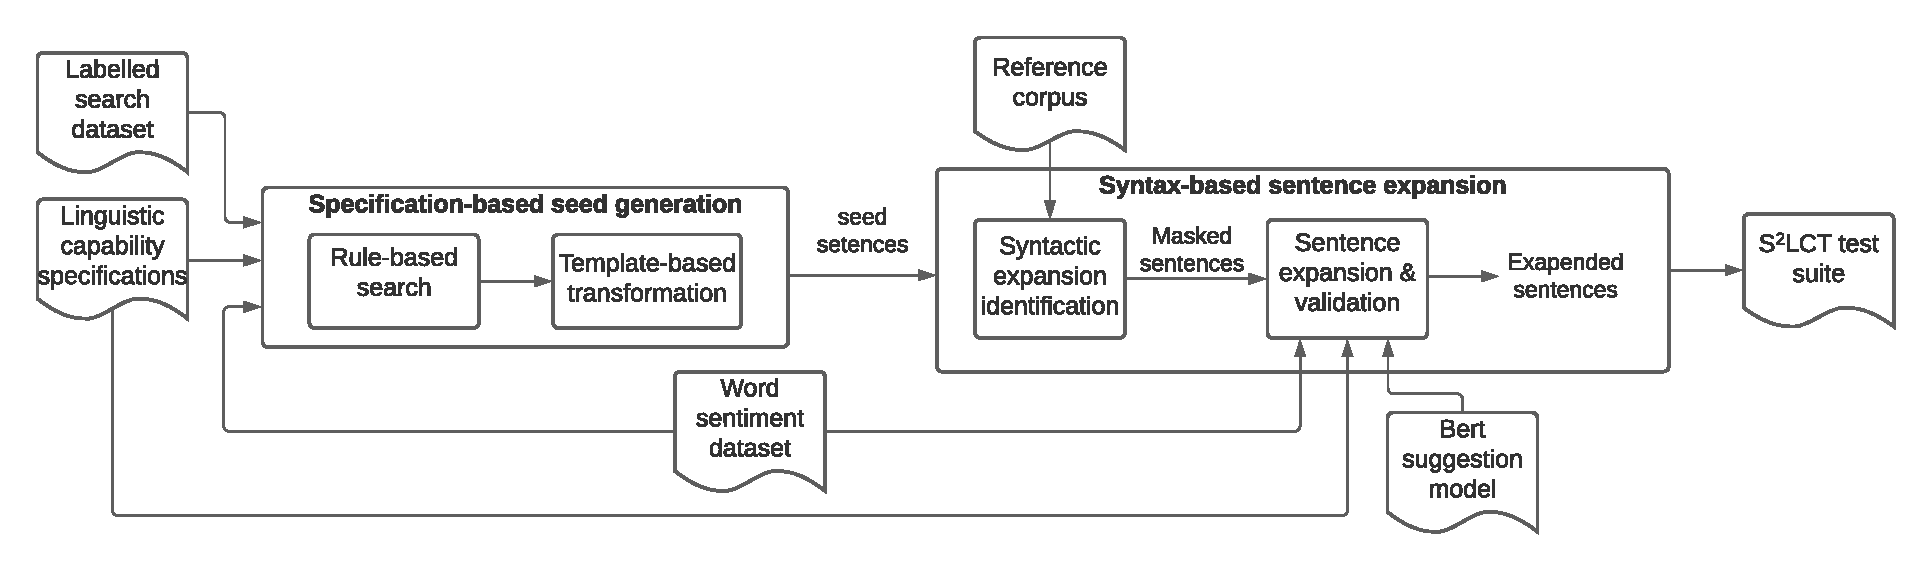
\includegraphics[width=\linewidth]{figs/overview.pdf}
  \caption{\OverviewFigCaption}
\end{figure*}

\sw{Some paragraphs in this overview part should go earlier in the
  paper. I am just writing them here for now as I don't think we have
  them in the intro/background yet.}  We design and implement
\emph{Specification- and Syntax-based Linguistic Capability Testing
  (\tool{})} to automatically generate test cases to test the
robustness of sentiment analysis models. We identify four goals for a
large and effective test suite:

\begin{description}
\item[{\bf G1}] the test suite should contain realistic \sents;
\item[{\bf G2}] the test suite should cover diverse syntactic structures;
  \item[{\bf G3}] each test case should be
categorized into a \lc;
\item[{\bf G4}] the label of each test case should be
automatically and accurately defined.
\end{description}

\Cklst's templates generate complete and realistic \sents, and each
template maps to a \lc, satisfying {\bf G1} and {\bf
  G3}. But \Cklst only uses \sw{X} manually created templates to
generate its test suite; all test cases generated by the same template
share the same syntactic structure, thus violating {\bf G2}. In
addition, the label of each \Cklst test case has to be decided
manually, associated with each template, violating {\bf G4}.

We present \tool{}, a new \lc test case generation
tool, that satisfies all of these criteria.  \sw{I could not summarize
  a cohesive idea that drives our design. Leaving it here to fill in.
  Also, I felt my writing below still lacks justification for some
  design choices (e.g., why we do the differentiation).}
Figure~\ref{fig:overview} shows the overview of \tool{}, which
consists of two phases.  The \emph{specification-based seed
  generation} phase performs rule-based searches from a real-world
dataset ({\bf G1}) and template-based transformation to obtain the
initial seed \sents.  The search rules (e.g., search for \neu
\sents that do not include any \pstv or \ngtv words) and
transformation templates (e.g., \sw{add an example} \jl{\sent
  negation}) are defined in the \emph{\lc
  specifications}, which guarantee that each resulting seed conforms
to a specific \lc ({\bf G3}) and is labelled
correctly ({\bf G4}).

The \emph{syntax-based \sent expansion} phase expands the seed
\sents with additional syntactic elements (i.e., words
\sw{more?}\jl{and production ruls in \cfg}) to cover many real-world
syntactic structures ({\bf G2}). It first performs a syntax analysis
to identify the \pos (PoS) tags that can be inserted to each
seed, by comparing the PoS parse trees between the seed \sent and
many other \sents from a large reference dataset. Each identified
tag is inserted into the seed as a \emph{mask}. It then uses an NLP
recommendation model (i.e., BERT \cite{}) to suggest possible
words. If a resulting \sent is validated to be consistent with the
specification which additionally defines the rules for expansion
(e.g., the expanded word should be \neu), {\bf G3} and {\bf G4} are
still satisfied.  Last, because some validated \sents may include
unacceptable suggested words given the context \sw{is this the
  right motivation to do selection?} \jl{I edited the \sent. please
  let me know if it is clear}, we use a heuristic (i.e., the
confidence score from the NLP recommendation model) to select the more
realistic context-aware expanded \sents into \tool{}'s test suite.

We now describe each phase of \tool{} in detail.

%\Model generates input \sents with the following phases illustrated
%in \ref{fig:OverallModel}: 1. search phase searches seed \sents
%according to its \req of \lc, 2. seed parsing phase parses the found
%seed \sents and extract their \cfg, 3. reference parsing phase
%collects \pcfg from large corpus, 4. production differentiation phase
%identifies structural expansion candidates for input expansion, and
%5.\sent selection phase generates natural expanded \sent. In this
%section, we provide more details on each phase.

\subsection{Specification-based Seed Generation}
The seed generation phase of \tool starts by searching \sents in a
real-world dataset that match the rules defined in the \lc
specification, and then transforming the matched \sents using
templates to generate seed \sents that conform to individual
\lcs. The reasons for this design choice are twofold.  First, while
generally judging which \lc any \sent falls into and which label it
should have is infeasible, there exist simple rules and templates to
allow classifying the resulting \sents into individual \lcs and
with the correct labels, with high confidence.  This enables us to
test each \lc individually.  Second, searching from a real-world
dataset ensures that the \sents used as test cases for testing \lcs
are realistic and diverse. The diverse test cases are more likely to
achieve a high coverage of the target model's functionality in each
\lc, thus detecting more errors.
%
In this phase, \tool first search and selects \sents applicable to
the \lc in a given real-world dataset with search rules. In case that
the search rules only fulfill portion of the \lc specifications, the
selected \sents are not yet appropriate to become seed, we
transform the selected \sents into seed \sents using the
heuristic templates.
%
Table~\ref{tab:specification} shows the search rules and the
transformation templates of all 11 linguistic capabilities we
implemented in \tool. The first column shows the \lc type and its
description, and the second column shows the search rule and
transformation template used in each \lc. For LC1 and LC2, the NLP
models are evaluated in the scope of short \sents with selective
sentiment words. It does not require any guidance for its
transformation because the search rule alone is sufficient to conform
to the \lcs. On the other hand, search rules of LC3 and LC4 are not is
not enough to match their \lc specification, thus \tool uses heuristic
templates to conform the found \sents to the \lc. For example, the
selected \sents becomes seeds by preturbing them with the templates
and by negating the selected demonstrative \sents to conform to LC3
and LC4 respectively (see the third and forth rows in
Table~\ref{tab:specification}).
\sw{@Jaeseong: revise the rest of 3.1 based on
  Table~\ref{tab:specification}. I commented out the old text but it
  is still in the tex file.} \jl{I revised and added the explanation}

%The search phase in \Model searches inputs in dataset and selects
%subset of input \sents in the dataset that meets the \lc
%\req. The idea behind this phase is that input distribution of
%\lc is important to generate inputs relevant to \lc. \Lc explains
%expected behaviors of NLP model on specific types of input and
%output. The NLP model is evaluated on how much it performs on the
%input and output. Thus, \lc introduces the constraints of the input
%data. Input data from the constrained distribution are only qualified
%to be used for evaluating the NLP model on the \lc.  In addition,
%diversity in inputs is important to evaluate NLP models on the
%\lc. Inputs that differ are more likely to cover the NLP model
%behavior, and more coverage increases trustworthiness of the
%evaluation. To generate inputs from same distribution on \lc and high
%diversity of inputs, we estabilish \reqs of input and output
%for each \lc, and find inputs that fulfil the \reqs. Given a
%\lc, a \req consists of search \req, transform
%\req and expansion \req. The search \req
%describes features and functionalities that we seek to have in
%inputs. \Model check each input if it satisfy the \req.

\InputWithSpace{tables/lc-requirement-table}

%\begin{figure}[t]
%  \centering
%  \lstinputlisting[language=json-pretty]{code/requirement_sa1.json}
%  \vspace{-10pt}
%  \caption{\SearchRequirementExampleFigCaption}
%  \vspace{-10pt}
%\end{figure}
%
%\begin{figure}[t]
%  \centering
%  \subfloat[][\TransformRequirementExampleSubFigCaption]{\lstinputlisting[language=json-pretty]{code/requirement_sa2.json}}
%  \\
%  \subfloat[][\TransformTemplateExampleSubFigCaption]{\lstinputlisting[language=python]{code/requirement_sa2.py}}
%  \\
%  \caption{\TransformRequirementExampleFigCaption}
%  \vspace{-10pt}
%\end{figure}
%
%Figure~\ref{fig:SearchReqEx} shows \lc of \SareqExOne. To evaluate
%this \lc, the input is required to be short and have only \neu \adjs,
%\neu \nns. In addition, the label needs to be \neu. Therefore, all
%short natural \sents with only \neu \adjs and \neu \nns are available
%to evaluate NLP models. In this work, the sentiment of the words for
%the search are classified based on the sentiment scores from
%\Swn~\cite{baccianella2010sentiwordnet}, a publicly available English
%sentiment lexicons.  It provides lexical sentiment scores and the
%sentiment word labels are categorized by implementing the rules
%in~\cite{mihaela2017sentiwordnetlabel}. Next, transform \req explains
%how the input and output needs to be tranfromed. Some \lc only accepts
%heavily limited input distribution, and it is unlikely to be included
%in searching dataset because of its high structural diversity, thus,
%finding such \sents is costly. Therefore, our approach is to find
%inputs by relaxing search requirement and transform the input to match
%the target requirement of the \lc. In this work, the inputs are
%transformed by word addition or perturbing the found inputs with \lc
%dependent templates. The figure~\ref{fig:TransformReqEx} shows the
%example of use of the template requirement. The \lc of \SareqExTwo in
%the figure~\ref{fig:TransformReqSubEx} requires inputs to be the
%negated \pstv \sents and the \neu expression in the middle. Rather
%than searching \sents that match the input distribution of the \lc,
%the \Model search \pstv and \neu inputs and combine them into negated
%\pstv \sents. Figure~\ref{fig:TransformTempSubEx} illustrates template
%for the \lc. According to the \lc, The value of ``sent1'' and
%``sent2'' become each searched \neu and \pstv inputs respectively, and
%the template completion generates new inputs that matches the target
%\lc. In addition, the transformation of inputs also produce high
%diversity in the inputs because of that from initially found
%inputs. In this paper, we will denote the searched inputs in this
%phase as seed inputs.

\subsection{Syntax-based \Sent Expansion}

The simple search rules and transformation templates used to generate
the seed \sents may limit the syntactic structures these seeds may
cover. To address this limitation, the syntax-based \sent expansion
phase extends the seed \sents to cover syntactic structures
commonly used in real-life \sents. Our idea is to differentiate the
parse trees between the seed \sents and the reference \sents
from a large real-world dataset. The extra PoS tags in the reference
parse trees are identified as potential syntactic elements for
expansion and inserted into the seed \sents as masks. We then use
masked language model to suggest the fill-ins. If the resulting
\sents still conform to the \lc specification,
they are added to \tool{}'s test suite. \sw{May have some redundancy
  and inconsistency with the overview part.}

\subsubsection{Syntax Expansion Identification}

Algorithm \ref{alg:diff} shows how masks are identified for each seed
\sent.  It takes the parse trees of the seeds, generated by the
Berkeley Neural
Parser~\cite{kitaev2018seedparser,kitaev2019seedparser}, and a
reference context-free grammar (CFG) from the Penn Treebank corpus
dataset \cite{} as inputs.  The reference CFG is learned from a large
dataset \cite{} that is representative of the distribution of
real-world language usage.  The algorithm identifies the discrepancy
between the seed syntax and the reference grammar to decide how a seed
can be expanded.
%This phase builds \pcfg from the reference corpus. \cfg
%is constructed by parsing \sents in the corpus and extracting
%\prodrs. In addition, the probability of \cfg is estimated by
%its frequency over corpus. The output of this phase is the constructed
%\pcfg, and it is compared with seed parse trees. For our
%implementation, we build the \pcfg from the Penn Treebank corpus dataset.


%\paragraph{Seed parsing.}
%To expand seed \sent and generate fluent and faithful \sent
%used for evaluation, \Model studies structure of each seed input for
%its expansion.
%Seed parsing takes each seed as
%input, and outputs its parse tree of the seed, using the Berkeley Neural
%Parser~\cite{kitaev2018seedparser,kitaev2019seedparser}.

%\paragraph{Reference parsing.}
%We take a large-scale real-world dataset as reference for \sent expansion.

\begin{algorithm}
  \caption{\ProdDiffAlgCaption}
  \begin{algorithmic}[1]
    \State \textbf{Input:} Parse trees of seed sentences $\textbf{S}$,
    reference \pcfg$\textbf{R}$
    \State \textbf{Output:} Set of expanded masked sentences $\textbf{S\_exp}$
    \For {$seed$ from $S$}
      \For {each production rule $seed\_prod$ from $seed$}
        \State $seed\_lhs = seed\_prod.lhs$
        \State $seed\_rhs = seed\_prod.rhs$
        \For {$ref\_rhs$, $ref\_prob$ from $R[seed\_lhs]$}
          \If {$seed\_rhs$ is superset of $ref\_rhs$}
            \State $parent = seed\_prod.parent$
            \State $prob = ref\_prob$
            \While {$parent$ is not empty}
              \For {$par\_rhs$, $par\_prob$ from $R[parent.lhs]$}
                \If {$parent.rhs == par\_rhs$}
                  \State $prob = prob \cdot par\_prob$
                  \State $parent = parent.parent$
                  \State break
                \EndIf
              \EndFor  
            \EndWhile
            \State $P.add([seed\_prod, ref\_prod, prob])$
          \EndIf
        \EndFor
      \EndFor
      \If {$P$ is not empty}  
        \State Select Top-k $ref\_prod$ along with probabilities in P
        \For {each $seed\_prod$, $ref\_prod$ in the Top-k selected P}
          \State replace $seed\_prod$ with $ref\_prod$ in $seed$
          \State replace expanded component in $ref\_prod$ with $MASK$
          token in $seed$ sentence
          \State $S\_exp.add([ref\_prod, expanded sentence])$
        \EndFor
      \EndIf
    \EndFor
  \end{algorithmic}
\end{algorithm}


For each production of in each seed's parse tree (lines 3 and 4), we
extract its non-terminal at the left-hand-side (line 5), $s\_lhs$, and
the grammar symbols at the right-hand-side (line 6), $s\_rhs$. In line
7, the algorithm iterates through all productions in the reference
context-free grammar and match these that have the same non-terminal
at the left-hand-side as $s\_lhs$.  The right-hand-side of each
matched production is called $r\_rhs$.  If $s\_rhs$ consists of a
subset of the grammar symbols in $r\_rhs$ (line 8), the additional
symbols in the $r\_rhs$ are inserted as masks in the parse tree of
seed \sent, in their respective positions in the expanded production.
The left to right traversal of the leaves of an expanded parse tree
forms a masked \sent.  Lastly, due to the inefficient cost of
accessing full list of the masked \sents, we randomly select $k$
masked \sents for the next \sent expansion and validation phase when
the masked \sents are more than maximum number of masked \sents. The
random sampling is unbiased approach since it gives same chance to be
chosen. Thus, the random sample becomes representative of the
population of the masked \sents, and it efficiently shows the
usefulness of the \tool.  \sw{Add justification: why we need to select
  k masked \sents (performance?)  and why random makes sense.} \jl{I
  added the statement for it}

\begin{figure*}[t]
  \centering
  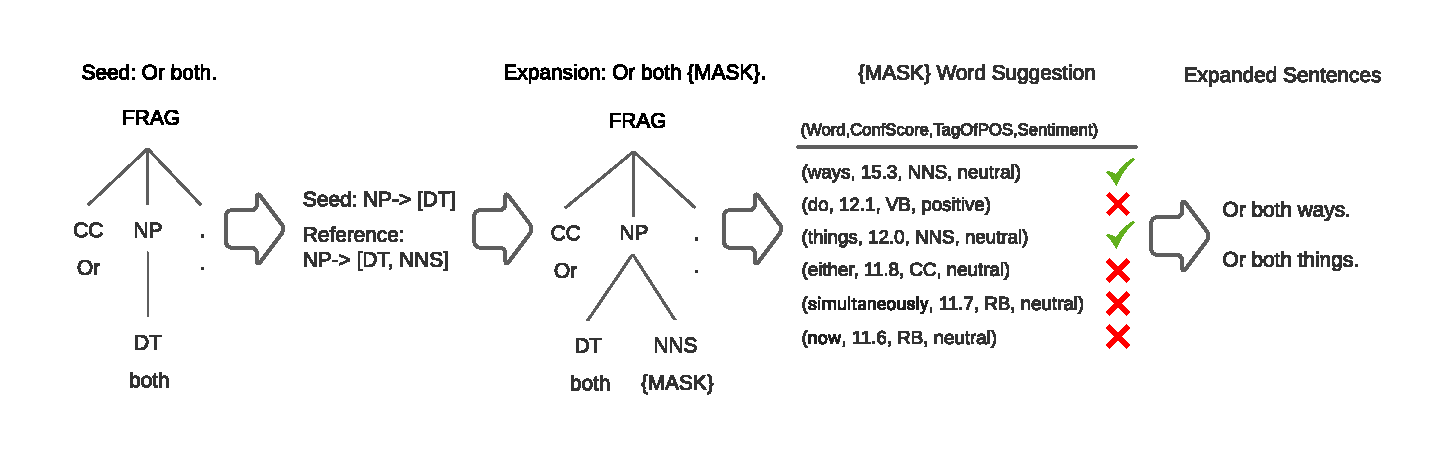
\includegraphics[scale=0.7]{figs/running_example.pdf}
  \caption{\RunningExCaption}
%  Expansion of the seed \sent ``Or
%both.''. For a \prodr in seed ``NP->[DT]'' on the left, the \prodr of
%``NP->[DT, NNS]'' is found in reference. Thus, the component NNS can be expanded in the
%seed and ``NP->[DT]'' is replaced with ``NP->[DT, NNS]'' and it generates new
%expanded \sent on the right.
\end{figure*}

\paragraph{Running example.} Figure~\ref{fig:ExpEx} shows an example using Algorithm \ref{alg:diff}
to generate a masked \sent. The \sent ``Or both." is a seed of \lc of
\SareqExOne.  The tree on the left shows the parse tree of this seed;
it consists of two productions: ``FRAG->[CC, NP, .]" and ``NP->[DT]".
When matching the left-hand-side non-terminal of the second production
(i.e., ``NP") in the reference CFG, we found that it includes a
production ``NP->[DT, NNS]" which has an additional symbol ``NNS" on
the right-hand-side.  The algorithm thus expands the parse tree with
this symbol, shown in the second tree.  The masked \sent ``Or both
\{MASK\}." is the result of the left-to-right traversal of this
expanded parse tree.

%Given the seed parse tree and reference \pcfg, production
%differentiation phase suggests structural expansion candidates on the
%seed input. this phase aims to analyze which structural components and
%where they can be added into the seed structure for its expansion. To
%do so, we explore reference \prodrs comparing it with each \prodr used
%in seed input. This results in the phase described in
%Algorithm~\ref{code:ProdDiffAlg}. For each production rule in seed
%inputs ($seed\_prod$), it searches production rules in reference
%($ref\_prod$) which it has same non-terminal on the \lhs
%($seed\_prod.lhs==ref\_prod.lhs$) and superset of \rhs of the seed
%production rule ($seed\_prod.rhs \subset ref\_prod.rhs$).  As we
%assume that the reference \cfg is built from real world data
%distribution, the elements in the complement set ($ref\_prod.rhs -
%seed\_prod.rhs$) become an expansion candidate which can be expanded
%from the $seed\_prod.rhs$ found in real world. In addition, the
%measure of how consistent the production rule is with the given seed
%structure is given in its probability of the reference production rule
%($ref\_prob$) multiplied by that of parents of $seed\_prod$. The
%expansion candidate consists of terminal or nonterminal symbols. When
%there is a phrase-level or clause-level nonterminal symbol, \eg noun
%phrase, it needs to be expanded and replaced with word-level
%nonterminal or terminal symbols to generate the expansion
%candidate. The number of feasible replacement is unbounded because of
%its high degree of freedom. Therefore, in this work, we focus on the
%expansion candidate with only the word-level nonterminal or terminal
%symbols for the effectiveness of \Model. Lastly, the expanded
%component is replaced with the mask token for the next phase. The
%example of the expansion is illustrated in
%Figure~\ref{fig:ExpEx}. The ``NP->[DT]'' is queried into
%reference, and ``NP->[DT,NNS]'' is identified as its expansion
%candidate since the \rhs of ``NP->[DT,NNS]'' is superset of that of
%``NP->[DT]''. the component of NNS is replaced with mask token in
%\sent-level. Therefore, the ``Or both \{MASK\}.'' is suggested for
%the next phase.

\subsubsection{\Sent Expansion and Validation}

In this phase, the words to fill in the masks in the masked \sents are
suggested by the BERT pretrained model~\cite{devlin2019bert}.  The
BERT is a transformer-based \nl model. It is pretrained on two tasks
of masked token prediction and next sentence prediction. As a result
of the training process, the BERT model suggests word for the mask
token according to its surrounding context in \sent. For each masked
token, multiple words are suggested ranked by their confidence scores.
\sw{Algorithm 1 does not require we only have one mask in the masked
  \sent. Can the model suggest multiple words at the same time?}
\jl{yes. it can predict multiple masked tokens at the same time.}
\sw{Say a bit more about the BERT model suggestion. E.g., it may
  suggest multiple words for the same mask but they are ranked?}
\jl{I added the explanation of BERT}
%
Because BERT model is not aware of the \lc
specification and the grammar symbol in the expanded parse tree, an
expanded \sent using the suggested words may no longer satisfy the
\lc specification. Therefore, we perform validation
on the suggested words and only accept them if the following three
criteria are met.

First, the PoS tag of the suggested word must match the PoS tag of the
expanded symbol in the parse tree. For the example in
Figure~\ref{fig:ExpEx}, the masked symbol is a ``NNS" (i.e., plural
noun); thus, the suggested word must also be a ``NNS". In this work,
we use \spacy, a free open-source library for \nlp, for extracting PoS
tags for each suggested word.\sw{Say how we obtain the PoS tag of a
  suggested word.}\jl{I added it} Second, it is required that the
sentiment of the expanded \sent becomes the same as the seed \sent. To
ensure this, the suggested words must be \neu.  \sw{Should we present
  this as part of specification, called expansion rule?} \jl{I did it
  because I think that there is no issue on mentioning it and that is
  how we assumed and did} Third, we additionally verify that the
expanded \sents satisfied the same search rules for the seed
\sent. Our goal for generating the expanded \sents is to use them for
evaluating the \sa models on the associated \lc in addition to the
seed \sent. It is only achieved when the expanded \sents are also met
with the same search rules for the \lc. For LC1 as an example, the
expanded \sent must still conform to the specification of the seed's
\lc specification. Therefore, the expanded \sents are required to be
short and to only have \neu adjectives and \nns. \sw{Say why we use
  the third criteria only for LC1 and LC2.}  \jl{I added the
  explanation}

\paragraph{Running example.} The third step in Figure~\ref{fig:ExpEx} shows the words suggested
by BERT. For this masked \sent, BERT suggested six words. Each word
is associated with the confidence score provided by BERT, the PoS tag,
and the sentiment. Among the six words, only ``ways'' and ``things''
are validated by \tool{} because they have the Pos tag ``NNS'' and are
\neu. In addition, it is found that both \sents meets the search
rule of the associated \lc of \SareqExOne. In the end, two \sents
of ``Or both ways'' and ``Or both things'' are generated.  \sw{Do we
  also check if the expanded \sent meets the
  specification?}\jl{Yes. I added the explanation of validation of \lc
  \req}

%The suggested word are
%validated by three criteria. First, The tag of POS must be matched with
%that suggested from the production differentiation phase. In the
%example in the Figure~\ref{fig:ExpEx}, the mask token comes from the
%structural component of NNS, plural noun. Therefore, the BERT
%suggested words must be also tagged with the NNS. Accordingly, every
%words of the NNS are only available. Second, \Model focuses on the \sa
%task, and it assume that the suggested words must not change sentiment
%of its input and must preserve its consistency of original sentiment
%label. Therefore, we only accept the \neu words for the
%expansion. Third, the expanded \sents with the BERT suggested words
%must be appropriate for evaluating NLP models on the target \lc, and the
%\sents must pass the \req of the \lc. In this work, the BERT
%suggestions are validated by the three criteria.

\subsubsection{\Sent Selection}
\sw{@Jaeseong: Add how we select expanded \sents and motivate why.}
After 
\paragraph{Running example.} \sw{Refer to the example to say how we
  use the BERT score to select.} \jl{I dont think we need this
  subsection of \sent selection it is already explained at the
  previous stage with running example.}

%\section{Research questions for evaluation}
\label{sec:rq}

\section{Experiment}
\label{sec:experiment}
%
In this section, we present experiments to evaluate the effectiveness
of our proposed evaluation methodology. In particular, we address the
following research questions:

\begin{enumerate}[label=\textbf{RQ\arabic*}]
\item \label{rq:one}: How effective is our proposed evaluation model
  for finding failures given a linguistic capability?
\item \label{rq:two}: How effective is our proposed model for
  generating diverse test cases? % self bleu score
\item \label{rq:three}: How effective is test cases generated from our
  proposed model for detecting diverse type of errors? % retraining
  acc score
\item \label{rq:four}: How effective is our new test case generation
  using \cfg expansion? % ablation study
\end{enumerate}

For answering \ref{rq:one} and \ref{rq:two}, we generate test cases
and use them for evaluating model on linguistic capabilities. In this
experiment, We assess the ability to find failures by anlyzing model's
performance on the generated test cases. We also measure the diversity
among the generated test cases using similarites among them. Next, we
answer \ref{rq:three} by retraining \sa model with generated test
cases and measuring performances. The idea behind this is that more
comprehensive inputs becomes closer to real-world distribution and
addresses more type of errors.  Therefore, it leads to improve the
model performance. In this experiment, We retrain the model and
compare performances of the retrained model. Not only that, we conduct
ablation study of \cfg expansion to understand the its impact in our
approach.

\subsection{Experiment Setup}
%
\MyPara{Seed Input Selection}
%
For each linguistic capability, we first search all sentences that
meet its requirement. Among found sentences, we randomly select 10
sentences due to memory constraint.

\MyPara{Word Sentiment}
%
we extract sentiments of words using the
\Swn~\cite{baccianella2010sentiwordnet}. The \Swn is a publicly
available lexical resource of words on Wordnet with three numerical
scores of objectivity, positivity and negativity. Sentiment word
labels from the scores are classified from the algorithm from Mihaela
\etal~\cite{mihaela2017sentiwordnetlabel}.

\MyPara{\Cfg Expansion}
%
We build a reference \Cfg of natural language from the English Penn
\Trb corpora~\cite{mitchell1993treebank,nltkTreebankCorporaWebPage}.
The corpus is sampled from 2,499 stories from a tree year \Wsj
collection The \Trb provides a parsed text corpus with annotation of
syntactic and semantic structure. In this experiment We implement the
\trb corpora available through \Nltk, which is a suite of libraries
and programs for \Nlp for English. In addition, we parse the seed
input using into its CFG using the Berkeley Neural
Parser~\cite{kitaev2018constituency, kitaev2019multilingual}, a
high-accuracy parser with models for 11 languages. The input is a raw
text in natural language and the output is the string representation of
parse tree. Next after comparing CFGs between reference and seed input,
we randomly select 10 expansions for generating templates due to
memory constraint.

\MyPara{Synonyms}
%
\Model searches synonyms of each token from synonym sets extracted
from \Wrdnt using \Spacy open-source library for NLP.

\MyPara{Models}
%
We evaluate the following \sa models via \Model:
\Bert~\cite{devlin2019bert}, \Roberta~\cite{liu2019roberta} and
\Dbert~\cite{sanh2019distilbert}. These models are fine-tuned on \Sstt
and their accuracies are \BertAcc, \RobertaAcc and \DbertAcc.

\MyPara{Retraining}
%
We retrain \sa models. we split \Model generated test cases into
train/validation/test sets with the ratio of 8:1:1. The number of
epochs and batch size for retraining are 1 and 16 respectively.

\section{Experimental Results}
\label{sec:result}

This section presents the experimental results and the answers to the RQs. More results are available at https://github.com/csresearcher27/s2lct$\_$project.

% \InputWithSpace{tables/test-results-table}
%% \InputWithSpace{tables/test-results-3-50-table}
% \InputWithSpace{tables/test-results-3-100-table}
% \InputWithSpace{tables/test-results-3-200-table}
\InputWithSpace{tables/test-results-all-table}
\InputWithSpace{tables/test-results-hs-table}


\begin{figure}
    \centering
    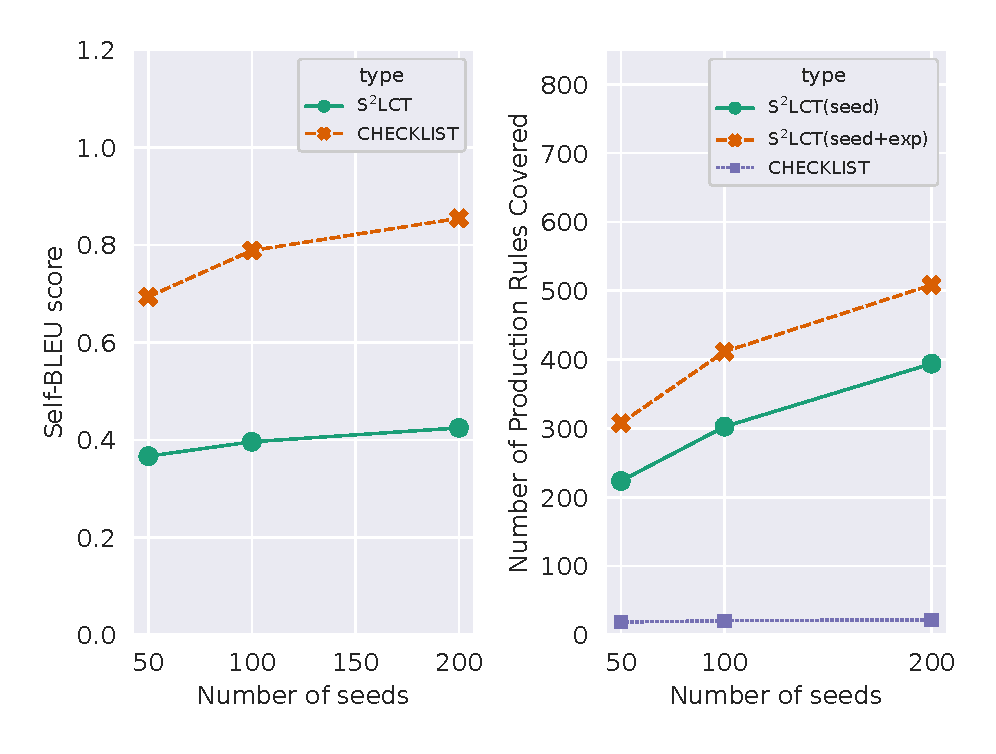
\includegraphics[width=0.35\textwidth]{figs/pdr-selfbleu-agg-lineplot.eps}
    \caption{\PdrSelfbleuFigCaption}
\end{figure}

% \begin{figure}%
%     \centering
%     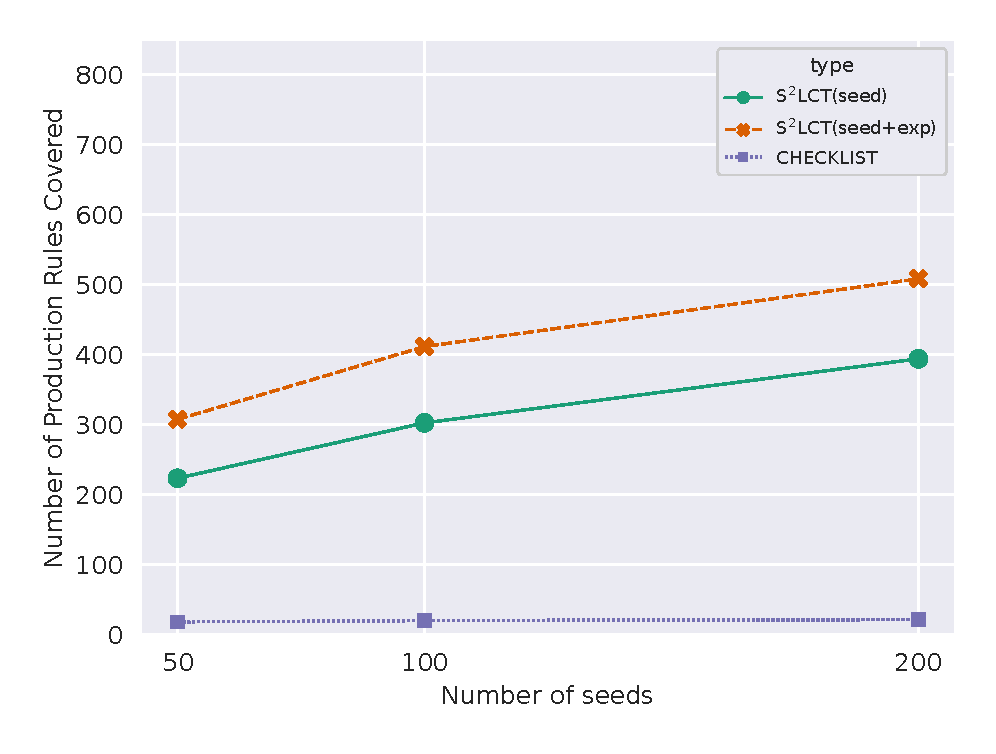
\includegraphics[width=0.35\textwidth]{figs/pdr-agg-lineplot.eps}
%     \caption{\PdrFigCaption}
% \end{figure}


% \begin{figure}%
%     \centering
%     \subfloat[][\centering\SelfbleuFigCaption]{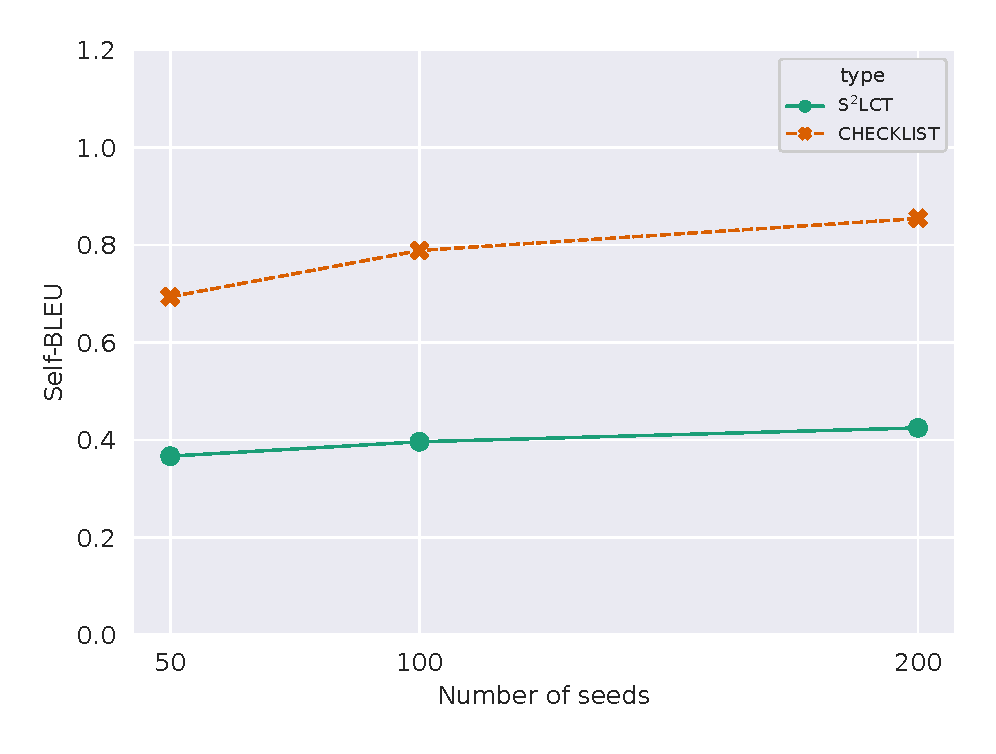
\includegraphics[width=0.35\textwidth]{figs/selfbleu-agg-sample-lineplot.eps}}%
%     \qquad
%     \subfloat[][\centering\PdrFigCaption]{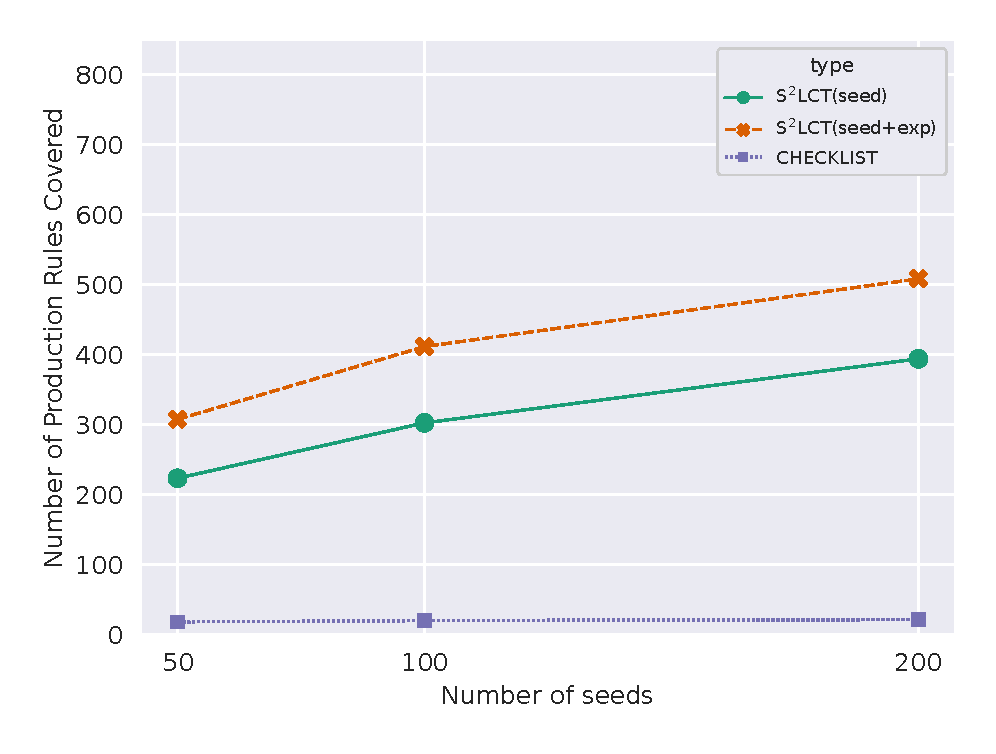
\includegraphics[width=0.35\textwidth]{figs/pdr-agg-lineplot.eps}}
%     \caption{\FailModelsFigCaption}
% \end{figure}

\begin{figure}%
    \centering
    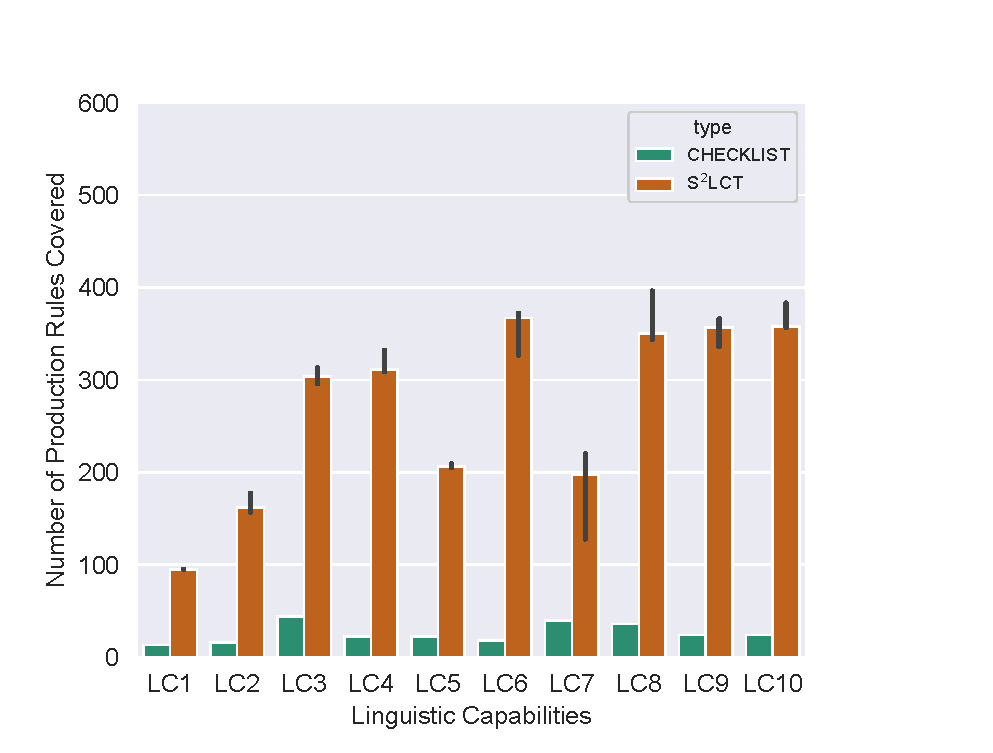
\includegraphics[width=0.35\textwidth]{figs/pdr-ours-50seeds-barplot.eps}
    \caption{\PdrBarplotFigCaption}
\end{figure}

\begin{figure}%
    \centering
    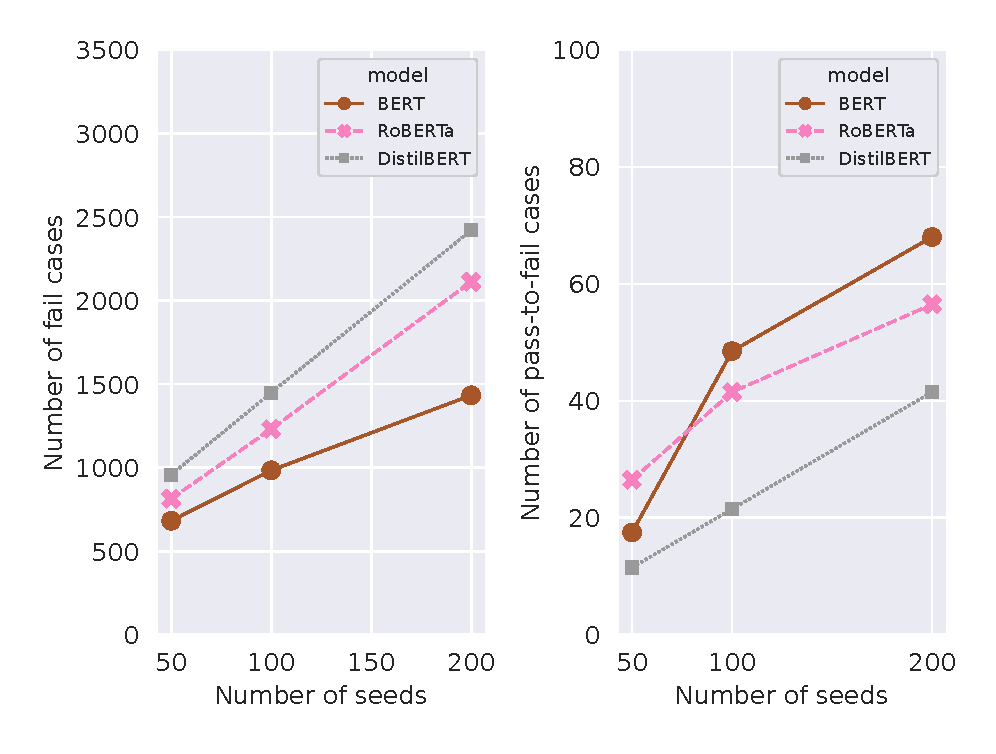
\includegraphics[width=0.35\textwidth]{figs/numfail-pass2fail-agg-lineplot.eps}
    \caption{\FailModelsFigCaption}
\end{figure}

% \begin{figure}%
%     \centering
%     \subfloat[][\centering\NumFailModelsSubFigCaption]{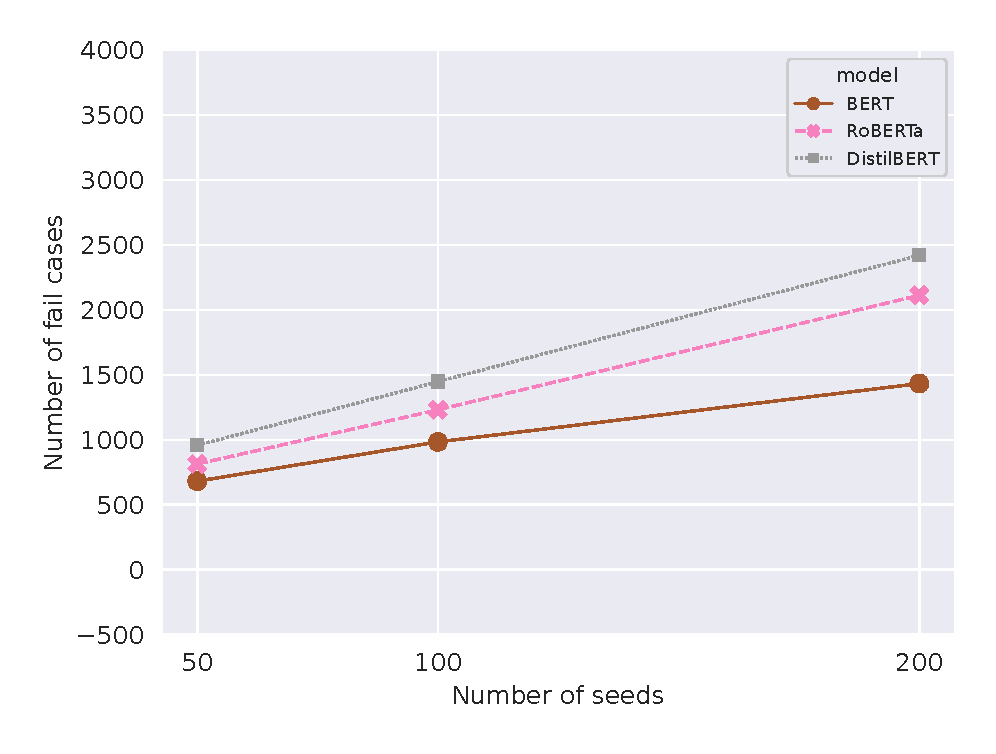
\includegraphics[width=0.35\textwidth]{figs/numfail-agg-lineplot.eps}}%
%     \qquad
%     \subfloat[][\centering\FailRateModelsSubFigCaption]{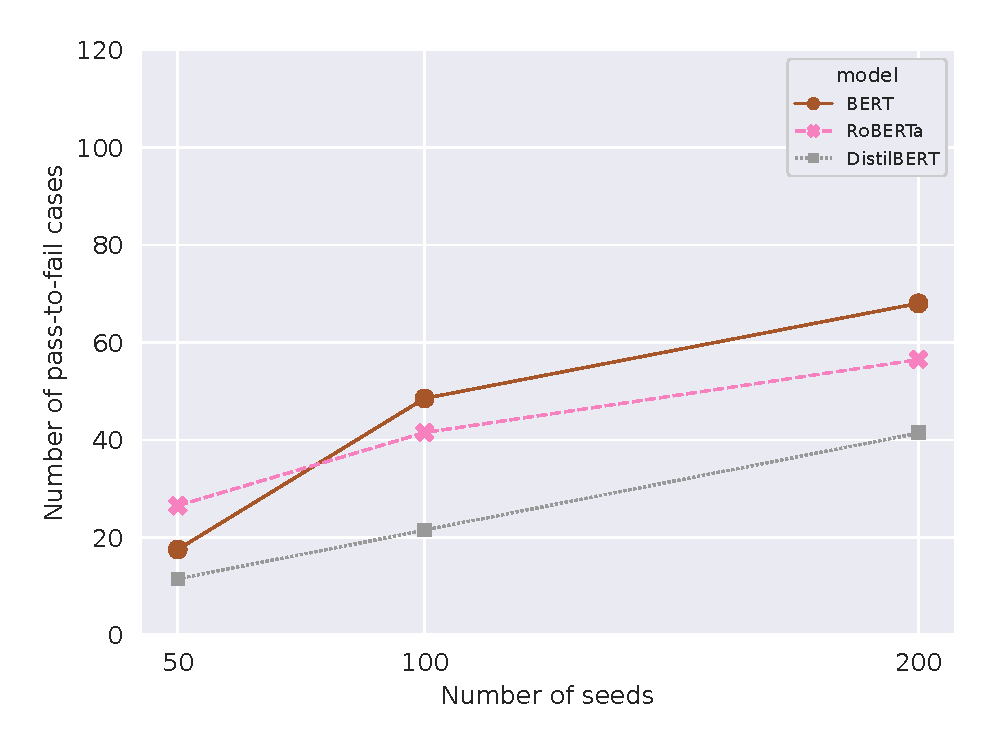
\includegraphics[width=0.35\textwidth]{figs/pass2fail-agg-lineplot.eps}}
%     \caption{\FailModelsFigCaption}
% \end{figure}

\subsection{RQ1: Test Case Diversity}

Our results show that \emph{\tool generated many test cases that the sentiment analysis models failed to predict the correct labels, and it produced significantly more diverse test cases than \Cklst did.}

\paragraph*{\selfbleu} Left in Figure~\ref{fig:PdrSelfbleu} compares the \selfbleu scores between \tool seed sentences and \Cklst test cases. The x-axis shows sizes of random samples of \tool seeds and \Cklst test cases, and y-axis shows the \selfbleu scores.
% Median value of \selcbleu scores are computed from randomly sampled seeds over 3 trials for each \lc,
Median of the \selfbleu scores over all \lcs is shown in left in figure \ref{fig:PdrSelfbleu}. We observe that \selfbleu scores of \Cklst test cases is significantly higher than those of \tool seeds, for all numbers of seeds. This result indicates \Cklst test cases are less diverse than \tool seeds, which demonstrates the benefit of searching from a real-world search dataset over creating test cases from limited number of preset templates.
% From the figure, we can observe that seed generation step in \tool generates more diverse text sentences than \Cklst.

\paragraph*{\Pdr} Right in figure~\ref{fig:PdrSelfbleu} compares \pdr between the \tool seed sentences, \tool seed and expanded sentences, and the \Cklst test cases. The x-axis shows the sizes of random samples of \tool seed sentences, \tool seed and expanded sentences, and \Cklst test cases, and y-axis shows the \pdr scores. Median of the \pdr scores over all \lcs is shown in the right in the figure~\ref{fig:PdrSelfbleu}. The figure \ref{fig:PdrSelfbleu} shows that \tool seed and/or expanded sentences produce significantly higher \pdr scores than \Cklst test cases did. Also, more \tool seeds cover more production rules.

Figure~\ref{fig:PdrBarplot} compares the \pdr between 50 \tool seeds and all \Cklst test cases for each \lc. The x-axis shows each one \lc, and the y-axis is the \pdr for these test cases.
% \tool test cases are generated from randomly selected 50 seeds, and the median value over 3 trials for each \lc is reported.
% It is observed that \tool covers significantly higher number of different syntactic production rules than \Cklst for all \lcs.
We observed that even with only 50 seeds in each \lc, \tool seeds cover significantly higher number of production rules than all \Cklst test cases (ranging from 95 for LC1 to 367 for LC6 for \tool seeds and from 13 for LC1 to 44 for LC3 for \Cklst seeds) in each \lc.
% (ranging from 4.92 times to 20.38 times higher scores for LC7 and LC6 respectively) 

Overall, the above results show that \tool test cases are significantly more diverse in terms of syntactic structure than \Cklst.

\paragraph*{Model Test Results} Table~\ref{table:TestResult} shows the testing results of the three NLP models on \tool test cases using 50 seeds. First column lists linguistic capabilities for the \sa task, and Column 2 shows the numbers of seed test cases, and Column 3 shows the median numbers of expanded test cases over 3 trials. Columns 4 and 5 show the median numbers of failed test cases and the failure rates (i.e., percentage of test cases that a model predicts incorrect labels) of each NLP models on the seed and expanded test cases over the 3 trials, respectively. Column 6 shows the median number of expanded test cases that failed, but their corresponding seed test cases passed over the 3 trials(\Ptf). We observe that in all \lcs, \tool produces hundreds of test cases, expanding at least an order of magnitude more test cases than the seeds. LC1 and LC5 have 19 and 26 seeds, respectively. This is because \tool's search rules and transformation templates of these two linguistic capabilities produced few seeds. Nevertheless, the syntax-base sentence expansion phase generated of 224 and 1090 test cases, respectively.
In terms of model performance, all three models achieve low failure rates in LC2 and LC9 while the failure rates are high in all other linguistic capabilities (13.52\%-99.95\%). We also observe that there are many expanded test cases that failed, but their corresponding seeds did not (last column). This shows that the syntax-based sentence expansion phase indeed introduces more diverse sentence structures in the test cases that cause the models to fail.

In addition, Figure~\ref{fig:FailModels} shows the numbers of fail and pass-to-fail cases with different number of seeds used. We observed that more \tool seeds introduce more failed cases and more \Ptf cases, demonstrating the benefit of using more seeds when resource permits.



\begin{figure}
    \centering
    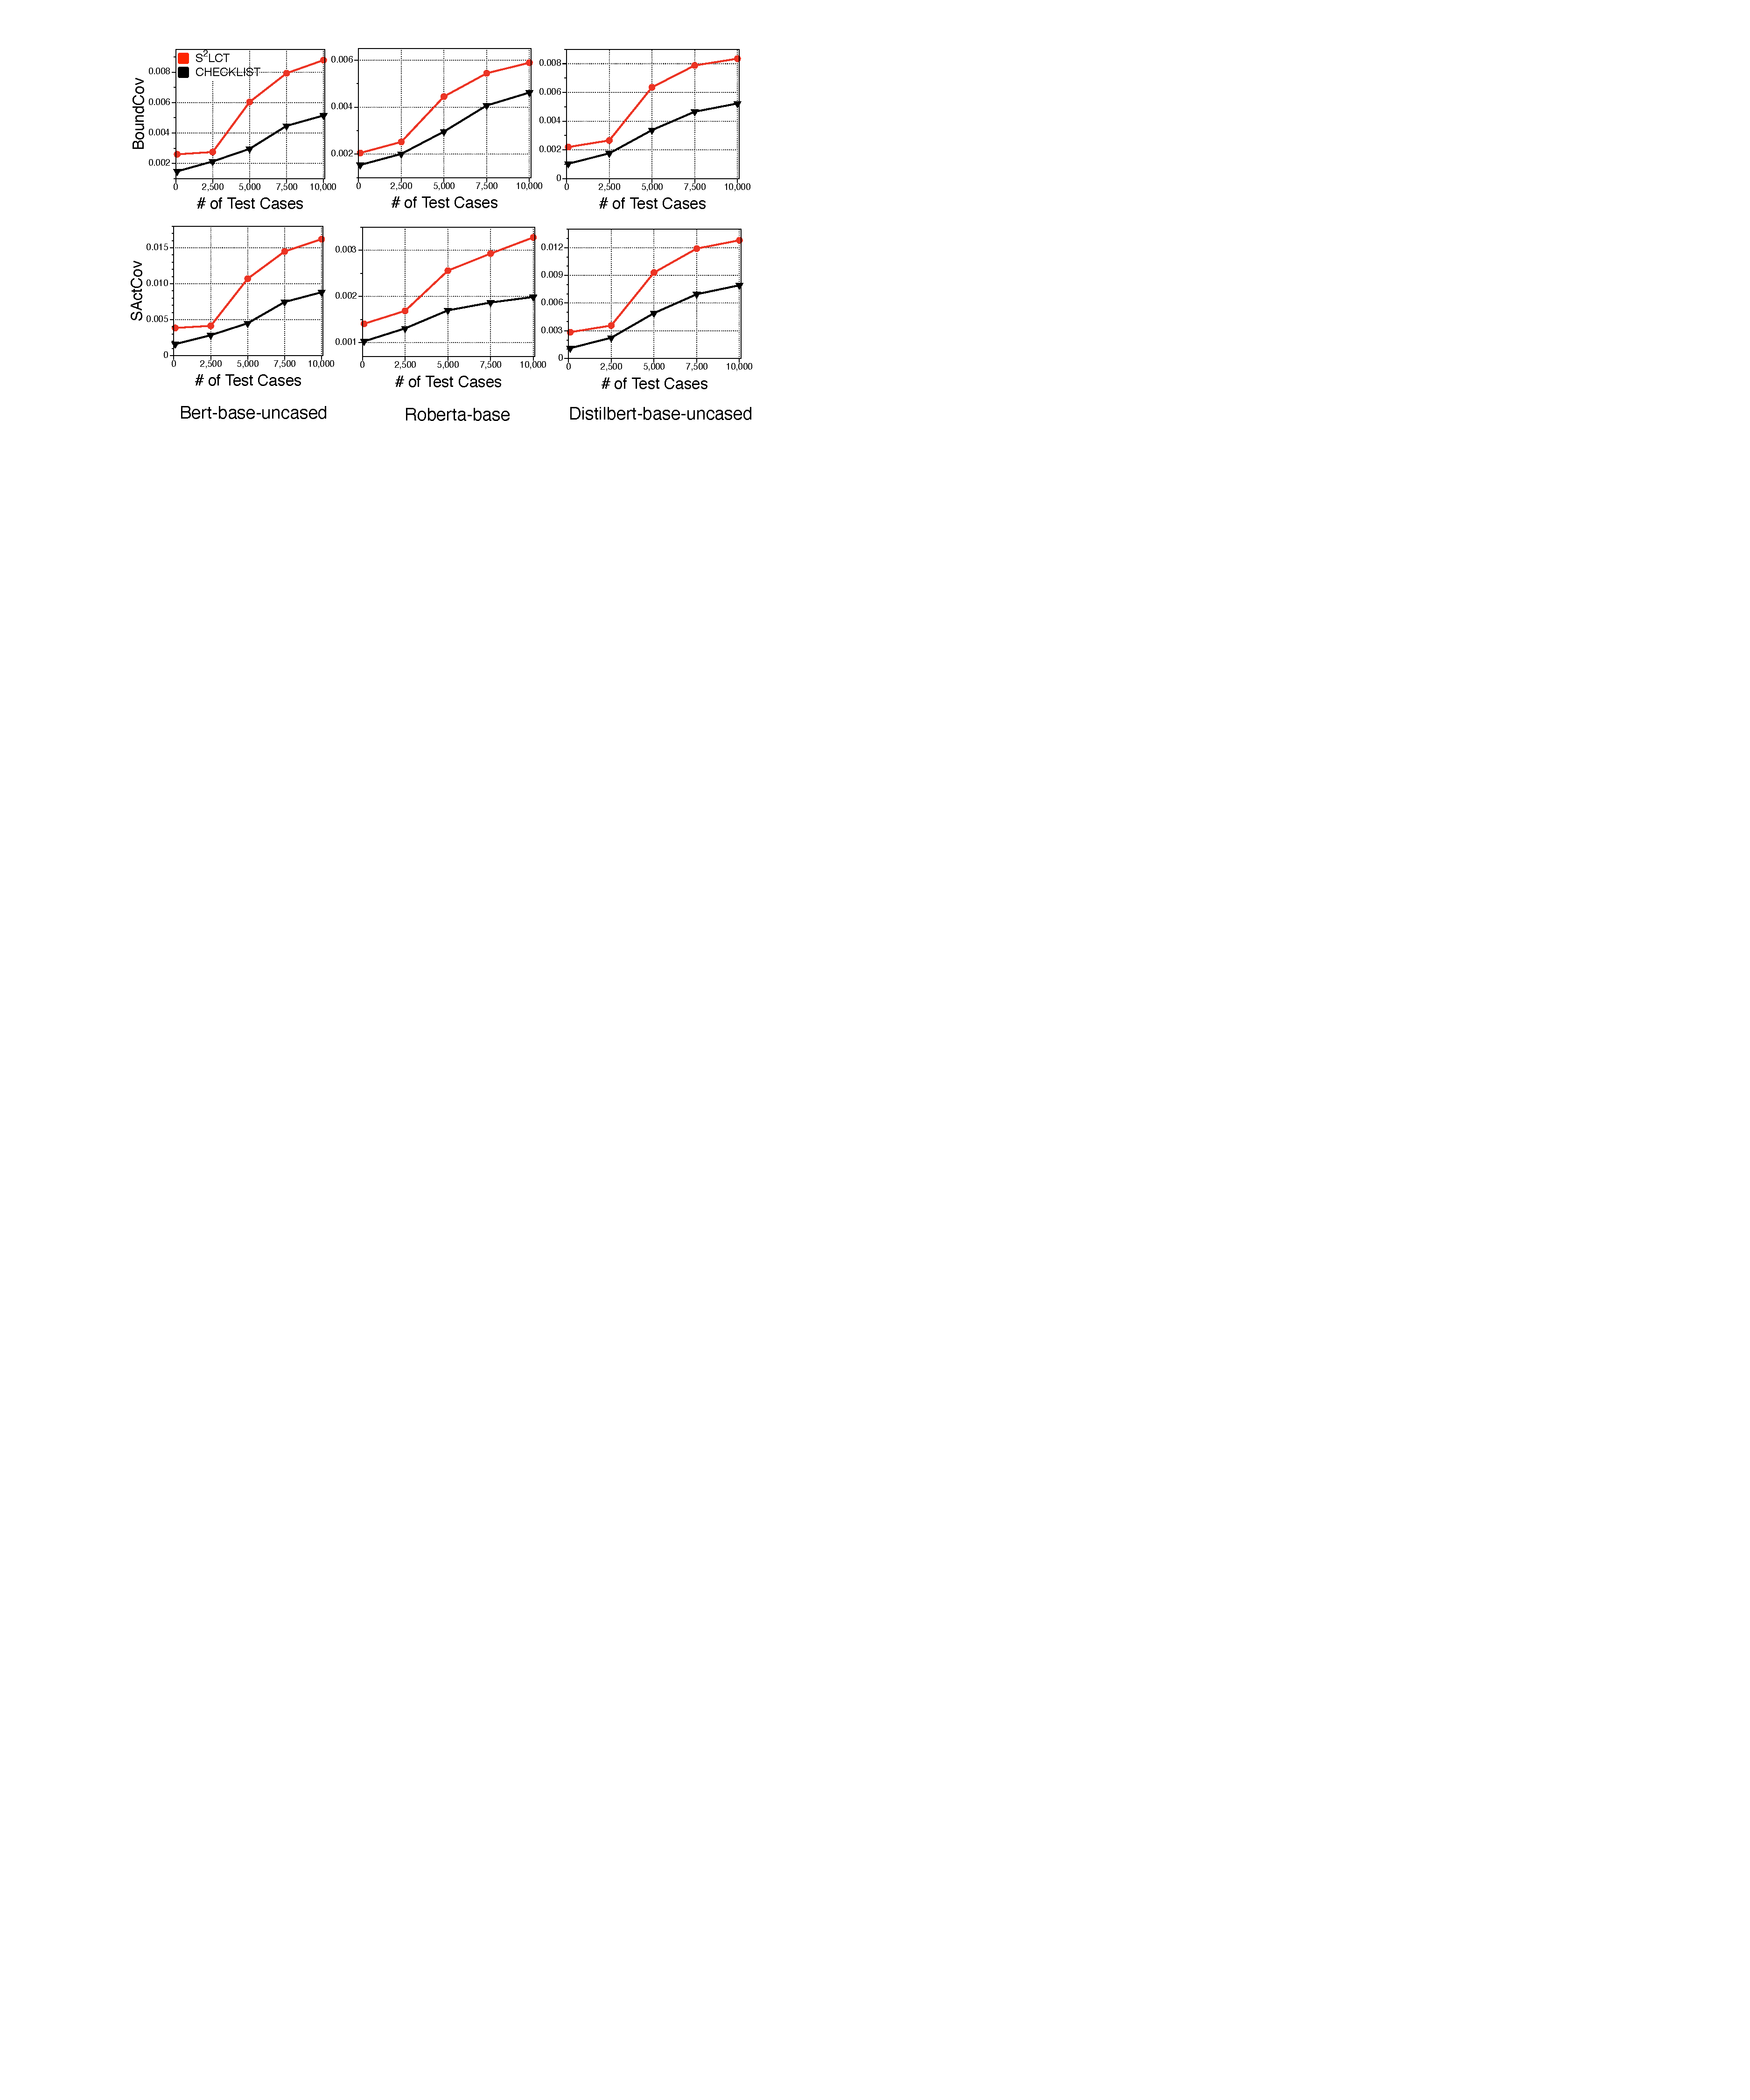
\includegraphics[width=0.5\textwidth]{figs/coverage.pdf}
    \vspace{-4mm}
    \caption{Coverage results of \tool and \Cklst test cases.}
    \label{fig:coverage}
\end{figure}

Next, Figure \ref{fig:coverage} shows the coverage results of \tool and \Cklst test cases. The red line represents \tool coverage and the black line represents \Cklst coverage. Each column in Figure \ref{fig:coverage} represents the results for one NLP model. The first row is the \textit{BoundCov} results and the second row is the \textit{SActCov} results.

We made three observations.
First, for \emph{all} experimental settings (i.e., NLP model and coverage metric), \tool achieves higher coverage than \Cklst. Recall that a higher coverage implies the test cases are more diverse and do not have a similar statistical distribution to the model training data. As a result, a test suite with greater coverage complements the model training data distribution (\ie holdout testing data) better.
For example, for the first NLP model under test, \tool can achieve a higher coverage than \Cklst with only half the number of test cases.
This result confirms that \tool can generate more diverse test cases to complement the holdout dataset for testing NLP models.

Second, as the number of test cases increases, the test suite can achieve better coverage. Such observation is intuitive. However, generating a more extensive test suite is not easy, particularly  for \Cklst, which is a manually template-based approach.

Third, for each NLP model, there is no fixed relationship between \textit{BoundCov} and \textit{SActCov}. In other words, while a test suite may produce higher \textit{BoundCov} for some models, the same test suite may get higher \textit{SActCov} for other NLP models.
Recall that \textit{BoundCov} measures both the upper and lower corner neurons and \textit{SActCov} measures only the upper corner neurons. 
Such observation implies that the upper and lower corner neurons are distributed unevenly, and measuring only one of them is not enough.

\InputWithSpace{tables/manual-study-table}

\subsection{RQ2: Correctness of Sentiment Labels}
Table~\ref{table:ManualStudy} shows results of our manual study. The first column distinguishes the seed and expanded sentences. The number of test cases used for the study is represented in the
second column. The label consistency score defined
in Equation~\ref{metric:srel} is shown in column 3.

We observe that \emph{\tool generates test cases that consistently
  label their sentiment correctly.}  Column 3 shows that the label
consistency scores are 0.83 and 0.84 for the seed and expanded
sentences, respectively.
This means that \tool generates test oracles consistent with
human understanding most of the time. Also, there is
little difference of the scores between the seed and expanded
sentences. This implies that the syntax-based sentence expansion in
\tool preserves the sentiment as its seed.

% \sw{This paragraph is problematic. We are saying the inconsistency is just caused by human, indicating our tool is always correct?} Nevertheless, there exist inconsistency between \tool and manual labels. The causes of inconsistency are twofold. First, complicated sentences have led the participants to
% misunderstand its meaning. Second, phrase in a sentence has
% multiple interpretations of its sentiment. For example, the
% word ``easy'' could be interpreted as both compliment and back-handed
% insult.  
%% \sw{What are
%%   the causes of inconsistency? Looks like the main source of
%%   inconsistency comes from seed generation? Any insights on how it
%%   happened (e.g., issue with original labels, search rules, or
%%   templates?}

\subsection{RQ3: Correctness of Linguistic Capability Categorization}

The \lc relevancy score defined
in Equation~\ref{metric:lcrel} is shown in Column 4 of Table \ref{table:ManualStudy}. The result shows that
\emph{\tool generates test cases that are correctly categorized to the corresponding linguistic capabilities most of the time.}
The \lc relevancy scores for the seed and expanded sentences are both 0.9, achieving high order of agreement with human assessment. The fact that the expanded sentences
generated by \tool also have the same level of \lc
relevancy as the seed sentences shows that the syntax-based sentence expansion retains the linguistic capabilities.


\section{Application of \tool}
% \item \label{rq:four}: \textbf{Usefulness of Test Inputs.} 

In this section, we use one case study to show  \tool can be useful to help developers to find root causes of bugs in the \sa models.

\begin{figure*}
    \centering
    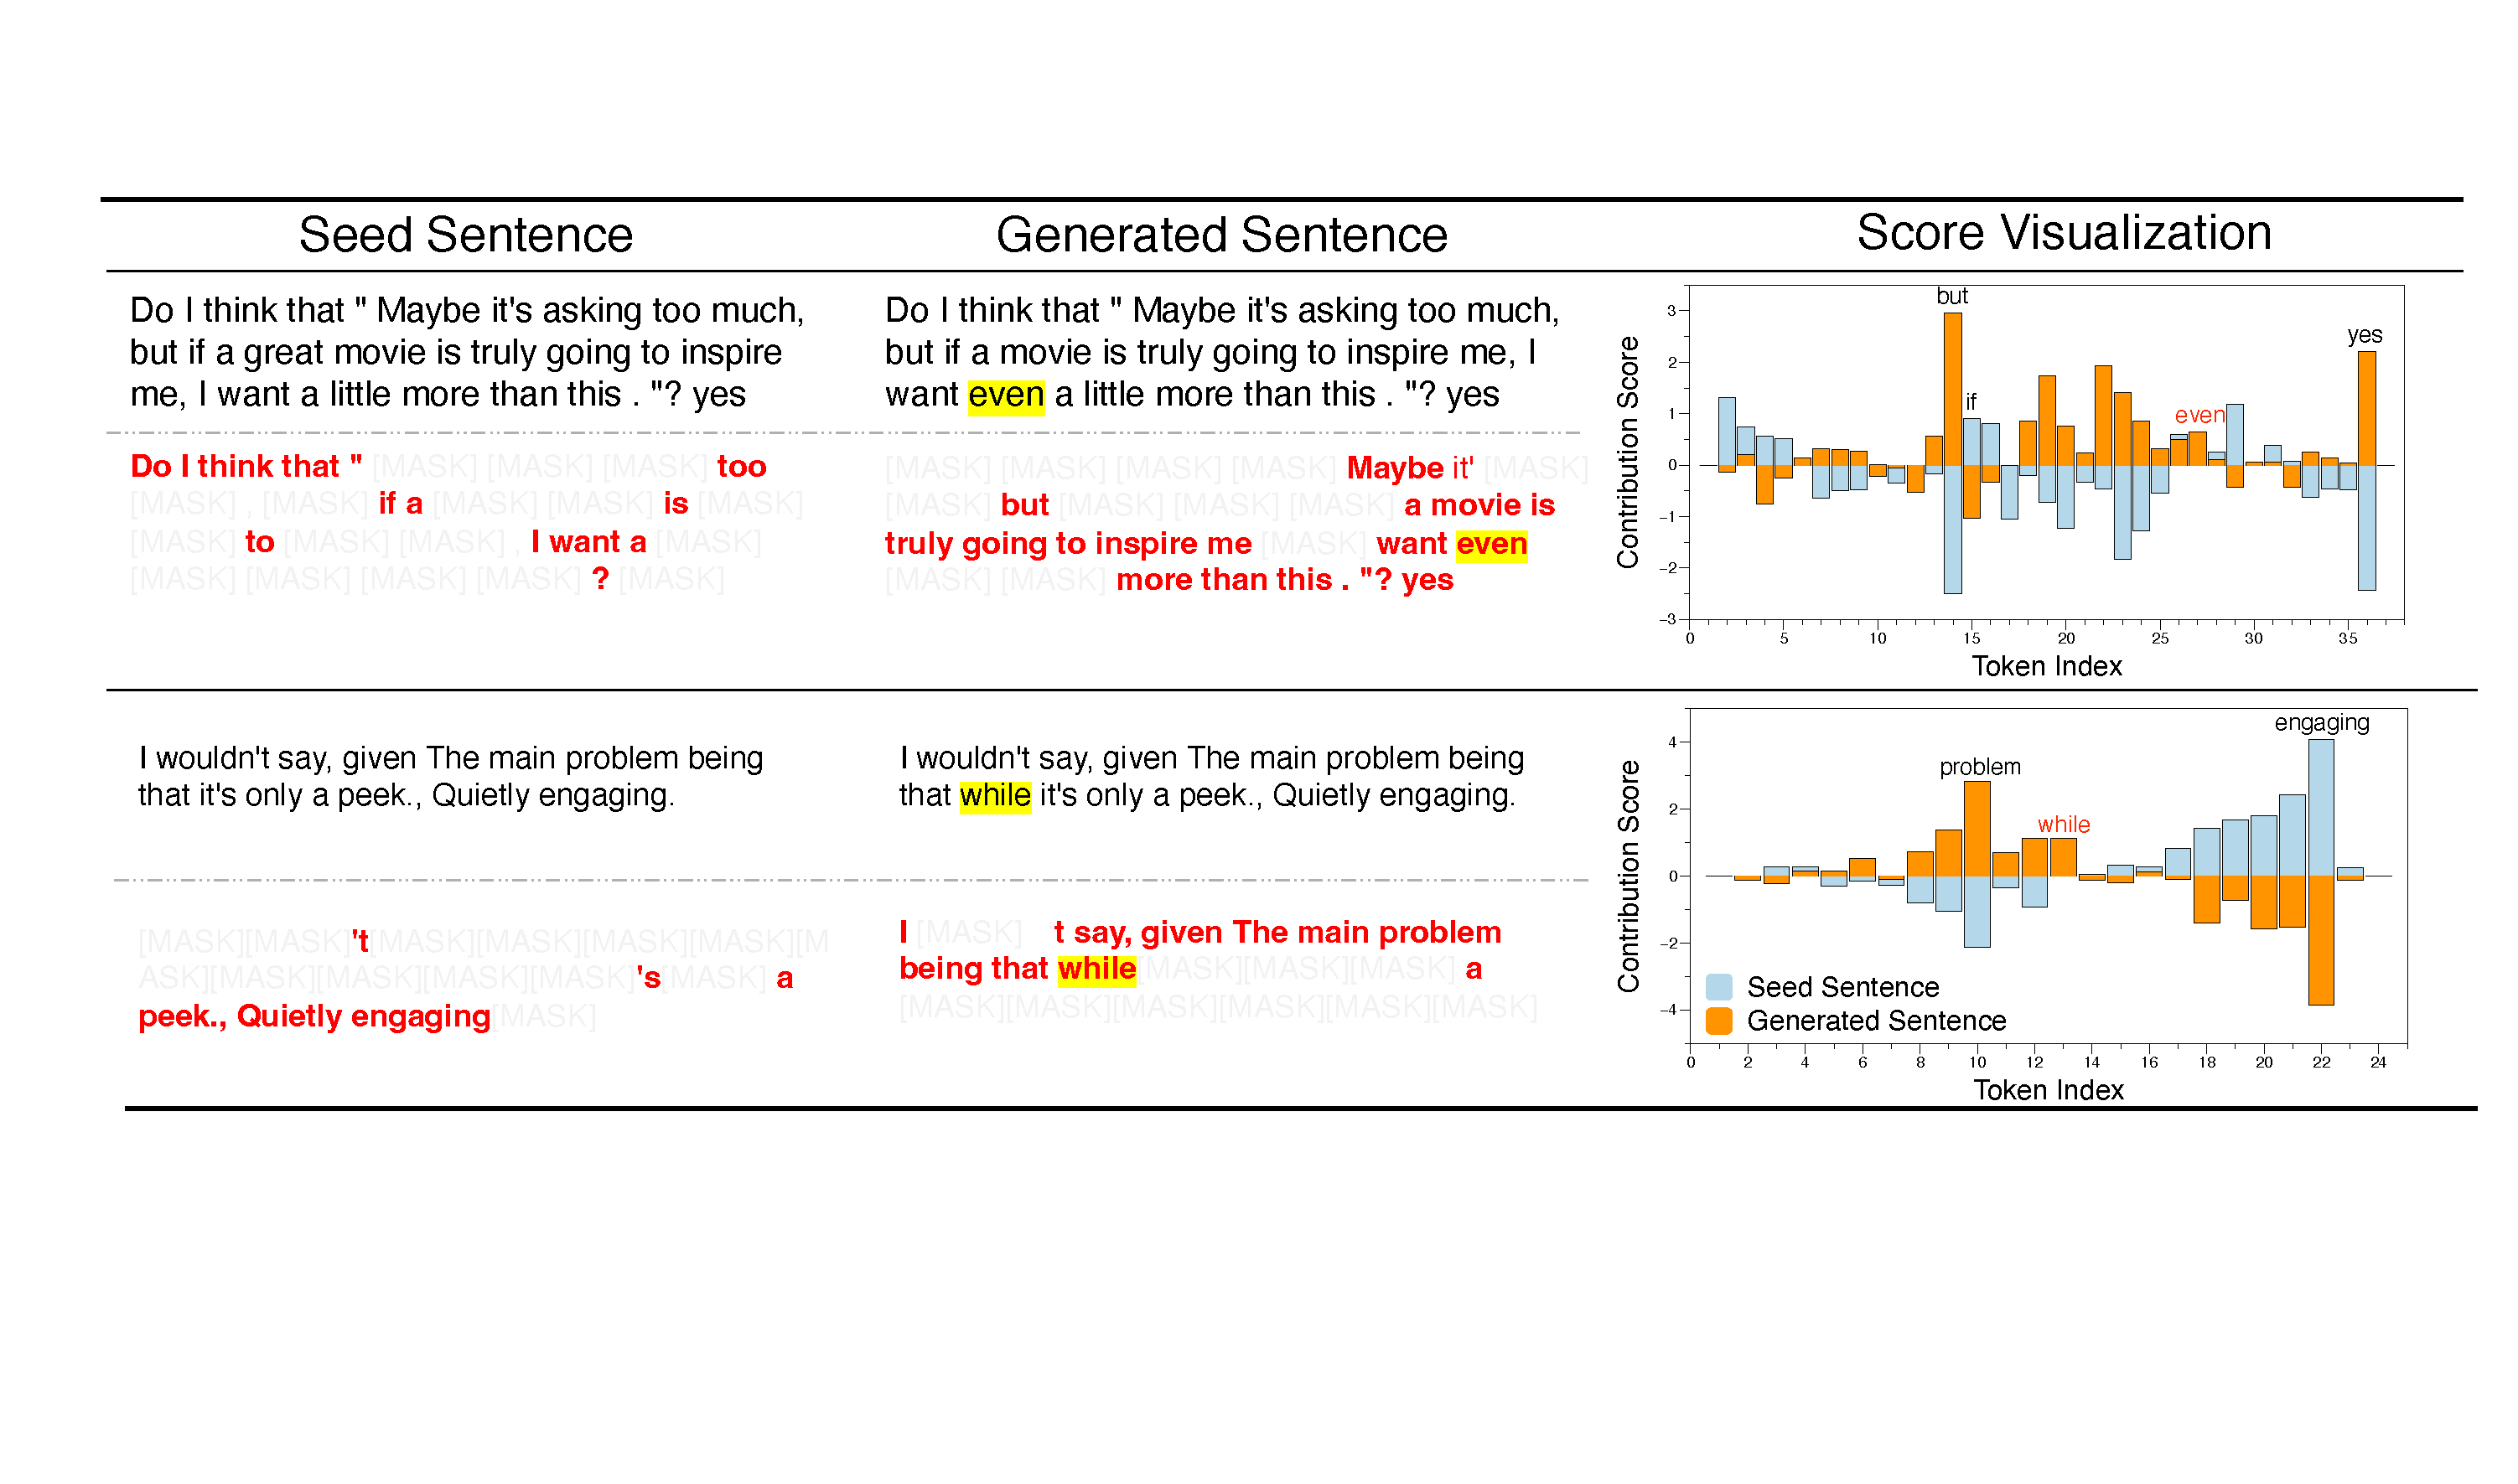
\includegraphics[width=0.8\textwidth]{figs/explain.pdf}
    \vspace{-4mm}
    \caption{Visualization of the buggy reason of two \tool generated test cases.}
    \label{fig:explain}
\end{figure*}


\MyPara{Experimental Process}
we conduct experiments to demonstrate that \tool can help developers understand the bugs in the NLP models.
Recall that \tool generates test cases by mutating seed sentences (\eg by expanding one token in the seed input). Still, it is unclear why mutating one token will cause the model to produce misclassified results.
We seek to help developers understand why such mutation will result in the misclassification. 
Existing work \cite{simin2020denas, lemna, lime} has demonstrated that the ML model prediction is dominated by a minimal set of input features (\ie tokens in input sentences). Motivated by such intuition, we identify a minimal set of input tokens that dominate the model prediction.

Formally, given a input sentence $x = [tk_1, tk_2, \cdots, tk_n]$, and the NLP model under test $f(\cdot)$, our goal is to find a masking template $T = [t_1, t_2, \cdots, t_n]$, where $t_i$ is 0 or 1, representing masking the $i^{th}$ token (\ie $tk_i$) in $x$ or not.
The template $T$ can mask some tokens in $x$ with attribute tokens, and the masked input has a high probability of retaining the original prediction $x$, denoted as
\begin{equation}
    P(f(T(x)) = f(x)) \ge P_{thresh}
    \label{eq:prob}
\end{equation}
To create such a template $T$, we first compute the contribution score of each input token using an existing explainable ML technique \cite{lemna}. We then begin with the full mask template (\ie, all tokens are masked); such full mask template definitely does not satisfy Equation \ref{eq:prob}.
We then iteratively shift one position from mask to non-mask based on the order of each token's contribution score, until the template $T$ satisfies Equation \ref{eq:prob}.
Because we iterate the size of the mask, the generated template $T$ will keep the minimum number of tokens in $x$. Moreover, since the input $x$ is an incorrect prediction, the generated template $T$ is likely to produce misclassification (i.e., the probability to be misclassified is larger than $P_{thresh}$).

\MyPara{Results} We generate a template that dominates the NLP model prediction to assist developers in understanding the false predictions. Figure \ref{fig:explain} shows the generated templates for two randomly selected seeds and their corresponding expanded test inputs.
The first example tests ``sentiments in (question, yes) form'' (LC9), and the second example tests ``negative positive with neutral content in the middle''  (LC7).
The first column shows the seed sentence, the second shows the expanded sentence, and the third shows each token's contribution score. The blue bar indicates the score for seed inputs, whereas the orange bar reflects the score for the expanded sentences.
We highlight the mutated token with yellow background and generated templates with red text. 

The results show that after mutating the seed sentence with one token, the token set that dominates the NLP model prediction has changed.
We can trace the root causes to the bias of the training data on the \lc under test; as a result, for the \lc under test, the model has a bias towards positive/negative for certain token sequence patterns. For example, LC9 has a bias toward the token sequence pattern that includes "maybe .... but ... even... yes". Thus, adding the token ``even" to the seed sentence will match one of those biased sequence patterns.
Sentences with such pattern in the training dataset are dominantly positive; thus, the models make the wrong decision on the sentence with ``even'' as positive. 
The visualization of each token's contribution score in the third column confirms our observation. Once ``even'' is added, scores of other tokens such as ``but'' and ``yes'' all change from negative to positive.
To fix the issue for LC9, we need to add more negative training samples with the format of ``maybe . .. but ... even ... yes''.
%he experimental results in Fig. \ref{fig:explain} illustrate that \tool can help developers to understand the buggy reason of the misclassification go no在,

\section{Threats to Validity}
\label{sec:threats}

Use of publicly available datasets poses an external validity threat
with respect to the generalizability of our results. We implemented
domain-spefic knowledge on publically available word sentiments
dataset~\cite{baccianella2010sentiwordnet}. We also constructed
reference CFG from publically available corpus dataset
\cite{mitchell1993treebank, nltkTreebankCorporaWebPage}. The dataset
used in our study might not be completely representative of all
English grammatical structures and English word sentiments. We
mitigate this threat by observing that they are widely used in NLP
domain~\cite{husnain2021swnvalidity} and reviewed each script and the
output logs.


\vspace{-6pt}
\section{Related Work}

\MyPara{NLP Testing}
%
With the increasing use of NLP models, evaluation of NLP models is
becoming a more important issue. Apart from the accuracy-based testing
scheme, recent works have considered model robustness as an
aspect for evaluation. Belinkov and Bisk
\textit{\etal}~\cite{belinkov2018breaknmt} aimed to fail neural machine
translation model by intentionally introducing noise in the input
text. Pinjia
\textit{\etal}~\cite{pinjia2020structinvtestingnmt,pinjia2020testnmtrt}
measured the robustness by assuming syntactic and semantic relation
between input and output of neural machine translation model.  Ribeiro
\textit{\etal}~\cite{ribeiro2018sear} proposed an approach to
generalize semantically equivalent adversarial rules. In addition,
Rychalska \textit{\etal}~\cite{rychalska2019wildnlp} measured drops in
BLEU scores by corruption operation, and compared model robustness
based on the amount of the drops. Iyyer
\textit{\etal}~\cite{iyyer2018adversarial} introduced learning-based
model for adversarial data augmentation.

In addition to the
robustness on adversarial set, various other aspects of the NLP model have been
considered for the robustness evaluation. Prabhakaran
\textit{\etal}~\cite{prabhakaran2019fairness} developed an evaluation
framework to detect unintended societal bias in NLP models. Rottger
\textit{\etal}~\cite{rottger2020hatecheck} introduced a functional
test suite for hate speech detection in the NLP model.  Ribeiro
\textit{\etal}~\cite{ribeiro2019consistencyeval} measured logical
consistency of NLP model. These techniques evaluate the robustness of
the NLP model. However, we focused on the evaluation of model capability
over multiple perspectives and produce debugging information by comparing
seed and expanded test cases.

\MyPara{Linguistic Capability Evaluation}
%
Wang \textit{\etal}~\cite{wang2018glue, wang2019superglue} proposed
multiple diagnostic datasets to evaluate NLP models. These datasets
evaluate NLP model's ability to understand input sentence via natural
language inference problems. More recently, \Cklst proposed an evaluation
method of input-output behavior defined as \lcs. \Cklst generates
behavior-guided inputs for validating the
behaviors.~\cite{marcoACL2020checklist}. Unlike prior work that relies on manual
test case generation, we used structural information in text to
generate test cases automatically.

\MyPara{NLP Model Debugging}
%
Researchers have been explaining NLP model prediction and
analyzing it for debugging the model. Ribeiro
\textit{\etal}~\cite{ribeiroSG16lime} evaluated model prediction guided by human feedback providing relevance scores for words on the model prediction. 
Interactive error analysis~\cite{wu2019errudite} also has been proposed to evaluate
model robustness. Zylberajch~\cite{zylberajch2021hildif} used influence functions to generate model explanation, and it enables interactive debugging incorporating humans feedback
explanation.
Lertvittaya~\cite{lertvittayakumjorn2020find} proposed
an approach to understand behavior of text classifier model and improve the
model by disabling irrelevant hidden features. In this work, \tool
is useful for identifying the sources of model failure as shown in RQ4.

\section{Conclusions}
\label{sec:concl}

We introduce \tool, which automatically generates test cases for testing NLP models. We evaluate the effectiveness of \tool on two popular NLP tasks.
Our study results reveal that the diversity of \tool's test cases improves model coverage and reliability. Additionally, we analyze failure-inducing cases to identify bug causes, demonstrating the correctness and utility of \tool for model evaluation.

%% Acknowledgments
%% \begin{acks}                            %% acks environment is optional
                                        %% contents suppressed with 'anonymous'
  %% Commands \grantsponsor{<sponsorID>}{<name>}{<url>} and
  %% \grantnum[<url>]{<sponsorID>}{<number>} should be used to
  %% acknowledge financial support and will be used by metadata
  %% extraction tools.
  %% This material is based upon work supported by the
  %% \grantsponsor{GS100000001}{National Science
  %%   Foundation}{http://dx.doi.org/10.13039/100000001} under Grant
  %% No.~\grantnum{GS100000001}{nnnnnnn} and Grant
  %% No.~\grantnum{GS100000001}{mmmmmmm}.  Any opinions, findings, and
  %% conclusions or recommendations expressed in this material are those
  %% of the author and do not necessarily reflect the views of the
  %% National Science Foundation.

%% We thanks Nader Al Awar, Kayvan Mansoorshahi, Jiyang Zhang, Kush Jain for their feedback on this work.

%% \end{acks}

\bibliography{bib}

%% Appendix
%\input{appendix}

%% Text of appendix \ldots

\end{document}
